% ----------------------------------------------------------------------
%
%                          Tesis.tex
%
%----------------------------------------------------------------------
%
% Este fichero contiene el "documento maestro" del documento. Lo único
% que hace es configurar el entorno LaTeX e incluir los ficheros .tex
% que contienen cada sección.
%
%----------------------------------------------------------------------
%
% Los ficheros necesarios para este documento son:
%
%       TeXiS/* : ficheros de la plantilla TeXiS.
%       Cascaras/* : ficheros con las partes del documento que no
%          son capítulos ni apéndices (portada, agradecimientos, etc.)
%       Capitulos/*.tex : capítulos de la tesis
%       Apendices/*.tex: apéndices de la tesis
%       constantes.tex: constantes LaTeX
%       config.tex : configuración de la "compilación" del documento
%       guionado.tex : palabras con guiones
%
% Para la bibliografía, además, se necesitan:
%
%       *.bib : ficheros con la información de las referencias
%
% ---------------------------------------------------------------------

\documentclass[12pt,a4paper,twoside]{book}

%
% Definimos  el   comando  \compilaCapitulo,  que   luego  se  utiliza
% (opcionalmente) en config.tex. Quedaría  mejor si también se definiera
% en  ese fichero,  pero por  el modo  en el  que funciona  eso  no es
% posible. Puedes consultar la documentación de ese fichero para tener
% más  información. Definimos también  \compilaApendice, que  tiene el
% mismo  cometido, pero  que se  utiliza para  compilar  únicamente un
% apéndice.
%
%
% Si  queremos   compilar  solo   una  parte  del   documento  podemos
% especificar mediante  \includeonly{...} qué ficheros  son los únicos
% que queremos  que se incluyan.  Esto  es útil por  ejemplo para sólo
% compilar un capítulo.
%
% El problema es que todos aquellos  ficheros que NO estén en la lista
% NO   se  incluirán...  y   eso  también   afecta  a   ficheros  de
% la plantilla...
%
% Total,  que definimos  una constante  con los  ficheros  que siempre
% vamos a querer compilar  (aquellos relacionados con configuración) y
% luego definimos \compilaCapitulo.
\newcommand{\ficherosBasicosTeXiS}{%
TeXiS/TeXiS_pream,TeXiS/TeXiS_cab,TeXiS/TeXiS_bib,TeXiS/TeXiS_cover%
}
\newcommand{\ficherosBasicosTexto}{%
constantes,guionado,Cascaras/bibliografia,config%
}
\newcommand{\compilaCapitulo}[1]{%
\includeonly{\ficherosBasicosTeXiS,\ficherosBasicosTexto,Capitulos/#1}%
}

\newcommand{\compilaApendice}[1]{%
\includeonly{\ficherosBasicosTeXiS,\ficherosBasicosTexto,Apendices/#1}%
}

%- - - - - - - - - - - - - - - - - - - - - - - - - - - - - - - - - - -
%            Preámbulo del documento. Configuraciones varias
%- - - - - - - - - - - - - - - - - - - - - - - - - - - - - - - - - - -

% Define  el  tipo  de  compilación que  estamos  haciendo.   Contiene
% definiciones  de  constantes que  cambian  el  comportamiento de  la
% compilación. Debe incluirse antes del paquete TeXiS/TeXiS.sty
%---------------------------------------------------------------------
%
%                          config.tex
%
%---------------------------------------------------------------------
%
% Contiene la  definición de constantes  que determinan el modo  en el
% que se compilará el documento.
%
%---------------------------------------------------------------------
%
% En concreto, podemos  indicar si queremos "modo release",  en el que
% no  aparecerán  los  comentarios  (creados  mediante  \com{Texto}  o
% \comp{Texto}) ni los "por  hacer" (creados mediante \todo{Texto}), y
% sí aparecerán los índices. El modo "debug" (o mejor dicho en modo no
% "release" muestra los índices  (construirlos lleva tiempo y son poco
% útiles  salvo  para   la  versión  final),  pero  sí   el  resto  de
% anotaciones.
%
% Si se compila con LaTeX (no  con pdflatex) en modo Debug, también se
% muestran en una esquina de cada página las entradas (en el índice de
% palabras) que referencian  a dicha página (consulta TeXiS_pream.tex,
% en la parte referente a show).
%
% El soporte para  el índice de palabras en  TeXiS es embrionario, por
% lo  que no  asumas que  esto funcionará  correctamente.  Consulta la
% documentación al respecto en TeXiS_pream.tex.
%
%
% También  aquí configuramos  si queremos  o  no que  se incluyan  los
% acrónimos  en el  documento final  en la  versión release.  Para eso
% define (o no) la constante \acronimosEnRelease.
%
% Utilizando \compilaCapitulo{nombre}  podemos también especificar qué
% capítulo(s) queremos que se compilen. Si no se pone nada, se compila
% el documento  completo.  Si se pone, por  ejemplo, 01Introduccion se
% compilará únicamente el fichero Capitulos/01Introduccion.tex
%
% Para compilar varios  capítulos, se separan sus nombres  con comas y
% no se ponen espacios de separación.
%
% En realidad  la macro \compilaCapitulo  está definida en  el fichero
% principal tesis.tex.
%
%---------------------------------------------------------------------


% Comentar la línea si no se compila en modo release.
% TeXiS hará el resto.
% ¡¡¡Si cambias esto, haz un make clean antes de recompilar!!!
\def\release{1}


% Descomentar la linea si se quieren incluir los
% acrónimos en modo release (en modo debug
% no se incluirán nunca).
% ¡¡¡Si cambias esto, haz un make clean antes de recompilar!!!
%\def\acronimosEnRelease{1}


% Descomentar la línea para establecer el capítulo que queremos
% compilar

% \compilaCapitulo{01Introduccion}
% \compilaCapitulo{02EstructuraYGeneracion}
% \compilaCapitulo{03Edicion}
% \compilaCapitulo{04Imagenes}
% \compilaCapitulo{05Bibliografia}
% \compilaCapitulo{06Makefile}

% \compilaApendice{01AsiSeHizo}

% Variable local para emacs, para  que encuentre el fichero maestro de
% compilación y funcionen mejor algunas teclas rápidas de AucTeX
%%%
%%% Local Variables:
%%% mode: latex
%%% TeX-master: "./Tesis.tex"
%%% End:


% Paquete de la plantilla
\usepackage{TeXiS/TeXiS}
%Incluimos el fichero con la configuración matemática
\usepackage[fleqn]{amsmath} %[fleqn] or [leqno] to put numbers of equations on the right or on left side
\usepackage{amssymb}
\usepackage{amsfonts}
\usepackage{anysize}
\usepackage{float}
\usepackage{amsthm}
\usepackage{amsmath}
%\usepackage{etoolbox}
\usepackage{verbatim}
\usepackage{mathtools}
\usepackage{enumerate}
\usepackage{geometry}
\usepackage[table]{xcolor}
\usepackage{color}
\usepackage{setspace}
\usepackage{multirow}
\usepackage{tikz}
\usetikzlibrary{babel, hobby, calc}
% \usepackage[disable]{todonotes} % notes not showed
\usepackage[colorinlistoftodos,prependcaption,textsize=normal,linecolor=cyan,backgroundcolor=lavander,bordercolor=black]{todonotes} % notes showed
% \newcommand{\note}[1]{}  %comment not showed
\newcommand{\note}[1]{\par {\bfseries \color{blue} #1 \par}} %comment showed

\definecolor{lila}{RGB}{153, 134, 244}
\definecolor{lavander}{RGB}{230, 225, 250}
\definecolor{deepblue}{rgb}{0,0,0.5}
\definecolor{deepred}{rgb}{0.6,0,0}
\definecolor{deepgreen}{rgb}{0,0.5,0}
\definecolor{Gray}{gray}{0.9}

% Margins
\geometry
{
	top=1.69in,
	bottom=1.56in,
	left=1.56in,
	right=1.04in
}

%\geometry
%{
%	top=1.3in,
%	bottom=1.2in,
%	left=1.2in,
%	right=0.8in
%}



%Theorem styles

%definition boldface title, romand body. Commonly used in definitions, conditions, problems and examples.
%plain boldface title, italicized body. Commonly used in theorems, lemmas, corollaries, propositions and conjectures.
%remark italicized title, romman body. Commonly used in remarks, notes, annotations, claims, cases, acknowledgments and conclusions.


%Para definir un nuevo estilo:

%\newtheoremstyle{stylename}% name of the style to be used
%  {spaceabove}% measure of space to leave above the theorem. E.g.: 3pt
%  {spacebelow}% measure of space to leave below the theorem. E.g.: 3pt
%  {bodyfont}% name of font to use in the body of the theorem
%  {indent}% measure of space to indent
%  {headfont}% name of head font
%  {headpunctuation}% punctuation between head and body
%  {headspace}% space after theorem head; " " = normal interword space
%  {headspec}% Manually specify head


\theoremstyle{plain}
\newtheorem{theorem}{Teorema}[section] %section restart the theorem counter at every new section.
\newtheorem{lemma}[theorem]{Lema} %it will use the same counter as the theorem environment.
\newtheorem{corollary}{Corolario}[theorem] %the counter of this new environment will be reset every time a new theorem environment is used.
\newtheorem{prop}[theorem]{Proposición}

\theoremstyle{definition}
\newtheorem{definition}[theorem]{Definición}
\newtheorem{example}[theorem]{Ejemplo}
%\AtEndEnvironment{example}{\null\hfill\qedsymbol}
\newtheorem{conj}[theorem]{Conjetura}

\theoremstyle{remark}
\newtheorem*{remark}{Nota}
\newtheorem*{obs}{Observación}

%%%%%%%%%%%%%%%%%%%%%%%%%%%%%%%%%%%%%%%%%%%%%%%%%%%%%%%%%%%%%%%%%%%%%%%%%%%
%
% To change symbol at the end of the proof
\renewcommand\qedsymbol{$\square$}
%\renewcommand\qedsymbol{$\blacksquare$}

%%%%%%%%%%%%%%%%%%%%%%%%%%%%%%%%%%%%%%%%%%%%%%%%%%%%%%%%%%%%%%%%%%%%%%%%%%%
% Syntax: [draw options] (center) (initial angle:final angle:radius)
\def\centerarc[#1](#2)(#3:#4:#5){
\draw[#1] ($(#2)+({#5*cos(#3)},{#5*sin(#3)})$) arc (#3:#4:#5); }

% Absolute value
\providecommand{\abs}[1]{\left\lvert#1\right\rvert}

% Norm
\providecommand{\norm}[1]{\left\lVert#1\right\rVert}

% Infinity norm
\providecommand{\norminf}[1]{\norm{#1}_{\infty}}

% Holomorphic
\providecommand{\holomorphic}[1]{\mathcal{H}(#1)}

% Holomorphic and bounded
\providecommand{\bholomorphic}[1]{\mathcal{H}^{\infty}(#1)}

% Fiber
%\providecommand{\fiber}[1]{\mathfrak{M}(#1)}

% Plus minus centering
\newcommand{\rpm}{\raisebox{.2ex}{$\scriptstyle\pm$}}

% Bar for the closure
\newcommand*\xbar[1]{%
   \hbox{%
     \vbox{%
       \hrule height 0.5pt % The actual bar
       \kern0.2ex%         % Distance between bar and symbol
       \hbox{%
         \kern-0.1em%      % Shortening on the left side
         \ensuremath{#1}%
         \kern-0.1em%      % Shortening on the right side
       }%
     }%
   }%
}

\newcommand{\complex}{\mathbb{C}}
\newcommand{\real}{\mathbb{R}}
\newcommand{\integer}{\mathbb{Z}}
\newcommand{\naturals}{\mathbb{N}}

\newcommand{\disk}{\mathbb{D}}
\newcommand{\closedisk}{\overline{\disk}}

\newcommand{\diam}{\operatorname{diam}}
\renewcommand{\Re}{\operatorname{Re}}
\renewcommand{\Im}{\operatorname{Im}}
\newcommand{\id}{\operatorname{id}}


%Fiber
\newcommand{\fiber}{\mathfrak{M}}

\makeatletter
\newcommand{\leqnomode}{\tagsleft@true} %to put numbers of equations on the left side
\newcommand{\reqnomode}{\tagsleft@false} %to put numbers of equations on the right side
\makeatother

% Change the appearance of the numbering of equations. Use with \usetagform{<tagform>
\newtagform{Alph}[\renewcommand{\theequation}{\Alph{equation}}]()
\newtagform{alph}[\renewcommand{\theequation}{\alph{equation}}]()
\newtagform{Roman}[\renewcommand{\theequation}{\roman{equation}}]()
\newtagform{roman}[\renewcommand{\theequation}{\roman{equation}}]()
\newtagform{scroman}[\renewcommand{\theequation}{\scshape\roman{equation}}][]

% Change line spacing of equations
%\setlength{\abovedisplayskip}{30pt}
%\setlength{\belowdisplayskip}{30pt}
%\setlength{\jot}{30pt}

% Change de alignment of equations
%\setlength{\mathindent}{1cm}

% New counter for aligns
\newcounter{align}[equation]
\renewcommand{\thealign}{\roman{align}} % style of the numbering
\newcommand{\alignno}{\refstepcounter{align}\tag{\thealign}}
\expandafter\let\expandafter\oldalignstar\csname align*\endcsname
\expandafter\def\csname align*\endcsname{\refstepcounter{equation}\oldalignstar}

% Incluimos el fichero con comandos de constantes
%---------------------------------------------------------------------
%
%                          constantes.tex
%
%---------------------------------------------------------------------
%
% Fichero que  declara nuevos comandos LaTeX  sencillos realizados por
% comodidad en la escritura de determinadas palabras
%
%---------------------------------------------------------------------

%%%%%%%%%%%%%%%%%%%%%%%%%%%%%%%%%%%%%%%%%%%%%%%%%%%%%%%%%%%%%%%%%%%%%%
% Comando:
%
%       \titulo
%
% Resultado:
%
% Escribe el título del documento.
%%%%%%%%%%%%%%%%%%%%%%%%%%%%%%%%%%%%%%%%%%%%%%%%%%%%%%%%%%%%%%%%%%%%%%
\def\titulo{Problemas geométricos que arrancan de la teoría clásica de funciones}

%%%%%%%%%%%%%%%%%%%%%%%%%%%%%%%%%%%%%%%%%%%%%%%%%%%%%%%%%%%%%%%%%%%%%%
% Comando:
%
%       \autor
%
% Resultado:
%
% Escribe el autor del documento.
%%%%%%%%%%%%%%%%%%%%%%%%%%%%%%%%%%%%%%%%%%%%%%%%%%%%%%%%%%%%%%%%%%%%%%
\def\autor{Celia de Frutos Palacios}

% Variable local para emacs, para  que encuentre el fichero maestro de
% compilación y funcionen mejor algunas teclas rápidas de AucTeX

%%%
%%% Local Variables:
%%% mode: latex
%%% TeX-master: "tesis.tex"
%%% End:


% Sacamos en el log de la compilación el copyright
\typeout{Copyright Marco Antonio and Pedro Pablo Gomez Martin}

%
% "Metadatos" para el PDF
%
\ifpdf\hypersetup{%
    pdftitle = {\titulo},
    pdfsubject = {Plantilla de Tesis},
    pdfkeywords = {Plantilla, LaTeX, tesis, trabajo de
      investigación, trabajo de Master},
    pdfauthor = {\textcopyright\ \autor},
    pdfcreator = {\LaTeX\ con el paquete \flqq hyperref\frqq},
    pdfproducer = {pdfeTeX-0.\the\pdftexversion\pdftexrevision},
    }
    \pdfinfo{/CreationDate (\today)}
\fi


%- - - - - - - - - - - - - - - - - - - - - - - - - - - - - - - - - - -
%                        Documento
%- - - - - - - - - - - - - - - - - - - - - - - - - - - - - - - - - - -
\begin{document}

\setcitestyle{authoryear,aysep={},open={(},close={)}}

% Incluimos el  fichero de definición de guionado  de algunas palabras
% que LaTeX no ha dividido como debería
%----------------------------------------------------------------
%
%                          guionado.tex
%
%----------------------------------------------------------------
%
% Fichero con algunas divisiones de palabras que LaTeX no
% hace correctamente si no se le da alguna ayuda.
%
%----------------------------------------------------------------

\hyphenation{
% a
abs-trac-to
abs-trac-tos
abs-trac-ta
abs-trac-tas
ac-tua-do-res
a-gra-de-ci-mien-tos
ana-li-za-dor
an-te-rio-res
an-te-rior-men-te
apa-rien-cia
a-pro-pia-do
a-pro-pia-dos
a-pro-pia-da
a-pro-pia-das
a-pro-ve-cha-mien-to
a-que-llo
a-que-llos
a-que-lla
a-que-llas
a-sig-na-tu-ra
a-sig-na-tu-ras
a-so-cia-da
a-so-cia-das
a-so-cia-do
a-so-cia-dos
au-to-ma-ti-za-do
% b
batch
bi-blio-gra-fía
bi-blio-grá-fi-cas
bien
bo-rra-dor
boo-l-ean-expr
% c
ca-be-ce-ra
call-me-thod-ins-truc-tion
ca-ra-théo-do-ry
cas-te-lla-no
cir-cuns-tan-cia
cir-cuns-tan-cias
co-he-ren-te
co-he-ren-tes
co-he-ren-cia
co-li-bri
co-men-ta-rio
co-mer-cia-les
co-no-ci-mien-to
cons-cien-te
con-si-de-ra-ba
con-si-de-ra-mos
con-si-de-rar-se
cons-tan-te
cons-trucción
cons-tru-ye
cons-tru-ir-se
con-tro-le
co-rrec-ta-men-te
co-rres-pon-den
co-rres-pon-dien-te
co-rres-pon-dien-tes
co-ti-dia-na
co-ti-dia-no
crean
cris-ta-li-zan
cu-rri-cu-la
cu-rri-cu-lum
cu-rri-cu-lar
cu-rri-cu-la-res
% d
de-di-ca-do
de-di-ca-dos
de-di-ca-da
de-di-ca-das
de-rro-te-ro
de-rro-te-ros
de-sa-rro-llo
de-sa-rro-llos
de-sa-rro-lla-do
de-sa-rro-lla-dos
de-sa-rro-lla-da
de-sa-rro-lla-das
de-sa-rro-lla-dor
de-sa-rro-llar
des-cri-bi-re-mos
des-crip-ción
des-crip-cio-nes
des-cri-to
des-pués
de-ta-lla-do
de-ta-lla-dos
de-ta-lla-da
de-ta-lla-das
di-a-gra-ma
di-a-gra-mas
di-se-ños
dis-po-ner
dis-po-ni-bi-li-dad
do-cu-men-ta-da
do-cu-men-to
do-cu-men-tos
% e
edi-ta-do
e-du-ca-ti-vo
e-du-ca-ti-vos
e-du-ca-ti-va
e-du-ca-ti-vas
e-la-bo-ra-do
e-la-bo-ra-dos
e-la-bo-ra-da
e-la-bo-ra-das
es-co-llo
es-co-llos
es-tu-dia-do
es-tu-dia-dos
es-tu-dia-da
es-tu-dia-das
es-tu-dian-te
e-va-lua-cio-nes
e-va-lua-do-res
exis-ten-tes
exhaus-ti-va
ex-pe-rien-cia
ex-pe-rien-cias
% f
for-ma-li-za-do
% g
ge-ne-ra-ción
ge-ne-ra-dor
ge-ne-ra-do-res
ge-ne-ran
% h
he-rra-mien-ta
he-rra-mien-tas
% i
i-dio-ma
i-dio-mas
im-pres-cin-di-ble
im-pres-cin-di-bles
in-de-xa-do
in-de-xa-dos
in-de-xa-da
in-de-xa-das
in-di-vi-dual
in-fe-ren-cia
in-fe-ren-cias
in-for-ma-ti-ca
in-gre-dien-te
in-gre-dien-tes
in-me-dia-ta-men-te
ins-ta-la-do
ins-tan-cias
% j
% k
% l
len-gua-je
li-be-ra-to-rio
li-be-ra-to-rios
li-be-ra-to-ria
li-be-ra-to-rias
li-mi-ta-do
li-te-ra-rio
li-te-ra-rios
li-te-ra-ria
li-te-ra-rias
lo-tes
% m
ma-ne-ra
ma-nual
mas-que-ra-de
ma-yor
me-mo-ria
mi-nis-te-rio
mi-nis-te-rios
mo-de-lo
mo-de-los
mo-de-la-do
mo-du-la-ri-dad
mo-vi-mien-to
% n
na-tu-ral
ni-vel
nues-tro
% o
obs-tan-te
o-rien-ta-do
o-rien-ta-dos
o-rien-ta-da
o-rien-ta-das
% p
pa-ra-le-lo
pa-ra-le-la
par-ti-cu-lar
par-ti-cu-lar-men-te
pe-da-gó-gi-ca
pe-da-gó-gi-cas
pe-da-gó-gi-co
pe-da-gó-gi-cos
pe-rio-di-ci-dad
per-so-na-je
plan-te-a-mien-to
plan-te-a-mien-tos
po-si-ción
pre-fe-ren-cia
pre-fe-ren-cias
pres-cin-di-ble
pres-cin-di-bles
pri-me-ra
pro-ble-ma
pro-ble-mas
pró-xi-mo
pu-bli-ca-cio-nes
pu-bli-ca-do
% q
% r
rá-pi-da
rá-pi-do
ra-zo-na-mien-to
ra-zo-na-mien-tos
re-a-li-zan-do
re-fe-ren-cia
re-fe-ren-cias
re-fe-ren-cia-da
re-fe-ren-cian
re-le-van-tes
re-pre-sen-ta-do
re-pre-sen-ta-dos
re-pre-sen-ta-da
re-pre-sen-ta-das
re-pre-sen-tar-lo
re-qui-si-to
re-qui-si-tos
res-pon-der
res-pon-sa-ble
% s
se-pa-ra-do
si-guien-do
si-guien-te
si-guien-tes
si-guie-ron
si-mi-lar
si-mi-la-res
si-tua-ción
% t
tem-pe-ra-ments
te-ner
trans-fe-ren-cia
trans-fe-ren-cias
% u
u-sua-rio
Unreal-Ed
% v
va-lor
va-lo-res
va-rian-te
ver-da-de-ro
ver-da-de-ros
ver-da-de-ra
ver-da-de-ras
ver-da-de-ra-men-te
ve-ri-fi-ca
% w
% x
% y
% z
}
% Variable local para emacs, para que encuentre el fichero
% maestro de compilación
%%%
%%% Local Variables:
%%% mode: latex
%%% TeX-master: "./Tesis.tex"
%%% End:


% Marcamos  el inicio  del  documento para  la  numeración de  páginas
% (usando números romanos para esta primera fase).
\frontmatter

%---------------------------------------------------------------------
%
%                          configCover.tex
%
%---------------------------------------------------------------------
%
% cover.tex
% Copyright 2009 Marco Antonio Gomez-Martin, Pedro Pablo Gomez-Martin
%
% This file belongs to the TeXiS manual, a LaTeX template for writting
% Thesis and other documents. The complete last TeXiS package can
% be obtained from http://gaia.fdi.ucm.es/projects/texis/
%
% Although the TeXiS template itself is distributed under the
% conditions of the LaTeX Project Public License
% (http://www.latex-project.org/lppl.txt), the manual content
% uses the CC-BY-SA license that stays that you are free:
%
%    - to share & to copy, distribute and transmit the work
%    - to remix and to adapt the work
%
% under the following conditions:
%
%    - Attribution: you must attribute the work in the manner
%      specified by the author or licensor (but not in any way that
%      suggests that they endorse you or your use of the work).
%    - Share Alike: if you alter, transform, or build upon this
%      work, you may distribute the resulting work only under the
%      same, similar or a compatible license.
%
% The complete license is available in
% http://creativecommons.org/licenses/by-sa/3.0/legalcode
%
%---------------------------------------------------------------------
%
% Fichero que contiene la configuración de la portada y de la
% primera hoja del documento.
%
%---------------------------------------------------------------------


% Pueden configurarse todos los elementos del contenido de la portada
% utilizando comandos.

%%%%%%%%%%%%%%%%%%%%%%%%%%%%%%%%%%%%%%%%%%%%%%%%%%%%%%%%%%%%%%%%%%%%%%
% Título del documento:
% \tituloPortada{titulo}
% Nota:
% Si no se define se utiliza el del \titulo. Este comando permite
% cambiar el título de forma que se especifiquen dónde se quieren
% los retornos de carro cuando se utilizan fuentes grandes.
%%%%%%%%%%%%%%%%%%%%%%%%%%%%%%%%%%%%%%%%%%%%%%%%%%%%%%%%%%%%%%%%%%%%%%
\tituloPortada{%
Problemas geométricos que arrancan de la teoría clásica de funciones}

%%%%%%%%%%%%%%%%%%%%%%%%%%%%%%%%%%%%%%%%%%%%%%%%%%%%%%%%%%%%%%%%%%%%%%
% Autor del documento:
% \autorPortada{Nombre}
% Se utiliza en la portada y en el valor por defecto del
% primer subtítulo de la segunda portada.
%%%%%%%%%%%%%%%%%%%%%%%%%%%%%%%%%%%%%%%%%%%%%%%%%%%%%%%%%%%%%%%%%%%%%%
\autorPortada{Celia de Frutos Palacios}

%%%%%%%%%%%%%%%%%%%%%%%%%%%%%%%%%%%%%%%%%%%%%%%%%%%%%%%%%%%%%%%%%%%%%%
% Fecha de publicación:
% \fechaPublicacion{Fecha}
% Puede ser vacío. Aparece en la última línea de ambas portadas
%%%%%%%%%%%%%%%%%%%%%%%%%%%%%%%%%%%%%%%%%%%%%%%%%%%%%%%%%%%%%%%%%%%%%%
\fechaPublicacion{Curso 2017-2018}

%%%%%%%%%%%%%%%%%%%%%%%%%%%%%%%%%%%%%%%%%%%%%%%%%%%%%%%%%%%%%%%%%%%%%%
% Imagen de la portada (y escala)
% \imagenPortada{Fichero}
% \escalaImagenPortada{Numero}
% Si no se especifica, se utiliza la imagen TODO.pdf
%%%%%%%%%%%%%%%%%%%%%%%%%%%%%%%%%%%%%%%%%%%%%%%%%%%%%%%%%%%%%%%%%%%%%%
%\imagenPortada{Imagenes/Vectorial/escudoUCM.pdf}
%\escalaImagenPortada{.3}
\imagenPortada{Imagenes/Vectorial/escudoUCM.png}
\escalaImagenPortada{.12}


%%%%%%%%%%%%%%%%%%%%%%%%%%%%%%%%%%%%%%%%%%%%%%%%%%%%%%%%%%%%%%%%%%%%%%
% Tipo de documento.
% \tipoDocumento{Tipo}
% Para el texto justo debajo del escudo.
% Si no se indica, se utiliza "TESIS DOCTORAL".
%%%%%%%%%%%%%%%%%%%%%%%%%%%%%%%%%%%%%%%%%%%%%%%%%%%%%%%%%%%%%%%%%%%%%%
\tipoDocumento{TRABAJO DE FIN DE GRADO DEL DOBLE GRADO EN INGENIERÍA INFORMÁTICA Y MATEMÁTICAS}

%%%%%%%%%%%%%%%%%%%%%%%%%%%%%%%%%%%%%%%%%%%%%%%%%%%%%%%%%%%%%%%%%%%%%%
% Institución/departamento asociado al documento.
% \institucion{Nombre}
% Puede tener varias líneas. Se utiliza en las dos portadas.
% Si no se indica aparecerá vacío.
%%%%%%%%%%%%%%%%%%%%%%%%%%%%%%%%%%%%%%%%%%%%%%%%%%%%%%%%%%%%%%%%%%%%%%
\institucion{%
Universidad Complutense de Madrid
}

%%%%%%%%%%%%%%%%%%%%%%%%%%%%%%%%%%%%%%%%%%%%%%%%%%%%%%%%%%%%%%%%%%%%%%
% Director del trabajo.
% \directorPortada{Nombre}
% Se utiliza para el valor por defecto del segundo subtítulo, donde
% se indica quién es el director del trabajo.
% Si se fuerza un subtítulo distinto, no hace falta definirlo.
%%%%%%%%%%%%%%%%%%%%%%%%%%%%%%%%%%%%%%%%%%%%%%%%%%%%%%%%%%%%%%%%%%%%%%
\directorPortada{Ángeles Prieto Yerro}

%%%%%%%%%%%%%%%%%%%%%%%%%%%%%%%%%%%%%%%%%%%%%%%%%%%%%%%%%%%%%%%%%%%%%%
% Texto del primer subtítulo de la segunda portada.
% \textoPrimerSubtituloPortada{Texto}
% Para configurar el primer "texto libre" de la segunda portada.
% Si no se especifica se indica "Memoria que presenta para optar al
% título de Doctor en Informática" seguido del \autorPortada.
%%%%%%%%%%%%%%%%%%%%%%%%%%%%%%%%%%%%%%%%%%%%%%%%%%%%%%%%%%%%%%%%%%%%%%
%\textoPrimerSubtituloPortada

%%%%%%%%%%%%%%%%%%%%%%%%%%%%%%%%%%%%%%%%%%%%%%%%%%%%%%%%%%%%%%%%%%%%%%
% Texto del segundo subtítulo de la segunda portada.
% \textoSegundoSubtituloPortada{Texto}
% Para configurar el segundo "texto libre" de la segunda portada.
% Si no se especifica se indica "Dirigida por el Doctor" seguido
% del \directorPortada.
%%%%%%%%%%%%%%%%%%%%%%%%%%%%%%%%%%%%%%%%%%%%%%%%%%%%%%%%%%%%%%%%%%%%%%

%%%%%%%%%%%%%%%%%%%%%%%%%%%%%%%%%%%%%%%%%%%%%%%%%%%%%%%%%%%%%%%%%%%%%%
% \explicacionDobleCara
% Si se utiliza, se aclara que el documento está preparado para la
% impresión a doble cara.
%%%%%%%%%%%%%%%%%%%%%%%%%%%%%%%%%%%%%%%%%%%%%%%%%%%%%%%%%%%%%%%%%%%%%%
\explicacionDobleCara

%%%%%%%%%%%%%%%%%%%%%%%%%%%%%%%%%%%%%%%%%%%%%%%%%%%%%%%%%%%%%%%%%%%%%%
% \isbn
% Si se utiliza, aparecerá el ISBN detrás de la segunda portada.
%%%%%%%%%%%%%%%%%%%%%%%%%%%%%%%%%%%%%%%%%%%%%%%%%%%%%%%%%%%%%%%%%%%%%%
%\isbn{978-84-692-7109-4}


%%%%%%%%%%%%%%%%%%%%%%%%%%%%%%%%%%%%%%%%%%%%%%%%%%%%%%%%%%%%%%%%%%%%%%
% \copyrightInfo
% Si se utiliza, aparecerá información de los derechos de copyright
% detrás de la segunda portada.
%%%%%%%%%%%%%%%%%%%%%%%%%%%%%%%%%%%%%%%%%%%%%%%%%%%%%%%%%%%%%%%%%%%%%%
\copyrightInfo{\autor}

\githubInfo{https://github.com/Celia95/TFG}
%%
%% Creamos las portadas
%%
\makeCover

% Variable local para emacs, para que encuentre el fichero
% maestro de compilación
%%%
%%% Local Variables:
%%% mode: latex
%%% TeX-master: "../Tesis.tex"
%%% End:


%---------------------------------------------------------------------
%
%                      dedicatoria.tex
%
%---------------------------------------------------------------------
%
% dedicatoria.tex
% Copyright 2009 Marco Antonio Gomez-Martin, Pedro Pablo Gomez-Martin
%
% This file belongs to the TeXiS manual, a LaTeX template for writting
% Thesis and other documents. The complete last TeXiS package can
% be obtained from http://gaia.fdi.ucm.es/projects/texis/
%
% Although the TeXiS template itself is distributed under the 
% conditions of the LaTeX Project Public License
% (http://www.latex-project.org/lppl.txt), the manual content
% uses the CC-BY-SA license that stays that you are free:
%
%    - to share & to copy, distribute and transmit the work
%    - to remix and to adapt the work
%
% under the following conditions:
%
%    - Attribution: you must attribute the work in the manner
%      specified by the author or licensor (but not in any way that
%      suggests that they endorse you or your use of the work).
%    - Share Alike: if you alter, transform, or build upon this
%      work, you may distribute the resulting work only under the
%      same, similar or a compatible license.
%
% The complete license is available in
% http://creativecommons.org/licenses/by-sa/3.0/legalcode
%
%---------------------------------------------------------------------
%
% Contiene la página de dedicatorias.
%
%---------------------------------------------------------------------

\dedicatoriaUno{%
\emph{
A mis padres\\
y\hspace*{10ex} \\
a tí, lector carísimo%
}%
}

%\dedicatoriaDos{%
%\emph{%
%I can't go to a restaurant and\\%
%order food because I keep looking\\%
%at the fonts on the menu.\\%
%Donald Knuth%
%}%
%}

\makeDedicatorias

% Variable local para emacs, para que encuentre el fichero
% maestro de compilación
%%%
%%% Local Variables:
%%% mode: latex
%%% TeX-master: "../Tesis.tex"
%%% End:


%%---------------------------------------------------------------------
%
%                      agradecimientos.tex
%
%---------------------------------------------------------------------
%
% agradecimientos.tex
% Copyright 2009 Marco Antonio Gomez-Martin, Pedro Pablo Gomez-Martin
%
% This file belongs to the TeXiS manual, a LaTeX template for writting
% Thesis and other documents. The complete last TeXiS package can
% be obtained from http://gaia.fdi.ucm.es/projects/texis/
%
% Although the TeXiS template itself is distributed under the 
% conditions of the LaTeX Project Public License
% (http://www.latex-project.org/lppl.txt), the manual content
% uses the CC-BY-SA license that stays that you are free:
%
%    - to share & to copy, distribute and transmit the work
%    - to remix and to adapt the work
%
% under the following conditions:
%
%    - Attribution: you must attribute the work in the manner
%      specified by the author or licensor (but not in any way that
%      suggests that they endorse you or your use of the work).
%    - Share Alike: if you alter, transform, or build upon this
%      work, you may distribute the resulting work only under the
%      same, similar or a compatible license.
%
% The complete license is available in
% http://creativecommons.org/licenses/by-sa/3.0/legalcode
%
%---------------------------------------------------------------------
%
% Contiene la página de agradecimientos.
%
% Se crea como un capítulo sin numeración.
%
%---------------------------------------------------------------------

\chapter{Agradecimientos}

\cabeceraEspecial{Agradecimientos}

\begin{FraseCelebre}
\begin{Frase}
A todos los que la presente vieren y entendieren.
\end{Frase}
\begin{Fuente}
Inicio de las Leyes Orgánicas. Juan Carlos I
\end{Fuente}
\end{FraseCelebre}

Groucho Marx decía que encontraba a la televisión muy educativa porque
cada vez que alguien la encendía, él se iba a otra habitación a leer
un libro. Utilizando un esquema similar, nosotros queremos agradecer
al Word de Microsoft el habernos forzado a utilizar \LaTeX. Cualquiera
que haya intentado escribir un documento de más de 150 páginas con
esta aplicación entenderá a qué nos referimos. Y lo decimos porque
nuestra andadura con \LaTeX\ comenzó, precisamente, después de
escribir un documento de algo más de 200 páginas. Una vez terminado
decidimos que nunca más pasaríamos por ahí. Y entonces caímos en
\LaTeX.

Es muy posible que hubíeramos llegado al mismo sitio de todas formas,
ya que en el mundo académico a la hora de escribir artículos y
contribuciones a congresos lo más extendido es \LaTeX. Sin embargo,
también es cierto que cuando intentas escribir un documento grande
en \LaTeX\ por tu cuenta y riesgo sin un enlace del tipo ``\emph{Author
  instructions}'', se hace cuesta arriba, pues uno no sabe por donde
empezar.

Y ahí es donde debemos agradecer tanto a Pablo Gervás como a Miguel
Palomino su ayuda. El primero nos ofreció el código fuente de una
programación docente que había hecho unos años atrás y que nos sirvió
de inspiración (por ejemplo, el fichero \texttt{guionado.tex} de
\texis\ tiene una estructura casi exacta a la suya e incluso puede
que el nombre sea el mismo). El segundo nos dejó husmear en el código
fuente de su propia tesis donde, además de otras cosas más
interesantes pero menos curiosas, descubrimos que aún hay gente que
escribe los acentos españoles con el \verb+\'{\i}+.

No podemos tampoco olvidar a los numerosos autores de los libros y
tutoriales de \LaTeX\ que no sólo permiten descargar esos manuales sin
coste adicional, sino que también dejan disponible el código fuente.
Estamos pensando en Tobias Oetiker, Hubert Partl, Irene Hyna y
Elisabeth Schlegl, autores del famoso ``The Not So Short Introduction
to \LaTeXe'' y en Tomás Bautista, autor de la traducción al español. De
ellos es, entre otras muchas cosas, el entorno \texttt{example}
utilizado en algunos momentos en este manual.

También estamos en deuda con Joaquín Ataz López, autor del libro
``Creación de ficheros \LaTeX\ con {GNU} Emacs''. Gracias a él dejamos
de lado a WinEdt y a Kile, los editores que por entonces utilizábamos
en entornos Windows y Linux respectivamente, y nos pasamos a emacs. El
tiempo de escritura que nos ahorramos por no mover las manos del
teclado para desplazar el cursor o por no tener que escribir
\verb+\emph+ una y otra vez se lo debemos a él; nuestro ocio y vida
social se lo agradecen.

Por último, gracias a toda esa gente creadora de manuales, tutoriales,
documentación de paquetes o respuestas en foros que hemos utilizado y
seguiremos utilizando en nuestro quehacer como usuarios de
\LaTeX. Sabéis un montón.

Y para terminar, a Donal Knuth, Leslie Lamport y todos los que hacen y
han hecho posible que hoy puedas estar leyendo estas líneas.

\endinput
% Variable local para emacs, para  que encuentre el fichero maestro de
% compilación y funcionen mejor algunas teclas rápidas de AucTeX
%%%
%%% Local Variables:
%%% mode: latex
%%% TeX-master: "../Tesis.tex"
%%% End:


%---------------------------------------------------------------------
%
%                      resumen.tex
%
%---------------------------------------------------------------------
%
% Contiene el capítulo del resumen.
%
% Se crea como un capítulo sin numeración.
%
%---------------------------------------------------------------------

\chapter{Resumen}
\cabeceraEspecial{Resumen}

\begin{FraseCelebre}
\begin{Frase}
Frase célebre pedante
\end{Frase}
\begin{Fuente}
Fuente de la frase célebre pedante
\end{Fuente}
\end{FraseCelebre}

Resumen de lo que hago en mi TFG

\endinput
% Variable local para emacs, para  que encuentre el fichero maestro de
% compilación y funcionen mejor algunas teclas rápidas de AucTeX
%%%
%%% Local Variables:
%%% mode: latex
%%% TeX-master: "../Tesis.tex"
%%% End:


%---------------------------------------------------------------------
%
%                      abstract.tex
%
%---------------------------------------------------------------------
%
% Contiene el capítulo del abstract.
%
% Se crea como un capítulo sin numeración.
%
%---------------------------------------------------------------------

\chapter{Abstract}
\cabeceraEspecial{Abstract}

This paper aims to show the behaviour of some functions of a complex variable on the boundary of the open unit disk, especially the holomorphic and harmonic functions (on the open disk). With this objective, theoretical results and their proofs are detailed and examples of different nature are provided. Currently we have computer tools which allow us to enrich the usual analytical study carried out. Therefore, part of this work consist of designing appropriate applications which allow us to visualize, analyse and illustrate some of these classic problems such as the well-known Dirichlet problem, solved by the Poisson integral. \\

\textbf{Keywords}: Poisson integral, Fatou theorem, Carathéodory theorem, Blaschke product, Banach algebra, spectrum, cluster set, angular derivative, Schwarz-Pick lemma, Julia theorem. \\


\endinput
% Variable local para emacs, para  que encuentre el fichero maestro de
% compilación y funcionen mejor algunas teclas rápidas de AucTeX
%%%
%%% Local Variables:
%%% mode: latex
%%% TeX-master: "../Tesis.tex"
%%% End:


%%---------------------------------------------------------------------
%
%                      palabras_clave.tex
%
%---------------------------------------------------------------------
%
% Contiene el capítulo con las palabras clave.
%
% Se crea como un capítulo sin numeración.
%
%---------------------------------------------------------------------

\chapter{Palabras clave}
\cabeceraEspecial{Palabras clave}

\begin{itemize}
    \item No más de 10 palabras clave
\end{itemize}

\endinput
% Variable local para emacs, para  que encuentre el fichero maestro de
% compilación y funcionen mejor algunas teclas rápidas de AucTeX
%%%
%%% Local Variables:
%%% mode: latex
%%% TeX-master: "../Tesis.tex"
%%% End:


%%---------------------------------------------------------------------
%
%                      keywords.tex
%
%---------------------------------------------------------------------
%
% Contiene el capítulo con las palabras clave.
%
% Se crea como un capítulo sin numeración.
%
%---------------------------------------------------------------------

\chapter{Keywords}
\cabeceraEspecial{Keywords}

\begin{itemize}
    \item No more than 10 keywords
\end{itemize}

\endinput
% Variable local para emacs, para  que encuentre el fichero maestro de
% compilación y funcionen mejor algunas teclas rápidas de AucTeX
%%%
%%% Local Variables:
%%% mode: latex
%%% TeX-master: "../Tesis.tex"
%%% End:\endinput



\ifx\generatoc\undefined
\else
%---------------------------------------------------------------------
%
%                          TeXiS_toc.tex
%
%---------------------------------------------------------------------
%
% TeXiS_toc.tex
% Copyright 2009 Marco Antonio Gomez-Martin, Pedro Pablo Gomez-Martin
%
% This file belongs to TeXiS, a LaTeX template for writting
% Thesis and other documents. The complete last TeXiS package can
% be obtained from http://gaia.fdi.ucm.es/projects/texis/
%
% This work may be distributed and/or modified under the
% conditions of the LaTeX Project Public License, either version 1.3
% of this license or (at your option) any later version.
% The latest version of this license is in
%   http://www.latex-project.org/lppl.txt
% and version 1.3 or later is part of all distributions of LaTeX
% version 2005/12/01 or later.
%
% This work has the LPPL maintenance status `maintained'.
%
% The Current Maintainers of this work are Marco Antonio Gomez-Martin
% and Pedro Pablo Gomez-Martin
%
%---------------------------------------------------------------------
%
% Contiene  los  comandos  para  generar los  índices  del  documento,
% entendiendo por índices las tablas de contenidos.
%
% Genera  el  índice normal  ("tabla  de  contenidos"),  el índice  de
% figuras y el de tablas. También  crea "marcadores" en el caso de que
% se esté compilando con pdflatex para que aparezcan en el PDF.
%
%---------------------------------------------------------------------


% Primero un poquito de configuración...


% Pedimos que inserte todos los epígrafes hasta el nivel \subsection en
% la tabla de contenidos.
\setcounter{tocdepth}{2}

% Le  pedimos  que nos  numere  todos  los  epígrafes hasta  el  nivel
% \subsubsection en el cuerpo del documento.
\setcounter{secnumdepth}{3}


% Creamos los diferentes índices.

% Lo primero un  poco de trabajo en los marcadores  del PDF. No quiero
% que  salga una  entrada  por cada  índice  a nivel  0...  si no  que
% aparezca un marcador "Índices", que  tenga dentro los otros tipos de
% índices.  Total, que creamos el marcador "Índices".
% Antes de  la creación  de los índices,  se añaden los  marcadores de
% nivel 1.

\ifpdf
   \pdfbookmark{Índices}{indices}
\fi

% Tabla de contenidos.
%
% La  inclusión  de '\tableofcontents'  significa  que  en la  primera
% pasada  de  LaTeX  se  crea   un  fichero  con  extensión  .toc  con
% información sobre la tabla de contenidos (es conceptualmente similar
% al  .bbl de  BibTeX, creo).  En la  segunda ejecución  de  LaTeX ese
% documento se utiliza para  generar la verdadera página de contenidos
% usando la  información sobre los  capítulos y demás guardadas  en el
% .toc
\ifpdf
   \pdfbookmark[1]{Tabla de contenidos}{tabla de contenidos}
\fi

\cabeceraEspecial{\'Indice}

\tableofcontents

\newpage

% Índice de figuras
%
% La idea es semejante que para  el .toc del índice, pero ahora se usa
% extensión .lof (List Of Figures) con la información de las figuras.

%\cabeceraEspecial{\'Indice de figuras}

%\ifpdf
%   \pdfbookmark[1]{Índice de figuras}{indice de figuras}
%\fi

%\listoffigures

%\newpage

% Índice de tablas
% Como antes, pero ahora .lot (List Of Tables)

%\ifpdf
%   \pdfbookmark[1]{Índice de tablas}{indice de tablas}
%\fi

%\cabeceraEspecial{\'Indice de tablas}

%\listoftables

%\newpage

% Variable local para emacs, para  que encuentre el fichero maestro de
% compilación y funcionen mejor algunas teclas rápidas de AucTeX

%%%
%%% Local Variables:
%%% mode: latex
%%% TeX-master: "../Tesis.tex"
%%% End:

\fi

% Marcamos el  comienzo de  los capítulos (para  la numeración  de las
% páginas) y ponemos la cabecera normal
\mainmatter
\restauraCabecera

%---------------------------------------------------------------------
%
%                          Capítulo 1
%
%---------------------------------------------------------------------

%\chapter{Introducción}

%\begin{FraseCelebre}
%\begin{Frase}
%...
%\end{Frase}
%\begin{Fuente}
%...
%\end{Fuente}
%\end{FraseCelebre}

%\begin{resumen}
%...
%\end{resumen}

%-------------------------------------------------------------------
\chapter*{Introducción}
\addcontentsline{toc}{chapter}{Introducción}
\label{cap1:sec:introduccion}

Introducción del TFG
...

% Variable local para emacs, para  que encuentre el fichero maestro de
% compilación y funcionen mejor algunas teclas rápidas de AucTeX
%%%
%%% Local Variables:
%%% mode: latex
%%% TeX-master: "../Tesis.tex"
%%% End:

\chapter{Teorema de Fatou y Teorema de Carathéodory}

\begin{comment}
    \begin{theorem}[Lema de Schwart]
        Sea $f: \disk \rightarrow \closedisk$ una función $\in \holomorphic{\disk}$ tal que $f(0) = 0$. Entonces:
        \begin{itemize}
            \item $\abs{f(z)} \leq \abs{z}$ para todo $z \in \disk$.
            \item Si para algún $z_0 \not = 0$ tenemos que $\abs{f(z_0)} = \abs{z_0}$, entonces existe $\alpha \in \complex, \abs{\alpha} = 1$ tal que $f(z)=\alpha z$.
        \end{itemize}
    \end{theorem}

    \begin{proof}
        Sea $f(z) = a_1z + \cdots$ la serie de potencias de $f$. El término constante es $0$ puesto que suponemos que $f(0) = 0$. Entonces $f(z)/z$ es una función holomorfa y
        \begin{equation*}
            \abs{\dfrac{f(z)}{z}} < 1/r \text{ para } \abs{z} = r < 1
        \end{equation*}
    \end{proof}
\end{comment}

\section{Integral de Poisson y Teorema de Fatou}

\subsection{La Integral de Poisson}

\begin{definition}
    Se llama núcleo de Poisson a la función $P$ definida por
    \begin{equation}
        \label{poisson1}
        P:(r,t) \in [0,1)\times \real \mapsto P_r(t) = \sum_{n=-\infty}^{\infty} r^{\abs{n}}e^{int}.
    \end{equation}

    Podemos considerar el núcleo de Poisson como una función de dos variables $r$ y $t$ o como una familia de funciones de $t$ que dependen de $r$.

    Dados $z=re^{i \theta}$, con $r \in [0,1)$ y $\theta \in \real$ se tiene que
    \begin{equation}
        \label{poisson2}
        P_r(\theta - t) = \Re \left[ \dfrac{e^{it} + z}{e^{it} - z} \right] = \dfrac{1 - r^2}{1 - 2r \cos (\theta - t) + r^2}
    \end{equation}
    para todo $t \in \real$. En efecto:

    \begin{multline*}
        P_r(t) = \sum_{n=-\infty}^{\infty} r^{\abs{n}}e^{int} = 1 + \sum_{n=1}^{\infty} r^n e^{int} + \sum_{n=1}^{\infty} r^n e^{-int} = 1 + \sum_{n=1}^{\infty} r^n (e^{int} + e^{-int}) = \\
        1 + \sum_{n=1}^{\infty} r^n 2 \Re(e^{int}) = \Re \left[ 1 + 2 \sum_{n=1}^{\infty} (r e^{it})^n  \right] = \Re \left[ 1 + 2 \dfrac{re^{it}}{1-re^{it}} \right] = \Re \left[\dfrac{1 + re^{it}}{1-re^{it}} \right].
    \end{multline*}
    \\ \par
    Por otra parte
    \begin{equation*}
        \Re \left[ \dfrac{1 + re^{it}}{1-re^{it}} \right] = \Re \left[ \dfrac{(1 + re^{it})(1 - re^{it})}{\abs{1-re^{it}}^2} \right] = \dfrac{1 - r^2}{1 - 2r \cos t + r^2}.
    \end{equation*}
\end{definition}

\newpage

\textbf{Propiedades del núcleo de Poisson:}% \\ \par

%De \ref{poisson1} tenemos que
\begin{equation}
    \dfrac{1}{2 \pi} \int_{- \pi}^{\pi} P_r (t) dt = 1, \forall r \in [0,1).
\end{equation}

%De \ref{poisson2} se sigue que
\begin{equation}
    P_r(t) > 0, \forall r \in [0,1), t \in \real
\end{equation}

\begin{equation}
    P_r(t) = P_r(-t), \forall r \in [0,1), t \in \real
\end{equation}

\begin{equation}
    P_r(t) < P_r(\delta), 0 < \delta < \abs{t} \leq \pi
\end{equation}

\begin{equation}
    \lim_{r \rightarrow 1} P_r(\delta) = 0, \forall \delta \in (0,\pi]
\end{equation}

\bigskip \par

\begin{definition}
    Se llama integral de Poisson de una función $f \in L^1(e^{it})$ a la función $F$ dada por
    \begin{equation*}
        F: z=re^{i \theta} \in \disk \mapsto F(re^{i \theta}) = \dfrac{1}{2 \pi} \int_{- \pi}^{\pi} P_r (\theta - t) f(e^{it}) dt.
    \end{equation*}

    Algunas veces nos convendrá referirnos a ella como $F=P[f]$.
\end{definition}

\bigskip

Además si $f$ lleva $\partial \disk$ en los reales, \ref{poisson2} nos muestra que

\begin{equation*}
     P[f] = \Re \left[ \dfrac{1}{2} \int_{-\pi}^{\pi} \dfrac{e^{it} + z}{e^{it} - z} f(t) dt \right].
\end{equation*}

\subsection{Teorema de Fatou}

Para demostrar el Teorema de Fatou nos vamos a basar en unos resultados clásicos del libro \citet[chap. 11]{rudin}.

\begin{theorem}
    \label{fatouaux1}
    Si $f \in L^1(\partial \disk)$ y $F = P[f]$, entonces
    \begin{equation*}
        \lim_{r \rightarrow 1} F(re^{i \theta}) = f(e^{i \theta})
    \end{equation*}
\end{theorem}

\begin{theorem}
    \label{fatouaux2}
    Sean $f \in C (\partial \disk), F=P[f]$ y
    \begin{equation*}
        u(re^{i \theta}) =
        \begin{cases}
            f(re^{i\theta}) & \text{si } r=1\\ F(re^{i\theta}) & \text{si } 0 \leq r<1
        \end{cases}
    \end{equation*}
    Entonces $u$ es una función continua en el disco cerrado $\closedisk$ que es armónica en $\disk$ .
\end{theorem}

\begin{theorem}[Teorema de Fatou]
    Para toda función $f \in \bholomorphic{\disk}$, existe una función $f^* \in L^{\infty} (\partial \disk)$ definida por
    \begin{equation}
        \label{fatou1}
        f^*(e^{it}) = \lim_{r \rightarrow 1} f(re^{it})
    \end{equation}
    en casi todo punto.

    Se tiene la igualdad $\norminf{f} = \norminf{f^*}$. Para todo $z \in U$, la fórmula integral de Cauchy
    \begin{equation}
        \label{fatou2}
        f(z) = \dfrac{1}{2 \pi i} \int_{\gamma} \dfrac{f^*(\xi)}{\xi - z} d\xi
    \end{equation}

    se satisface, donde $\gamma$ es el círculo unidad positivamente orientado: $\gamma(t) = e^{it}, 0 \leq t \leq 2 \pi$.

    Las funciones $f^* \in L^{\infty}(\partial \disk)$ que se obtienen mediante este procedimiento son precisamente aquellas que cumplen la siguiente relación

    \begin{equation}
        \label{fatou3}
        \dfrac{1}{2 \pi i} \int_{-\pi}^{\pi} f^*(e^{it})e^{-int} dt = 0, n = -1,-2, \dots
    \end{equation}
\end{theorem}

\begin{proof}
    La existencia de $f^*$ se sigue de los teoremas \ref{fatouaux1} y \ref{fatouaux2}.

    Por \ref{fatou1}, tenemos que $\norminf{f^*} \leq \norminf{f}$.

    Si $z \in U$ y $\abs{z} < r < 1$, tomemos $\gamma_r(t) = r e^{it}, 0 \leq t \leq 2\pi$. Entonces,
    \begin{equation*}
        f(z) = \dfrac{1}{2 \pi i} \int_{\gamma_r} \dfrac{f(\xi)}{\xi - z} d\xi =
        \dfrac{r}{2 \pi} \int_{-\pi}^{\pi} \dfrac{f(re^{it})}{re^{it} - z}e^{it} dt
    \end{equation*}

    Sea $\{r_n\}$ una sucesión tal que $r_n \rightarrow 1$. Por el teorema de la convergencia dominada de Lebesgue tenemos %quizá puedes aclarar a qué sucesión de funciones f_n lo aplicas, para que se vea mejor y no haga falta más abajo repetir el argumento.
    \begin{equation}
        \label{fatou_proof}
        f(z) = \dfrac{1}{2 \pi} \int_{-\pi}^{\pi} \dfrac{f^* (e^{it})}{1 - ze^{-it}} dt
    \end{equation}
    Por lo que ya hemos probado \ref{fatou2}. Por el teorema de Cauchy, se sigue que
    \begin{equation*}
        \int_{\gamma_r} f(\xi)\xi^n d\xi = 0, n = 0, 1, \dots
    \end{equation*}

    Tomando de nuevo una sucesión $\{r_n\}$ que tienda a 1, el teorema de la convergencia dominada garantiza que $f^*$ cumple \ref{fatou3}. Además, podemos convertir \ref{fatou_proof} en una integral de Poisson, si $z = re^{i \theta}$,
    \begin{equation*}
         \begin{split}
             f(z) &  = \dfrac{1}{2 \pi} \int_{- \pi}^{\pi} f^*(e^{it}) \sum_{n=0}^{\infty} r^n e^{in(\theta - t)} dt =  \dfrac{1}{2 \pi} \int_{- \pi}^{\pi} f^*(e^{it}) \sum_{n=-\infty}^{\infty} r^{\abs{n}} e^{in(\theta - t)} dt = \\
                  & =  \dfrac{1}{2 \pi} \int_{- \pi}^{\pi} P_r(\theta - t) f^*(e^{it}) dt
         \end{split}
    \end{equation*}

    De esto concluimos que $\norminf{f} \leq \norminf{f^*}$, así que ambas normas coinciden.
\end{proof}

\section{Teorema de Carathéodory}

\begin{definition}{Aplicación conforme}
    Sean $U$ y $V \subset \complex^n$. Una aplicación $f: U \rightarrow V$ se llama conforme en un punto $u \in U$ si preserva la orientación y los ángulos entre curvas que pasan por $u$.
\end{definition}

\begin{prop}
    Sea $U \subset \complex$. Una aplicación $f: U \rightarrow \complex$ es conforme en $U$ si y solo si $f \in \holomorphic{U}$ y $f'(z) \not = 0 \, \forall z \in U$.
    %a f tienes que pedirle que admita derivadas parciales con respecto a x e y y sean continuas. En la implicación => derivas con respecto a ambas.
\end{prop}

\begin{proof}
    $(\Leftarrow)$ Supongamos que $f(z)$ es una función holomorfa en $U$ tal que $f'(z) \not = 0$ para $z \in U$ y consideremos $f:z \rightarrow w=f(z)$. Sea $\gamma: [a,b] \rightarrow U$ una curva suave. Consideremos $\lambda = (f \circ  \gamma)(t)$. Por la regla de la cadena, $\lambda$ es continuamente diferenciable y como $f'(\gamma(t)) \not = 0$, tenemos
    \begin{equation}
        \label{cadena}
        \lambda'(t) = f'(\gamma(t))\gamma'(t).
    \end{equation}
    Por lo tanto, $\lambda$ es una curva suave en el plano $w$.

    Sean $\gamma_1, \gamma_2: [a,b] \rightarrow U$ curvas suaves tales que $c=\gamma_1(a) = \gamma_2(a)$. Definimos el ángulo $\theta$ entre $\gamma_1$ y $\gamma_2$ en $c$ como el argumento de $\frac{\gamma_2'(a)}{\gamma_1'(a)}$. Como el argumento es aditivo para la multiplicación de funciones, tenemos que
    \begin{equation*}
    \begin{split}
        \arg \lambda_1'(a) = \arg f'(c) + \arg \gamma_1'(a)\\
        \arg \lambda_2'(a) = \arg f'(c) + \arg \gamma_2'(a)
    \end{split}
    \end{equation*}

    y entonces
    \begin{equation*}
        \arg  \frac{\lambda_2'(a)}{\lambda_1'(a)} = \arg \lambda_2'(a) - \arg \lambda_1'(a) = \arg \gamma_2'(a) - \arg \gamma_1'(a) = \arg  \frac{\gamma_2'(a)}{\gamma_1'(a)}.
    \end{equation*}

    Así, el ángulo entre las curvas $\lambda_1$ y $\lambda_2$ en $d = \lambda_1(a) = \lambda_2(a)$ es igual al ángulo $\theta$ entre las curvas $\gamma_1$ y $\gamma_2$ en $c$. \\ \par

    \begin{comment}    
    $(\Leftarrow)$ Supongamos que $f(z)$ es una función holomorfa en $U$ tal que $f'(z) \not = 0$ para $z \in U$ y consideremos $f:z \rightarrow w=f(z)$. Sea $\gamma: [a,b] \rightarrow U$ una curva suave. Consideremos $\lambda = (f \circ  \gamma)(t)$. Por la regla de la cadena, $\lambda$ es continuamente diferenciable y como $f'(\gamma(t)) \not = 0$, tenemos
    \begin{equation}
        \label{cadena}
        \lambda'(t) = f'(\gamma(t))\gamma'(t).
    \end{equation}

    Por lo tanto, $\lambda$ es una curva suave en el plano $w$.

    Sean $\gamma_1, \gamma_2: [a,b] \rightarrow U$ curvas suaves tales que $c=\gamma_1(a) = \gamma_2(a)$. Definimos el ángulo $\theta$ entre $\gamma_1$ y $\gamma_2$ en $c$ como el argumento de $\frac{\gamma_2'(a)}{\gamma_1'(a)}$, es decir,
    \begin{equation*}
        \dfrac{\gamma_2'(a)}{\gamma_1'(a)} = \abs{\dfrac{\gamma_2'(a)}{\gamma_1'(a)}} e^{i\theta}.
    \end{equation*}

    La aplicación $f$ lleva las curvas $\gamma_1$ y $\gamma_2$ en curvas suaves $\lambda_1=f(\gamma_1)$ y $\lambda_2=f(\gamma_2)$ que tienen como punto inicial $d=f(c)$. Por \ref{cadena} tenemos
    \begin{equation*}
        \dfrac{\lambda_2'(a)}{\lambda_1'(a)} = \dfrac{\gamma_2'(a)}{\gamma_1'(a)}
    \end{equation*}
    entonces el ángulo entre las curvas $\lambda_1$ y $\lambda_2$ en $d = \lambda_1(a) = \lambda_2(a)$ es igual al ángulo $\theta$ entre las curvas $\gamma_1$ y $\gamma_2$ en $c$. \\ \par
    \end{comment}

    $(\Rightarrow)$ Supongamos que $f$ es conforme. Fijamos $z$ un punto arbitrario de $U$, y elegimos $\varepsilon > 0$ tal que $D(z, \varepsilon) \subset U$. Consideremos la familia de curvas suaves $\gamma_{\theta}(t) = z + te^{i \theta}, 0 \leq t \leq \varepsilon, \theta \in \real$. Nótese que el ángulo entre $\gamma_0$ y $\gamma_{\theta}$ en $z$ es $\theta$.


    Tomemos $\lambda_\theta = (f \circ  \gamma_\theta)(t)$ una familia de curvas. Como $f$ es conforme, el ángulo entre $\lambda_0$ y $\lambda_{\theta}$ en $f(z)$ es $\theta$. Como $f$ es conforme, el ángulo entre $\lambda_0$ y $\lambda_{\theta}$, es decir, el argumento de $\frac{\lambda_{\theta}'(0)}{\lambda_0' (0)}$ es igual a $\theta$. Si escribimos el argumento de $\lambda_0'(0)$ como $\alpha$, el argumento de $\lambda_{\theta}'(0)$ será $\alpha+\theta$ y, por tanto,
    \begin{equation}
    \label{conformal}
        e^{-i(\theta + \alpha)} \lambda_{\theta}'(0)= \abs{\lambda_{\theta}'(0)} > 0.
    \end{equation}
    \ref{cauchy-riemann}, nos dice que
    \begin{equation*}
    \begin{split}
        \lambda_{\theta}'(0) & = u_x \cos \theta + u_y \sin \theta + i(v_x \cos \theta + v_y \sin \theta) = \\
                             & = (u_x + iv_x) \cos \theta + (u_y + i v_y) \sin \theta = f_x \cos \theta + f_y \sin \theta,
    \end{split}
    \end{equation*}
    por la identidad de Euler,
    \begin{equation*}
        2 \lambda_{\theta}'(0) = (f_x - i f_y) e^{i \theta} + (f_x + i f_y) e^{-i \theta}.
    \end{equation*}

    Entonces por \ref{conformal},
    \begin{equation*}
         (f_x - i f_y) e^{-i \alpha} + (f_x + i f_y) e^{-2i \theta -i  \alpha} = 2 \abs{\lambda_{\theta}'(0)}.
    \end{equation*}

    Derivando en ambos lados con respecto a $\theta$, obtenemos
    \begin{equation*}
        -2i (f_x + i f_y) e^{-2i \theta - i \alpha} = \frac{2d}{d \theta} \abs{\lambda_{\theta}'(0)}.
    \end{equation*}

    Como $\theta$ es una variable real y la parte de la derecha de la igualdad solo toma valores reales, concluimos que %¿es esto la parte imaginaria de lo que la izquierda? No me doy cuenta de por qué es 0.
    \begin{equation*}
        f_x + i f_y = 0
    \end{equation*}
    por lo que
    \begin{equation*}
        u_x + v_y + i(v_x + u_y) = 0.
    \end{equation*}

    Como vemos, $u(x,y)$ y $v(x,y)$ satisfacen las ecuaciones de Cauchy-Riemann en $U$. Luego $f(z) = u(x,y) + i v(x,y)$ es holomorfa en $z = x + iy \in U$. Falta ver que $f(z) \not = 0, z \in U$. %era una errata del libro y había que usar que lo que el libro llama (3.5)
\end{proof}

\begin{comment}
\begin{prop}
    Sea $U \subset \complex$. Una aplicación $f: U \rightarrow \complex$ es conforme en $U$ si satisface las condiciones de Cauchy-Riemann y $f'(z) \not = 0 \, \forall z \in U$.
\end{prop}

\begin{proof}
    Sea $f$ una función continua tal que $f(z) = u(x,y) + i v(x,y), z = x+iv$. Sabemos, por hipótesis, que $u(x,y)$ y $v(x,y)$ son funciones continuamente diferenciables.

    Consideremos la curva suave $\gamma : [a,b] \rightarrow U$, que escribimos como $\gamma (t) = \rho (t) + i \sigma (t)$. Entonces,
    \begin{equation*}
        f(\gamma (t)) = u(\rho (t), \sigma (t)) + i v(\rho (t), \sigma (t)).
    \end{equation*}

    Como $f(\gamma (t))$ es continuamente diferenciable,
    \begin{equation}
        \label{cauchy-riemann}
        \frac{d}{dt}f(\gamma (t)) = u_x \rho' (t) + u_y \sigma' (t) + i (v_x \rho'(t) + v_y \sigma'(t)).
    \end{equation}

    Por hipótesis tenemos que
    \begin{equation*}
        \frac{\partial (u,v)}{\partial (x,y)} =
        \left|
        \begin{matrix}
            u_x(x,y) & u_y(x,y) \\ v_x(x,y) & v_y(x,y)
        \end{matrix}
        \right| \not = 0,
    \end{equation*}
    por lo que $\frac{d}{dt} f(\gamma (t)) \not = 0$ en $t = 0$ pues $\rho' (t) + i \sigma' (t) = \gamma' (t) \not = 0$. Es decir, la curva $f (\gamma)$ es suave en un entorno de su origen. Por lo tanto, si $\gamma_1$ y $\gamma_2$ son curvas suaves con origen $c$, el ángulo entre $f(\gamma_1)$ y $f(\gamma_2)$ en $f(c)$ está bien definido.
\end{proof}
\end{comment}
\bigskip

\begin{theorem}[Teorema de Carathéodory]
    Sea $\varphi$ una aplicación conforme del disco unidad $\disk$ en un dominio de Jordan $\Omega$. Entonces $\varphi$ tiene una extensión continua al disco cerrado $\closedisk$, y la extensión es inyectiva de $\closedisk$ en $\xbar{\Omega}$.
\end{theorem}

\begin{proof}
    Vamos a suponer que $\Omega$ está acotado. Fijemos $\zeta \in \partial \disk$. Primero vamos a probar que $\varphi$ tiene una extensión continua en $\zeta$. Sea $0 < \delta < 1$,
    \begin{equation*}
        D(\zeta, \delta) = \{z: \abs{z - \zeta} < \delta \}
    \end{equation*}

    y tomemos $\gamma_{\delta} = \disk \cap \partial D(\zeta, \delta)$. Entonces $\varphi (\gamma_{\delta})$ es una curva de Jordan de longitud
    \begin{equation*}
        L(\delta) = \int_{\gamma_{\delta}} \abs{\varphi ' (z)} ds
    \end{equation*}
    \\
    Por la desigualdad de Cauchy-Schwarz, tenemos
    \begin{equation*}
        L^2(\delta) \leq \pi \delta \int_{\gamma_{\delta}} \abs{\varphi ' (z)}^2 ds
    \end{equation*}

    entonces para $\rho < 1$

    \begin{equation*}
        \int_{0}^{\rho} \frac{L^2(\delta)}{\delta} d\delta \leq \pi \int \int_{\disk \cap D(\zeta, \rho)} \abs{\varphi ' (z)}^2 dxdy = \pi \text{Área}(\varphi(\disk \cap D(\zeta, \rho))) < \infty
    \end{equation*}
    \\
    %Figura
    Entonces, existe una sucesión $\{ \delta_n\} \downarrow 0$ tal que $L(\delta_n) \rightarrow 0$. Cuando $L(\delta_n) < \infty$, la curva $\varphi(\gamma_{\delta_n})$ tiene extremos $\alpha_n, \beta_n \in \xbar{\Omega}$ y ambos puntos deben estar en $\Gamma = \partial \Omega$. De hecho, si $\alpha_n \in \Omega$, entonces algún punto cerca de $\alpha_n$ tiene dos preimágenes distintas en $\disk$ y esto es imposible pues $\varphi$ es inyectiva. Además,
    \begin{equation}\label{res}
        \abs{\alpha_n - \beta_n} \leq L(\delta_n) \rightarrow 0
    \end{equation}
    \\
    Sea $\sigma_n$ el subarco cerrado de $\Gamma$ que tiene extremos $\alpha_n$ y $\beta_n$ y con un diámetro menor. Entonces \ref{res} implica que $\diam(\sigma_n) \rightarrow 0$ porque $\Gamma$ es homeomorfa al círculo. Por el teorema de la curva de Jordan, $\sigma_n \cup \varphi(\gamma_{\delta_n})$ divide al plano en dos regiones, y una de ellas, llamémosla $U_n$ es acotada. Entonces $U_n \subset \Omega$ ya que $\complex^* \setminus \xbar{\Omega}$ es conexo por arcos. Como
    \begin{equation}
        \label{res2}
        \diam(\partial U_n) = \diam(\sigma_n \cup \varphi(\gamma_{\delta_n})) \rightarrow 0,
        \text{ concluimos que }
        \diam(U_n) \rightarrow 0.
    \end{equation}

    Tomamos $D_n = \disk \cup \{ z: \abs{z - \zeta} < \delta_n \}$. Sabemos que para $n$ suficientemente grande, $\varphi(D_n) = U_n$. Si no, por conexión tendríamos que $\varphi(\disk \setminus \xbar{D_n}) = U_n$ y
    \begin{equation*}
        \diam (U_n) \geq \diam (\varphi(B(0, 1/2))) > 0
    \end{equation*}

    que contradice con \ref{res2}. Entonces $\diam(\varphi(D_n)) \rightarrow 0$ y $\bigcap \xbar{\varphi(D_n)}$ es un solo punto pues $\varphi(D_{n+1}) \subset \varphi(D_n)$. Esto significa que $\varphi$ tiene una extensión continua en $\disk \cap \{ \zeta \}$. La extensión a todos estos puntos define una aplicación continua en $\closedisk$.

    Denotemos ahora por $\varphi$ a la extensión $\varphi : \closedisk \rightarrow \xbar{\Omega}$. Como $\varphi(\disk) = \Omega$, $\varphi$ lleva  $\closedisk$ en $\xbar{\Omega}$. Para probar que $\varphi$ es inyectiva, supongamos que $\varphi(\zeta_1) = \varphi(\zeta_2), \zeta_1 \not = \zeta_2$. El argumento utilizado para mostrar que $\alpha_n \in \Gamma$, también prueba que $\varphi (\partial \disk) = \Gamma$, así que podemos suponer que $\zeta_j \in \partial \disk, j=1,2$. La curva de Jordan
    \begin{equation*}
        \{\varphi (r \zeta_1) : 0 \leq r \leq 1\} \cup \{\varphi (r \zeta_2) : 0 \leq r \leq 1\}
    \end{equation*}

    acota al dominio $W \subset \Omega$, luego $\varphi ^{-1} (W)$ es una de las dos componentes de
    \begin{equation*}
        \disk \setminus ( \{ r \zeta_1 : 0 \leq r \leq 1\} \cup \{ r \zeta_2 : 0 \leq r \leq 1\})
    \end{equation*}
    \\
    Pero como $\varphi(\partial \disk) \subset \Gamma$,
    \begin{equation*}
        \varphi(\partial \disk \cap \partial \varphi ^{-1} (W)) \subset \partial W \cap \partial \Omega = \{ \varphi (\zeta_1)\}
    \end{equation*}

    y $\varphi$ es constante en un arco de $\partial \disk$. Se tiene que $\varphi$ es constante, por el principio de reflexión de Schwarz, y esta contradicción prueba que $\varphi(\zeta_1) \not = \varphi(\zeta_2)$.
\end{proof}

\bigskip

El resultado que presentamos a continuación es un recíproco parcial del teorema de Carathéodory. Muestra que la inyectividad en el borde del dominio se traslada al interior, en condiciones adecuadas.

\begin{theorem}
    %Sea \Omega un abierto cuya frontera \Gamma es una curva simple y suave.
    Sea $\Gamma$ una curva simple, cerrada y suave con interior $\Omega$. Sea $f \in \holomorphic{\Gamma \cup \Omega}$ una aplicación inyectiva en $\Gamma$. Entonces $f$ es holomorfa e inyectiva en $\Omega$.
\end{theorem}

\begin{proof}
    La aplicación $w = f(z)$ lleva $\Gamma$ en un camino simple, cerrado y suave $\Gamma'$. Sea $w_0$ un punto arbitrario que no esté en $\Gamma'$. Entonces, si llamamos $\Gamma_+$ al camino positivamente orientado,
    \begin{equation*}
        n = \dfrac{1}{2 \pi i} \int_{\Gamma_+} \dfrac{f'(z)}{f(z) - w_0} dz =  \dfrac{1}{2 \pi i} \int_{\Gamma'} \dfrac{dw}{w - w_0}.
    \end{equation*}

    Ahora la última integral es cero si $w_0$ está fuera de $\Gamma'$ y es $\pm 1$ si $w_0$ está dentro de $\Gamma'$. Sin embargo, $n$ no puede ser negativo pues la primera integral nos da el número de ceros de $f(z) - w_0$ dentro de $\Gamma$ Entonces, $n=1$ si $w_0$ está dentro de $\Gamma'$.

    Esto prueba que $f(z) = w_0$ tiene una sola solución si $w_0$ está dentro de $\Gamma'$, que $f(z)$ es holomorfa e inyectiva en $\Omega$ y lleva $\Omega$ en $\Omega'$ (el interior de $\Gamma'$) y que la dirección positiva de $\Gamma'$ se corresponde con la dirección positiva de $\Gamma$.
\end{proof}

\begin{comment}
:Title: Homotopy of paths
:Tags: Coordinate calculations, Decorations, Diagrams, Geometry, Mathematics
:Author: Alain Matthes
:Slug: homotopy
http://texblog.net/latex-archive/maths/jpgfdraw-example/ rewritten in TikZ

Following an illustration in Singer/Thorpe: Lecture Notes in Elementary Topology
and Geometry, the example has been drawn by Stefan Kottwitz using jpgfdraw,
and programmed by Alain Matthes on http://tex.stackexchange.com/q/1238/ .

\begin{tikzpicture}
  \node at (0,0) {$F : I \times I \rightarrow X$};
  \node[label=below:$x_1$]  (x1) at (6,0)  {$\bullet$};
  \node[label=above:$x_0$]  (x0) at (9,4)  {$\bullet$};
  \node  at (9.5,2)  {$\subset X$};
  \draw (x1.center) to [out=5,in=-90]++(2.8,1.8) to[out=90,in=-95](x0.center);
  \draw (x1.center) to [out=10,in=-110]++(2.6,2) to[out=70,in=-103](x0.center);
  \draw (x1.center) to [out=15,in=-105](x0.center);
  \draw (x1.center) to [out=30,in=-150](x0.center);
  \draw (x1.center) to [out=45,in=-170](x0.center);
  \draw (x1.center) to [out=50,in=-105]++(1.2,3)to [out=75,in=-172](x0.center);
  \draw (x1.center) to [out=55,in=-100]++(1.0,3) to[out=80,in=-175](x0.center);
  \draw (x1.center) to [out=60,in=-90]++(0.8,3) to[out=90,in=-180] (x0.center);
  \begin{scope}[every node/.style={draw, anchor=text, rectangle split,
    rectangle split parts=7,minimum width=2cm}]
    \node (R) at (2,4){ \nodepart{two} \nodepart{three}
    \nodepart{four}$I\times I$\nodepart{five}\nodepart{six}\nodepart{seven}};
  \end{scope}
  \draw[decorate,decoration={brace,mirror,raise=6pt,amplitude=10pt}, thick]
    (R.north west)--(R.south west) ;
  \draw[decorate,decoration={brace,raise=6pt,amplitude=10pt}, thick]
    (R.north east)--(R.south east);
  \draw[->] ($(R.west)+(-20pt,0)$) to[out=-180,in=240] ++(0,2)
    to [out=60,in=120]node[above,midway]{$F(0,t_2)$}(x0) ;
  \draw[->] ($(R.north)+(0,10pt)$) to [out=60,in=120]
    node[above,midway]{$\beta \simeq \alpha$} ++(4.5,-1) ;
  \draw[->] ($(R.east)+(20pt,0)$)  to [out=0,in=140]
    node[right,midway]{$F(1,t_2)$}(x1) ;
  \draw[->] ($(R.south)+(0,-20pt)$)  to [out=-85,in=-30]
    node[below,midway]{$\alpha$}++(7,0) ;
\end{tikzpicture}

\begin{tikzpicture}
\draw (2,2) circle (3cm);

\draw (3,0) arc (0:75:3cm);

\draw (3,0) .. controls (0,-0.3) and (1,-1) .. (0,1);
\end{tikzpicture}

\begin{tikzpicture}[use Hobby shortcut,closed=true]
      \filldraw [gray] (-3.5,0.5) circle (2pt)
                   (-3,2.5) circle (2pt)
                   (-1,3.5) circle (2pt)
                   (1.5,3) circle (2pt)
                   (4,3.5) circle (2pt)
                   (5,2.5) circle (2pt)
                   (5,0.5) circle (2pt)
                   (2.5,-2) circle (2pt)
                   (0,-0.5) circle (2pt)
                   (-3,-2) circle (2pt)
                   (-3.5,0.5) circle (2pt);

    \draw (-3.5,0.5) .. (-3,2.5) .. (-1,3.5).. (1.5,3).. (4,3.5).. (5,2.5).. (5,0.5) .. (2.5,-2).. (0,-0.5).. (-3,-2).. (-3.5,0.5);
\end{tikzpicture}

\begin{tikzpicture}[use Hobby shortcut,closed=true]
         \filldraw [gray] (1,0) circle (2pt)
                   (0.2,1) circle (2pt)
                   (1.3,2) circle (2pt)
                   (1.7,3) circle (2pt)
                   (2,4.2) circle (2pt)
                   (3,5.2) circle (2pt)
                   (4.2,4) circle (2pt)
                   (4,2.2) circle (2pt)
                   (3.2,1) circle (2pt)
                   (2.2,-0.2) circle (2pt);

    \draw (1,0) .. (0.2,1) .. (1.3,2) .. (1.7,3) .. (2,4.2) .. (3,5.2) ..
            (4.2,4) .. (4,2.2) .. (3.2,1) .. (2.2, -0.2);
\end{tikzpicture}
\end{comment}

\chapter{Aplicaciones informáticas}
\label{cap:aplicacion}

En este capítulo se describen las aplicaciones informáticas que se han desarrollado como complemento a las ideas que se exponen a lo largo del trabajo y que servirán de gran ayuda para visualizar los resultados que se exponen. \\

Se ha desarrollado una aplicación en Python con varias funcionalidades. La primera de ellas permite generar el coloreado de las funciones complejas en un disco de radio arbitrario mientras que la segunda permite extender una función $f: \partial \disk \to \complex$ apropiada a una función armónica en el disco abierto. Para producir el coloreado de ambas aplicaciones se utiliza la técnica de visualización de las funciones complejas conocida como coloreado del dominio. \\

\section{Técnica del coloreado del dominio}

En esta sección se presentan técnicas de visualización de las funciones complejas que permiten resaltar algunas propiedades analíticas o geométricas que poseen tales como la existencia de ceros y su multiplicidad, la de polos y su orden, la falta de continuidad, la periodicidad, etcétera. \\

A la hora de reflejar el comportamiento de funciones complejas, inmediatamente tenemos que lidiar con una dificultad implícita: los números complejos son bidimensionales, así que el grafo de una función $f : \complex \to \complex$, requerirá de cuatro dimensiones. La solución que propone \cite{Velleman2015} y que se va a emplear para representar estas funciones a lo largo del texto es la asignación de un color a cada número complejo. Esta forma de representación se denomina \textbf{Coloreado del dominio} (en inglés \textit{Domain Coloring}). \\

En concreto, la técnica del coloreado consiste en asignar a cada número complejo un determinado color que depende de su módulo y su argumento. La figura \ref{fig:z} muestra el plano complejo en el que a cada punto se le ha asignado un color distinto, de acuerdo al procedimiento que se describe a continuación. \\

En cuanto al argumento, conforme vamos aumentando el argumento el color recorre el círculo cromático, variando de rojo, amarillo, verde, cyan, azul, magenta y volviendo de nuevo al rojo. Según esta asignación, los puntos reales se corresponden con el rojo en el eje positivo mientras que en el eje negativo se corresponden con el cyan. \\

En lo que respecta al módulo, los puntos cercanos al origen se corresponden con colores oscuros mientras que los puntos alejados tienen colores claros. Así, cuando $\abs{z}$ tiende a $0$, el color asignado se acerca al negro, en cambio cuando $\abs{z}$ tiende a infinito, el color de $z$ se aproxima al blanco. \\

Con esta representación, cada número complejo tiene asignado un color diferente, por lo que un número complejo puede especificarse de manera única por su color. Dado $U \subset \complex$, podemos representar cualquier función $f: U \to \complex$ de la siguiente manera: a cada punto $z$ del dominio se le asigna el color correspondiente a $f(z)$. De este modo, se representa cualquier función compleja en dos dimensiones con los colores, tomando como referencia la figura \ref{fig:z}, que representa la función identidad $f(z) = z$ en el disco de radio $10$. \\

\begin{figure}[!htbp]
    \centering
    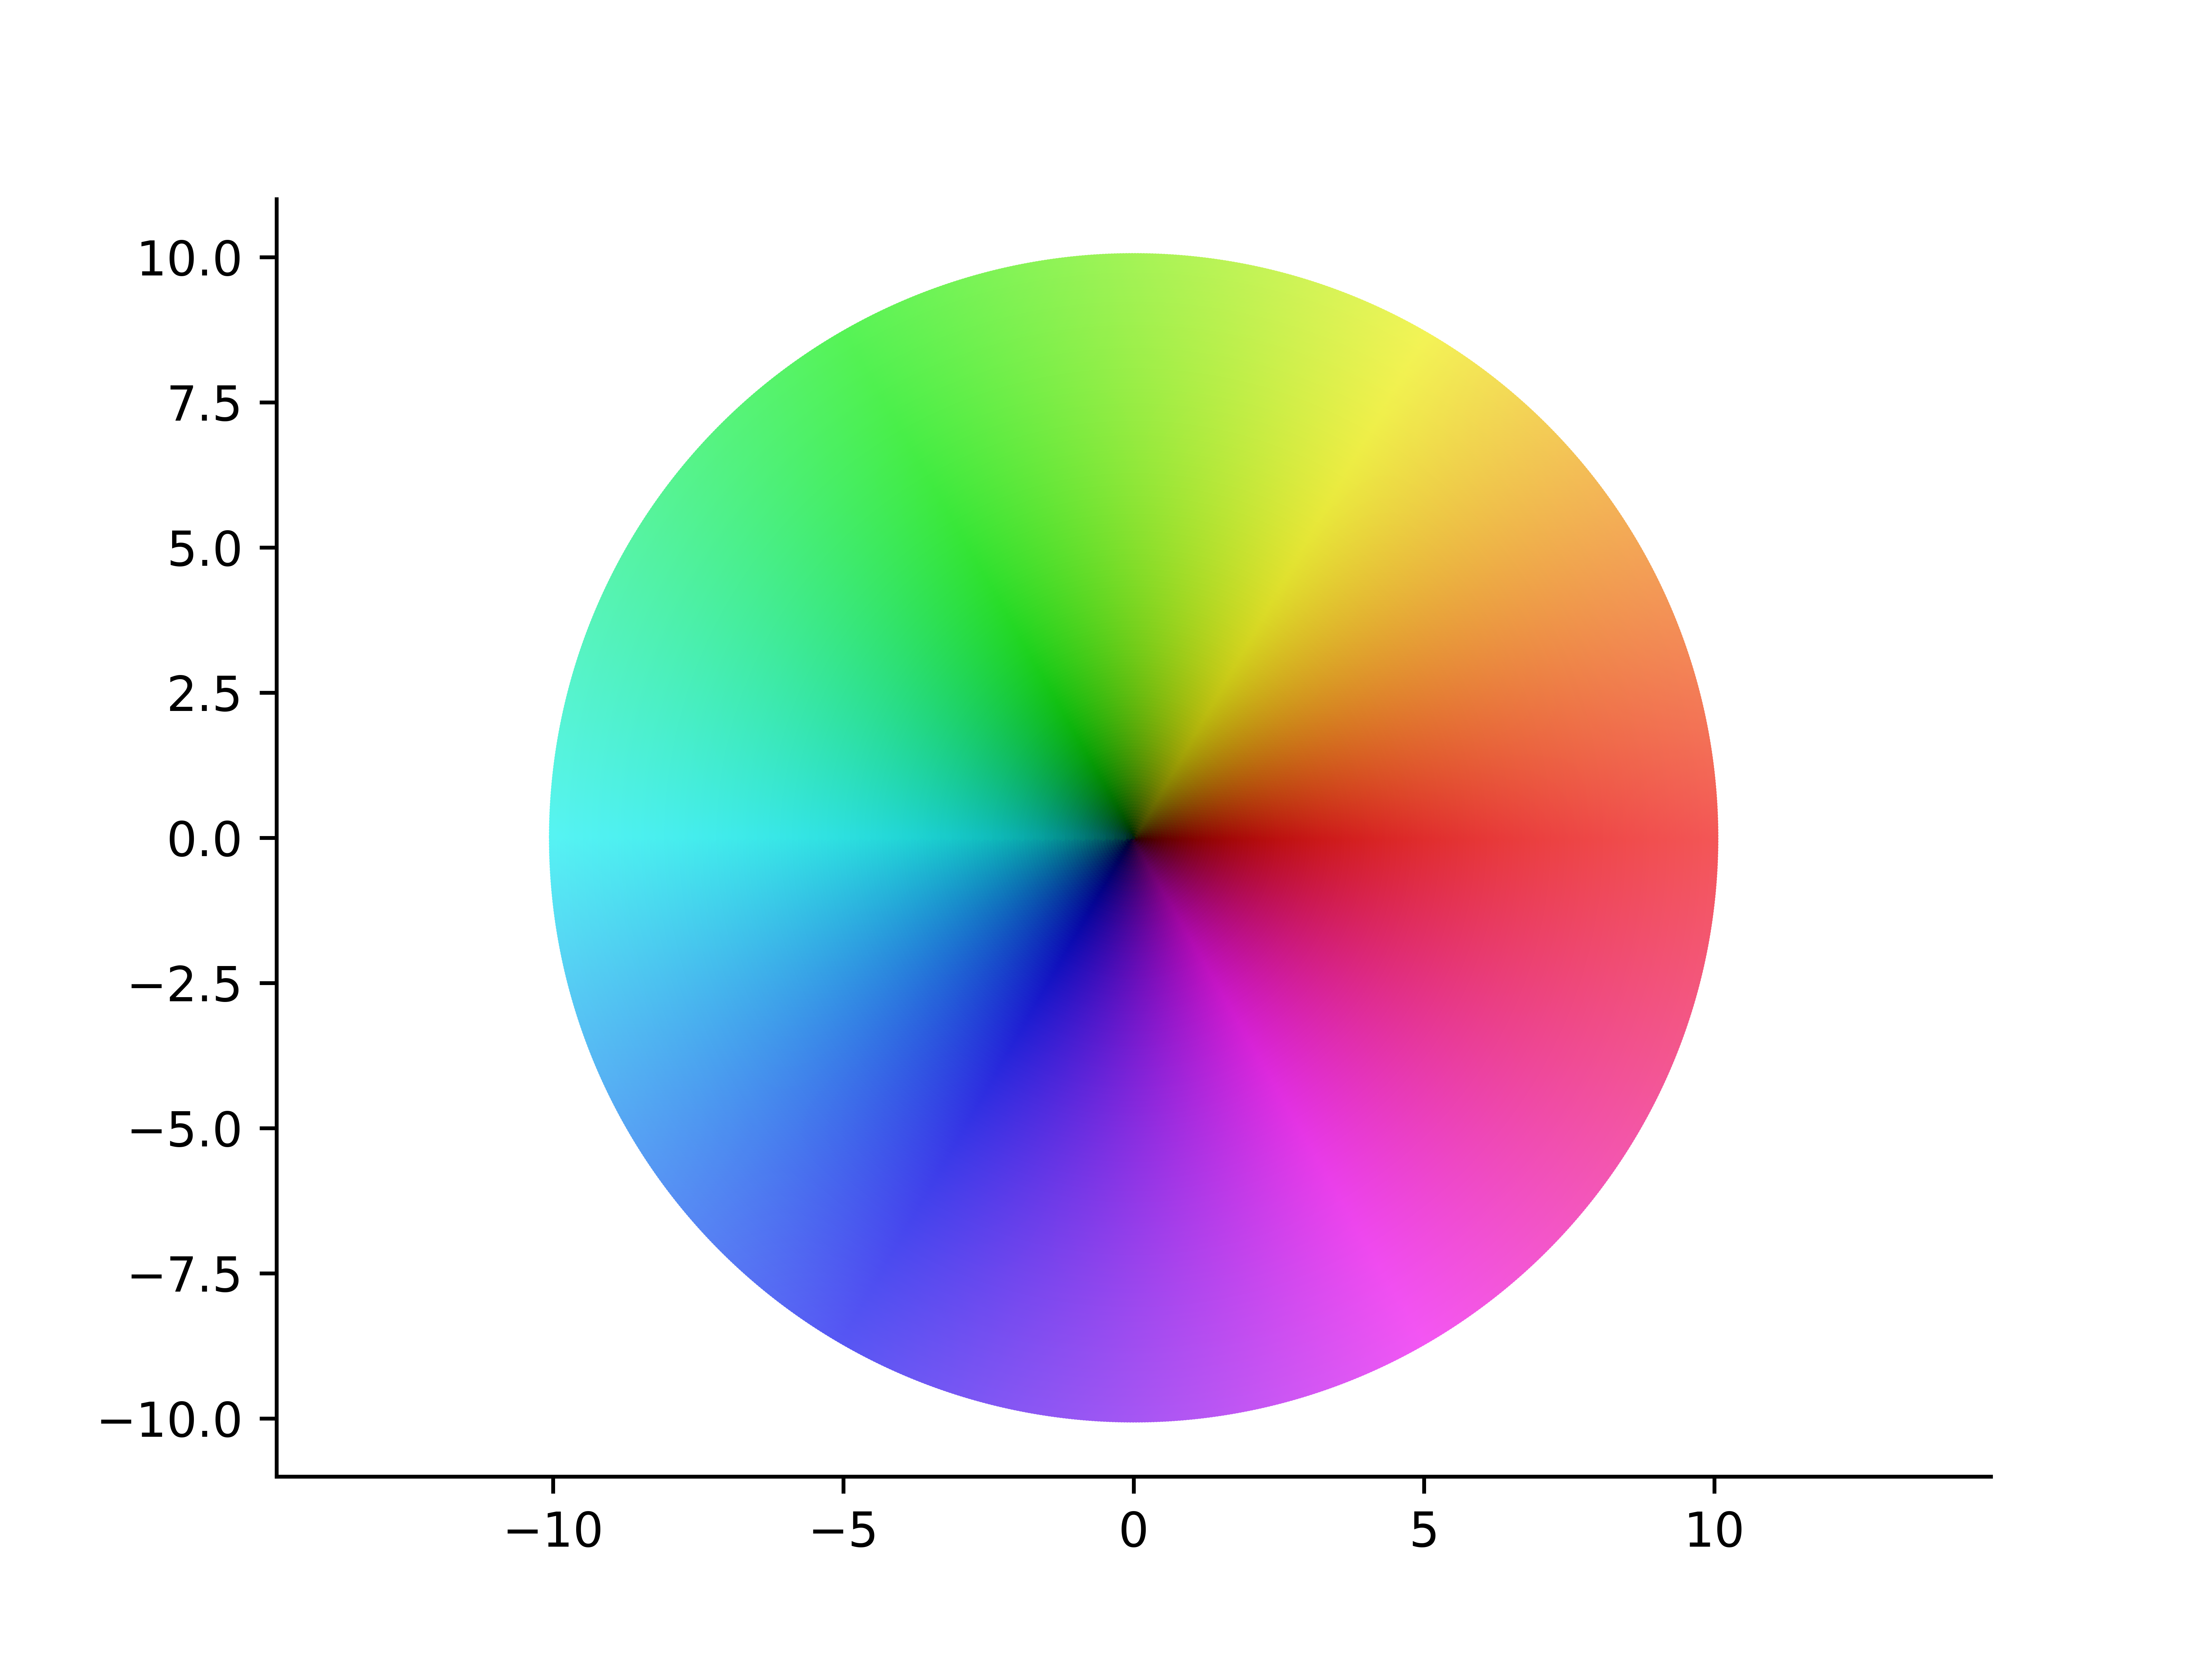
\includegraphics[width=0.7\textwidth]{../Aplicacion/z.png}
    \caption{Plano complejo coloreado}
    \label{fig:z}
\end{figure}

A continuación mostramos con unos ejemplos la gran cantidad de información que podemos extraer gracias a la representación de funciones complejas mediante la técnica de coloreado del dominio. \\

Por ejemplo, la figura \ref{fig:z^3} representa la función $f(z) = z^3$. Podemos observar que el centro del dibujo tiene un color muy oscuro. La razón es que cuando $\abs{z}$ es pequeño, $\abs{z^3}$ lo es mucho más, y por lo tanto el color asignado a $z^3$ es muy oscuro. También podemos ver que los colores se vuelven muy claros conforme nos vamos alejando del centro. Esto ocurre porque cuando $z$ es de módulo grande, también lo es $z^3$, y por consiguiente el color correspondiente es muy claro. \\

\begin{figure}[!htbp]
    \centering
    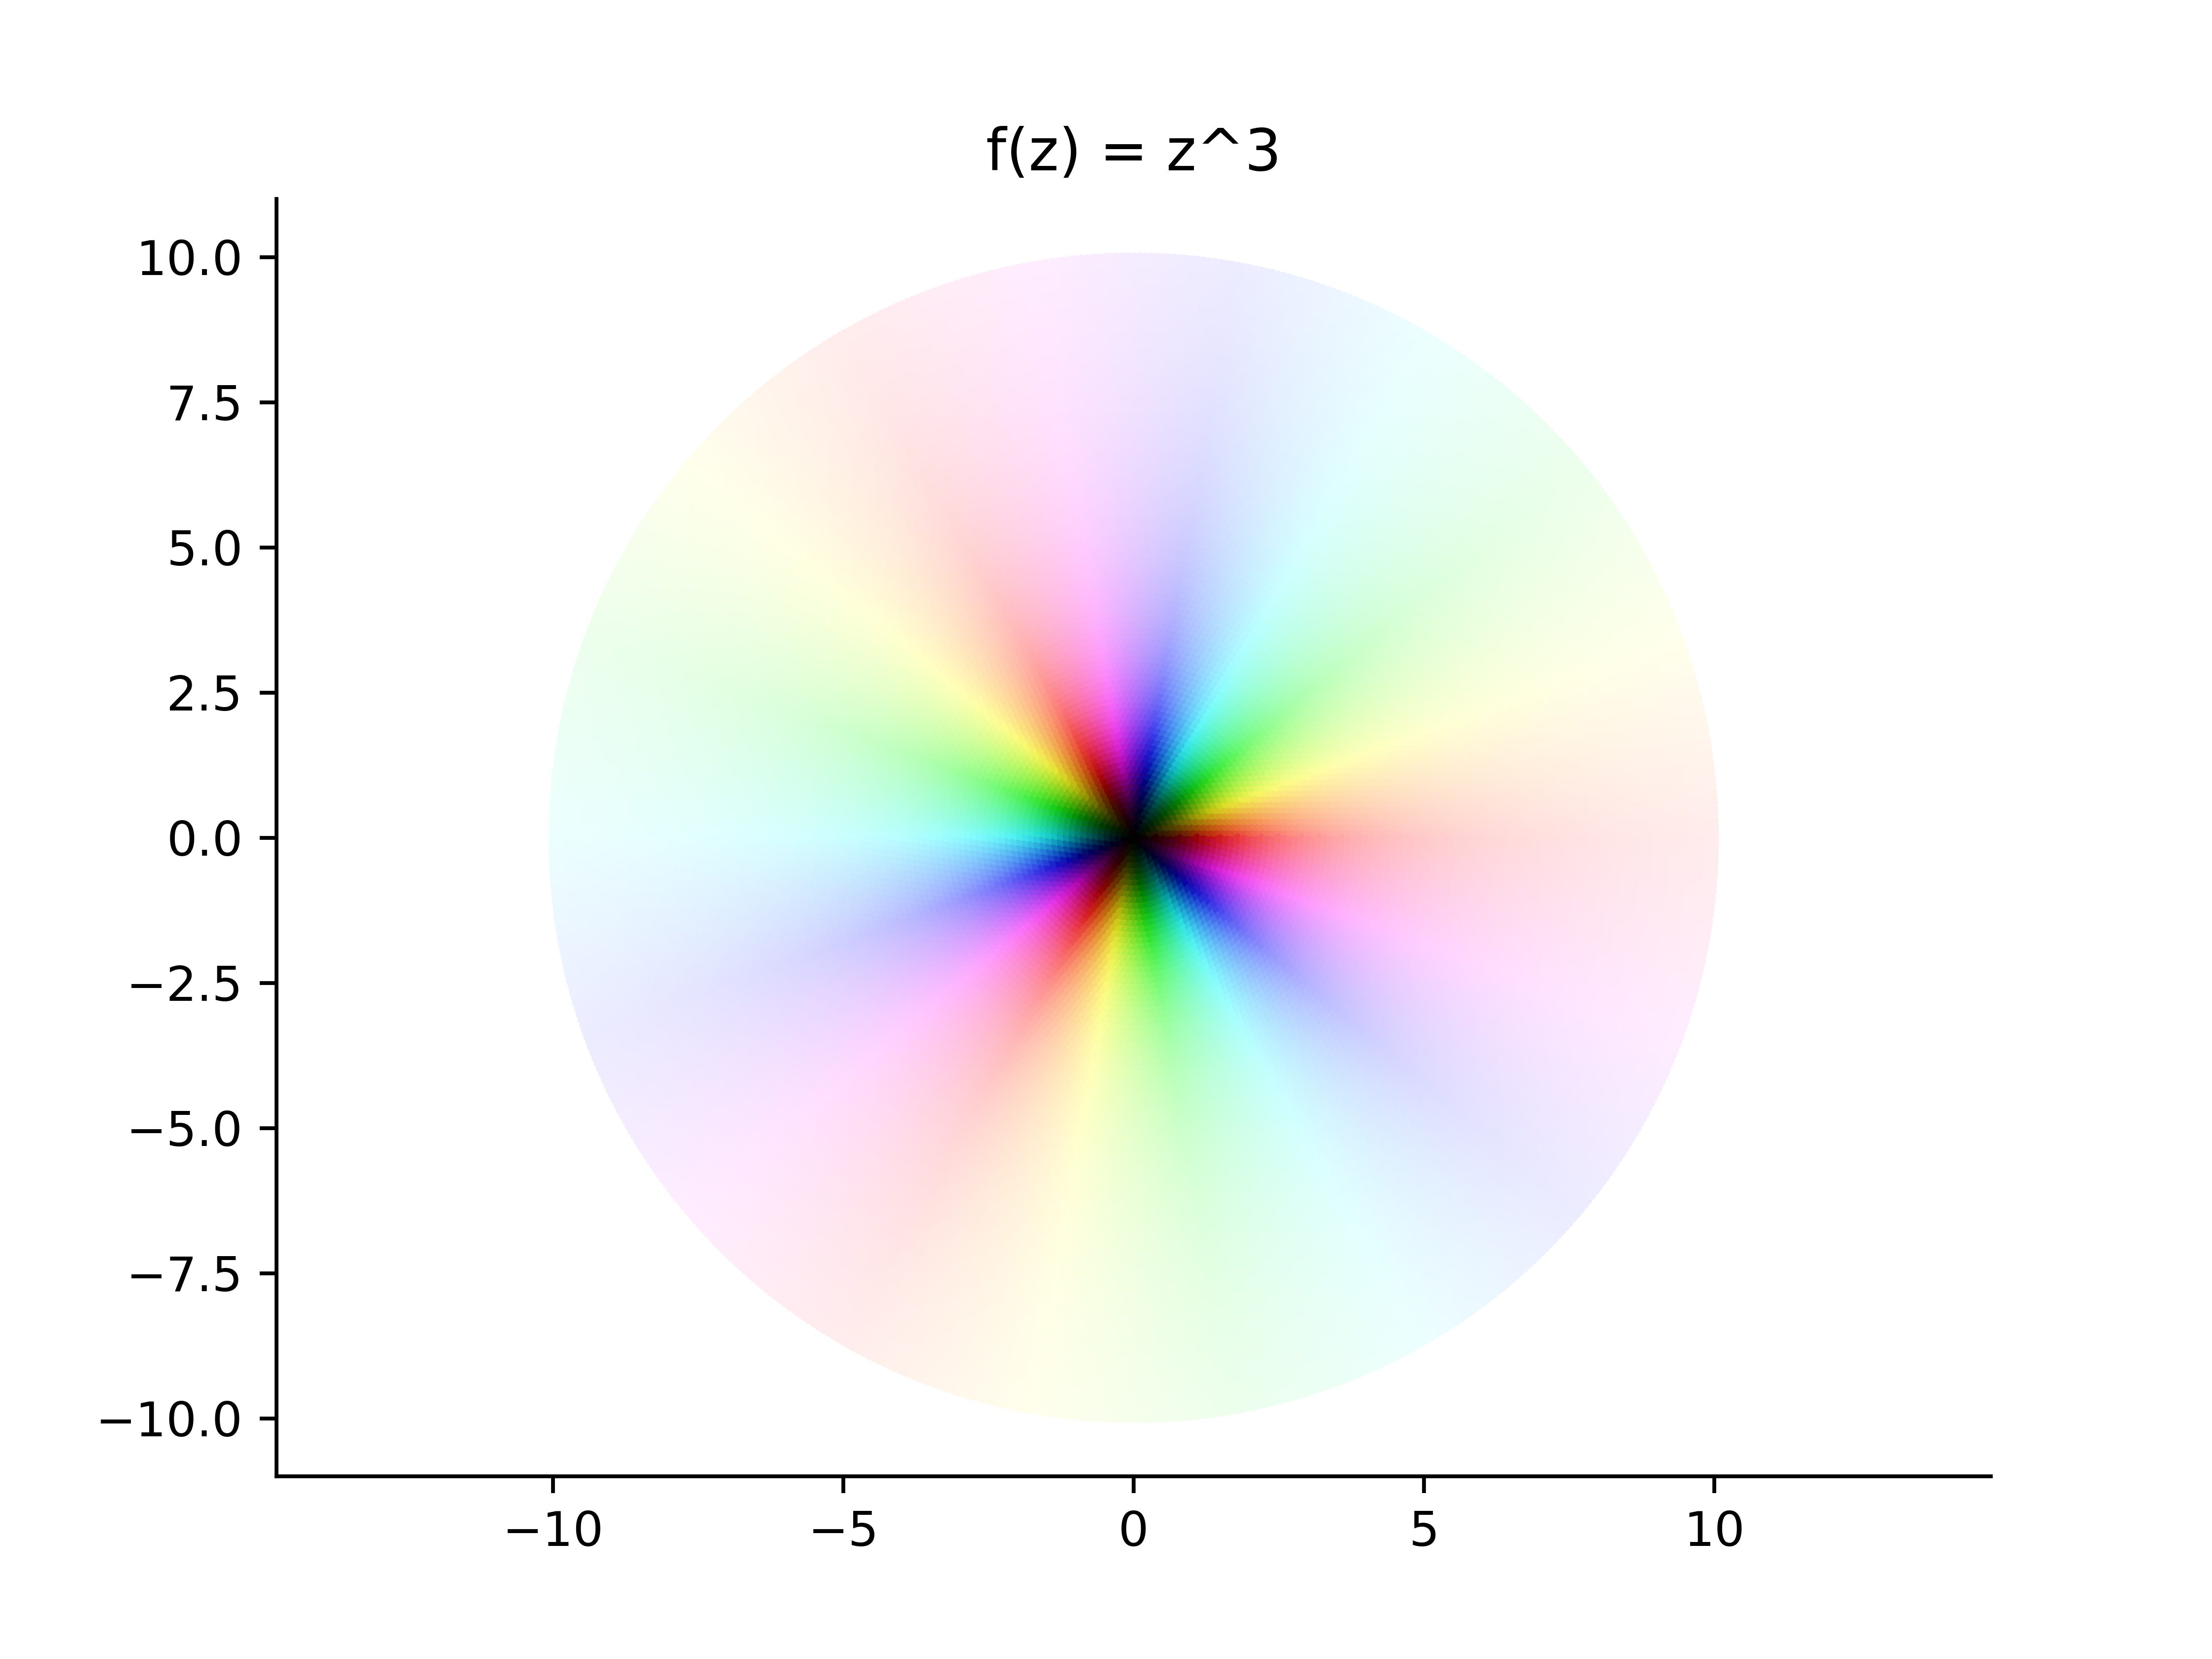
\includegraphics[width=0.7\textwidth]{../Aplicacion/z^3.png}
    \caption{Representación de la función $f(z) = z^3$.}
    \label{fig:z^3}
\end{figure}

Puesto que el color asignado al número $0$ es el negro, sabemos que las raíces del polinomio se corresponden con los puntos negros. En el caso que nos ocupa, el $0$ es una raíz triple de la función y se puede observar en que los colores del círculo cromático la envuelven tres veces. \\

Por último cuando avanzamos en el sentido contrario a las agujas del reloj, pasamos por los colores del círculo cromático $3$ veces. Esto muestra el hecho de que el argumento de $z^3$ es tres veces el argumento de $z$, y por lo tanto la imagen de un círculo centrado en el origen bajo la función cúbica se envuelve alrededor del origen tres veces. Esto se explica porque para cada número de módulo $s=r^3$ encontramos tres raíces distintas de módulo $r$. Si representamos la función $f(z)=e^{z^3}-1$, observamos una imagen que, cerca del $0$, es análoga a la anterior, pues tiene un cero triple en $z=0$. La figura \ref{fig:e^(z^3)-1} muestra este último ejemplo. \\

\begin{figure}[!htbp]
    \centering
    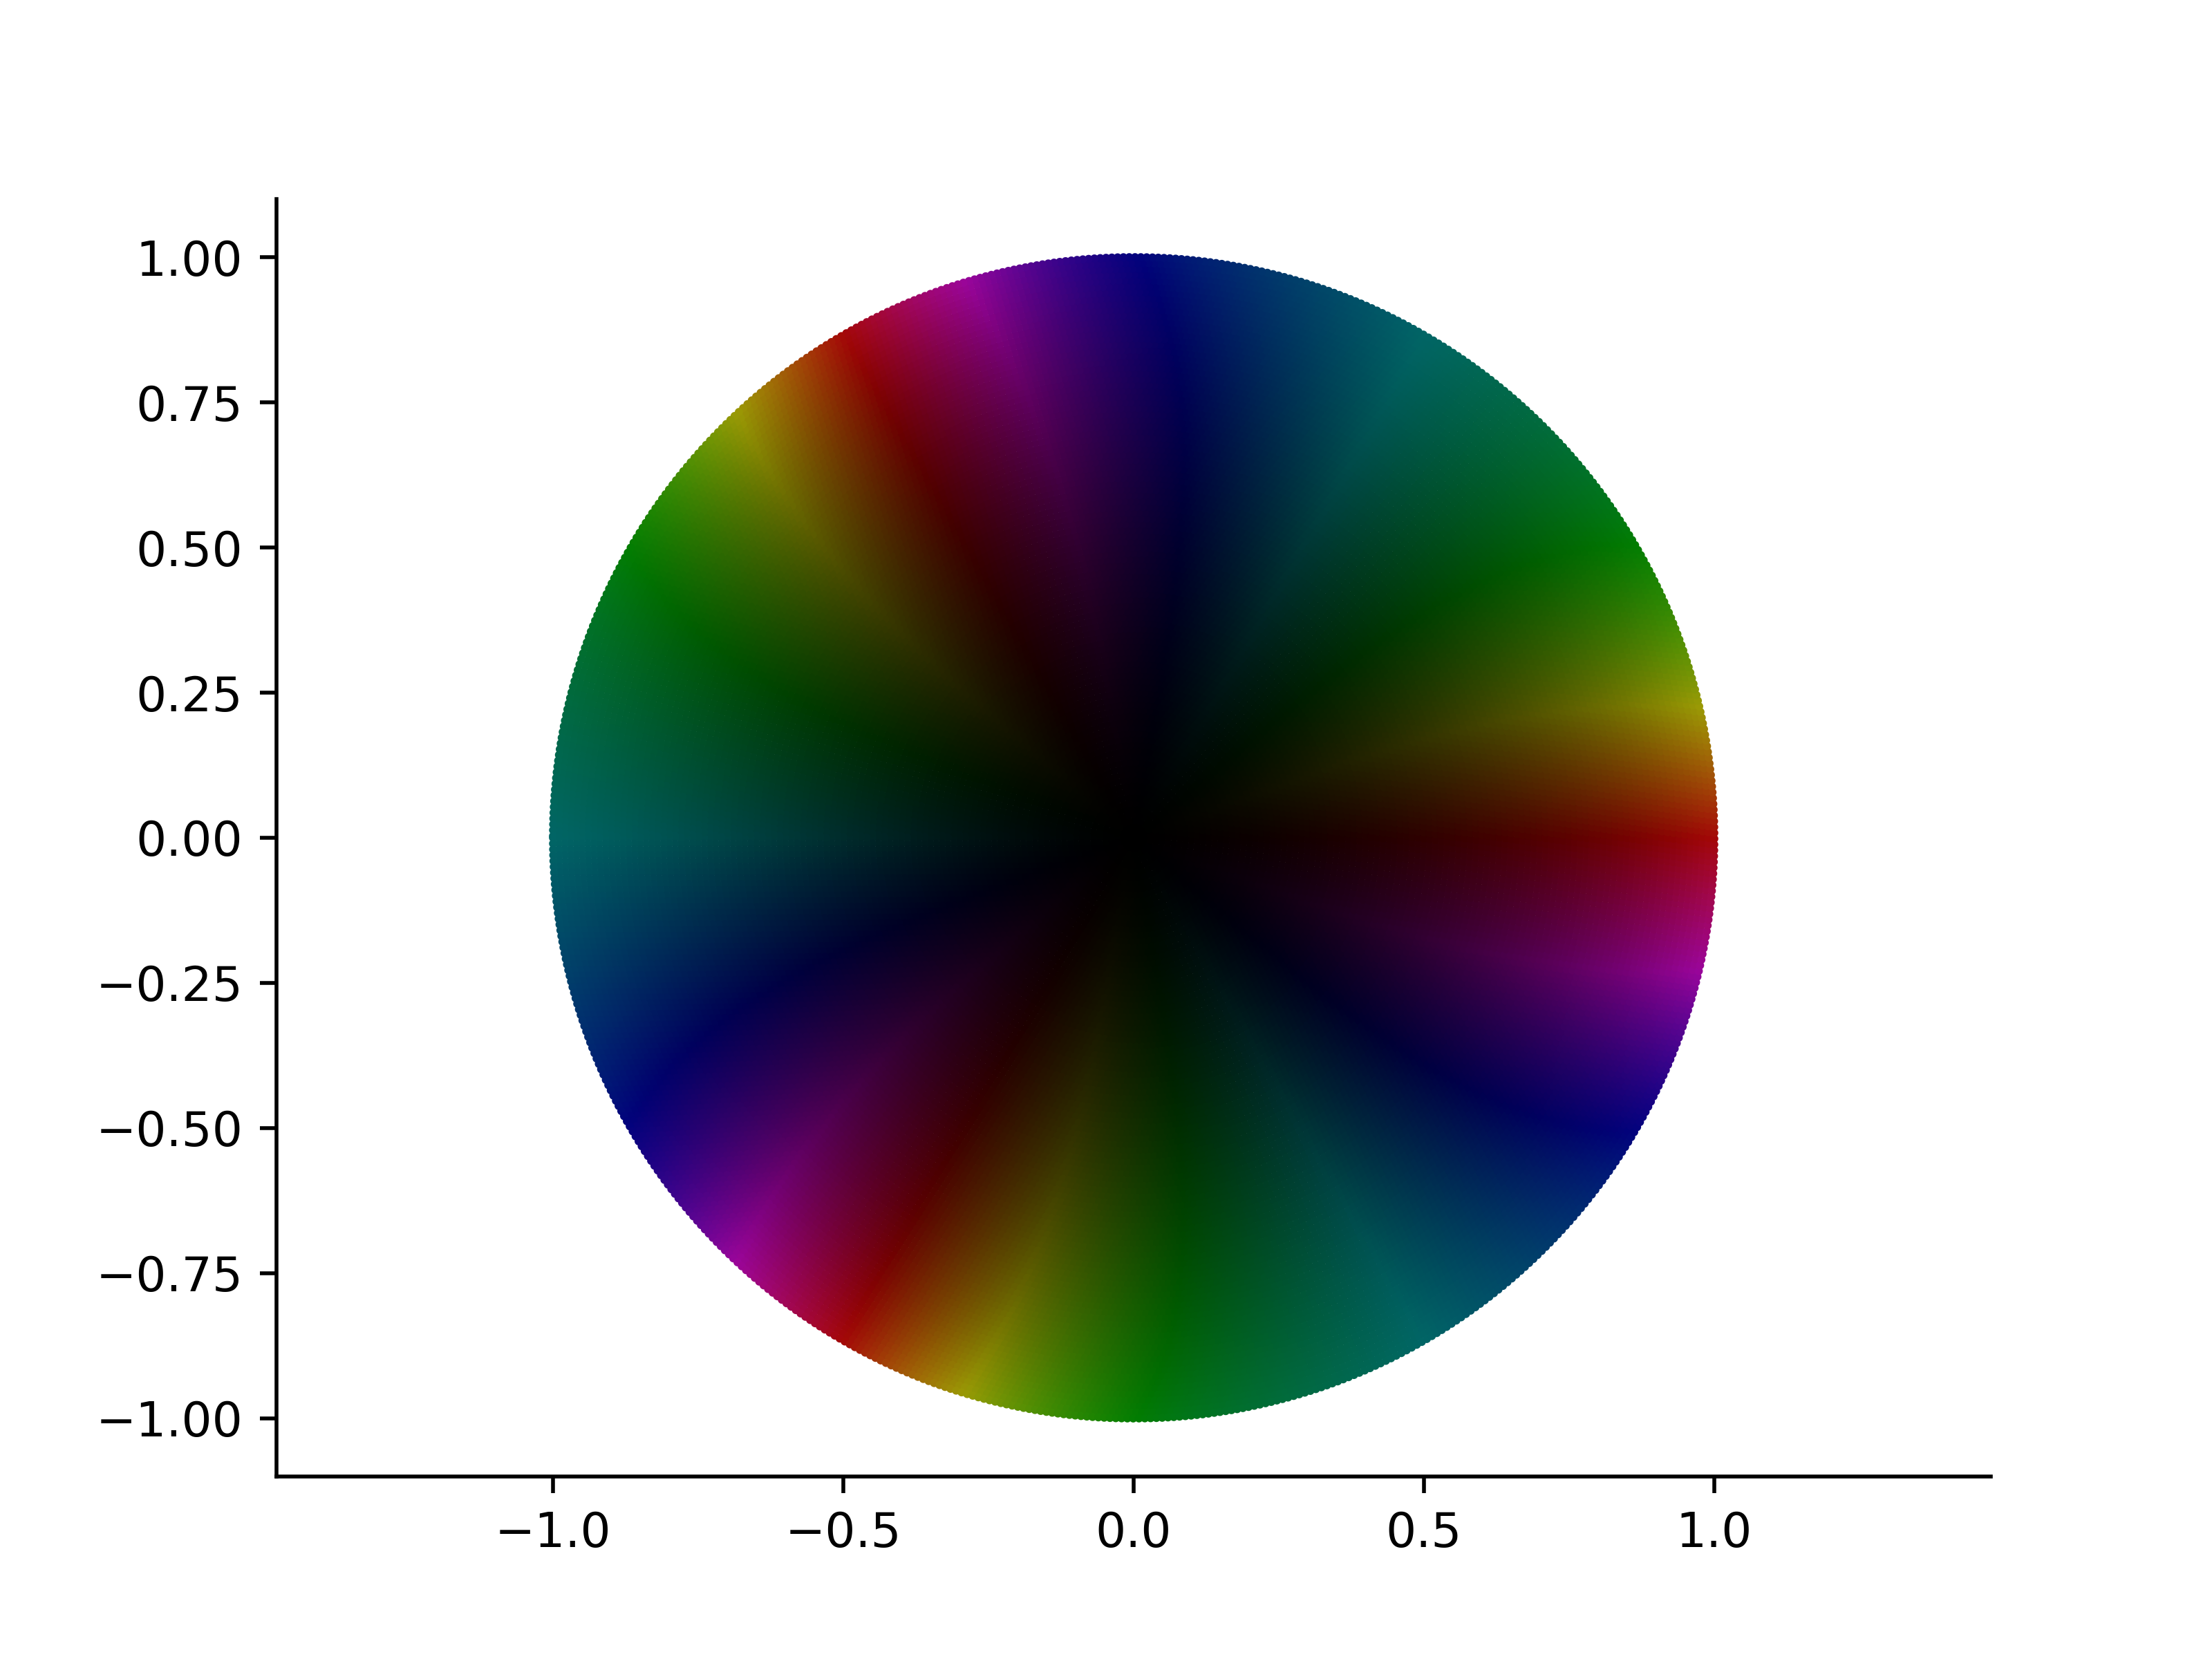
\includegraphics[width=0.7\textwidth]{../Aplicacion/e^(z^3)-1.png}
    \caption{Representación de la función $f(z) = e^{z^3}-1$.}
    \label{fig:e^(z^3)-1}
\end{figure}

La figura \ref{fig:1/z} muestra la representación de la función $f(z) = \frac{1}{z}$ con la técnica del coloreado. En este caso, el color que se le ha asignado al $0$ es blanco, lo que indica que $\frac{1}{z}$ tiende a infinito cuando $z$ tiende a $0$. Es decir, nos encontramos ante un polo de la función. Podemos observar que en el origen se envuelven los colores del círculo cromático una única vez en sentido contrario, lo que indica que se trata de un polo simple. La función $\frac{\cos z}{z}$, por ejemplo, también tiene un cero simple en $z=0$ y un representación análoga a $\frac{1}{z}$ en un entorno del origen. \\

\begin{figure}[!htbp]
    \centering
    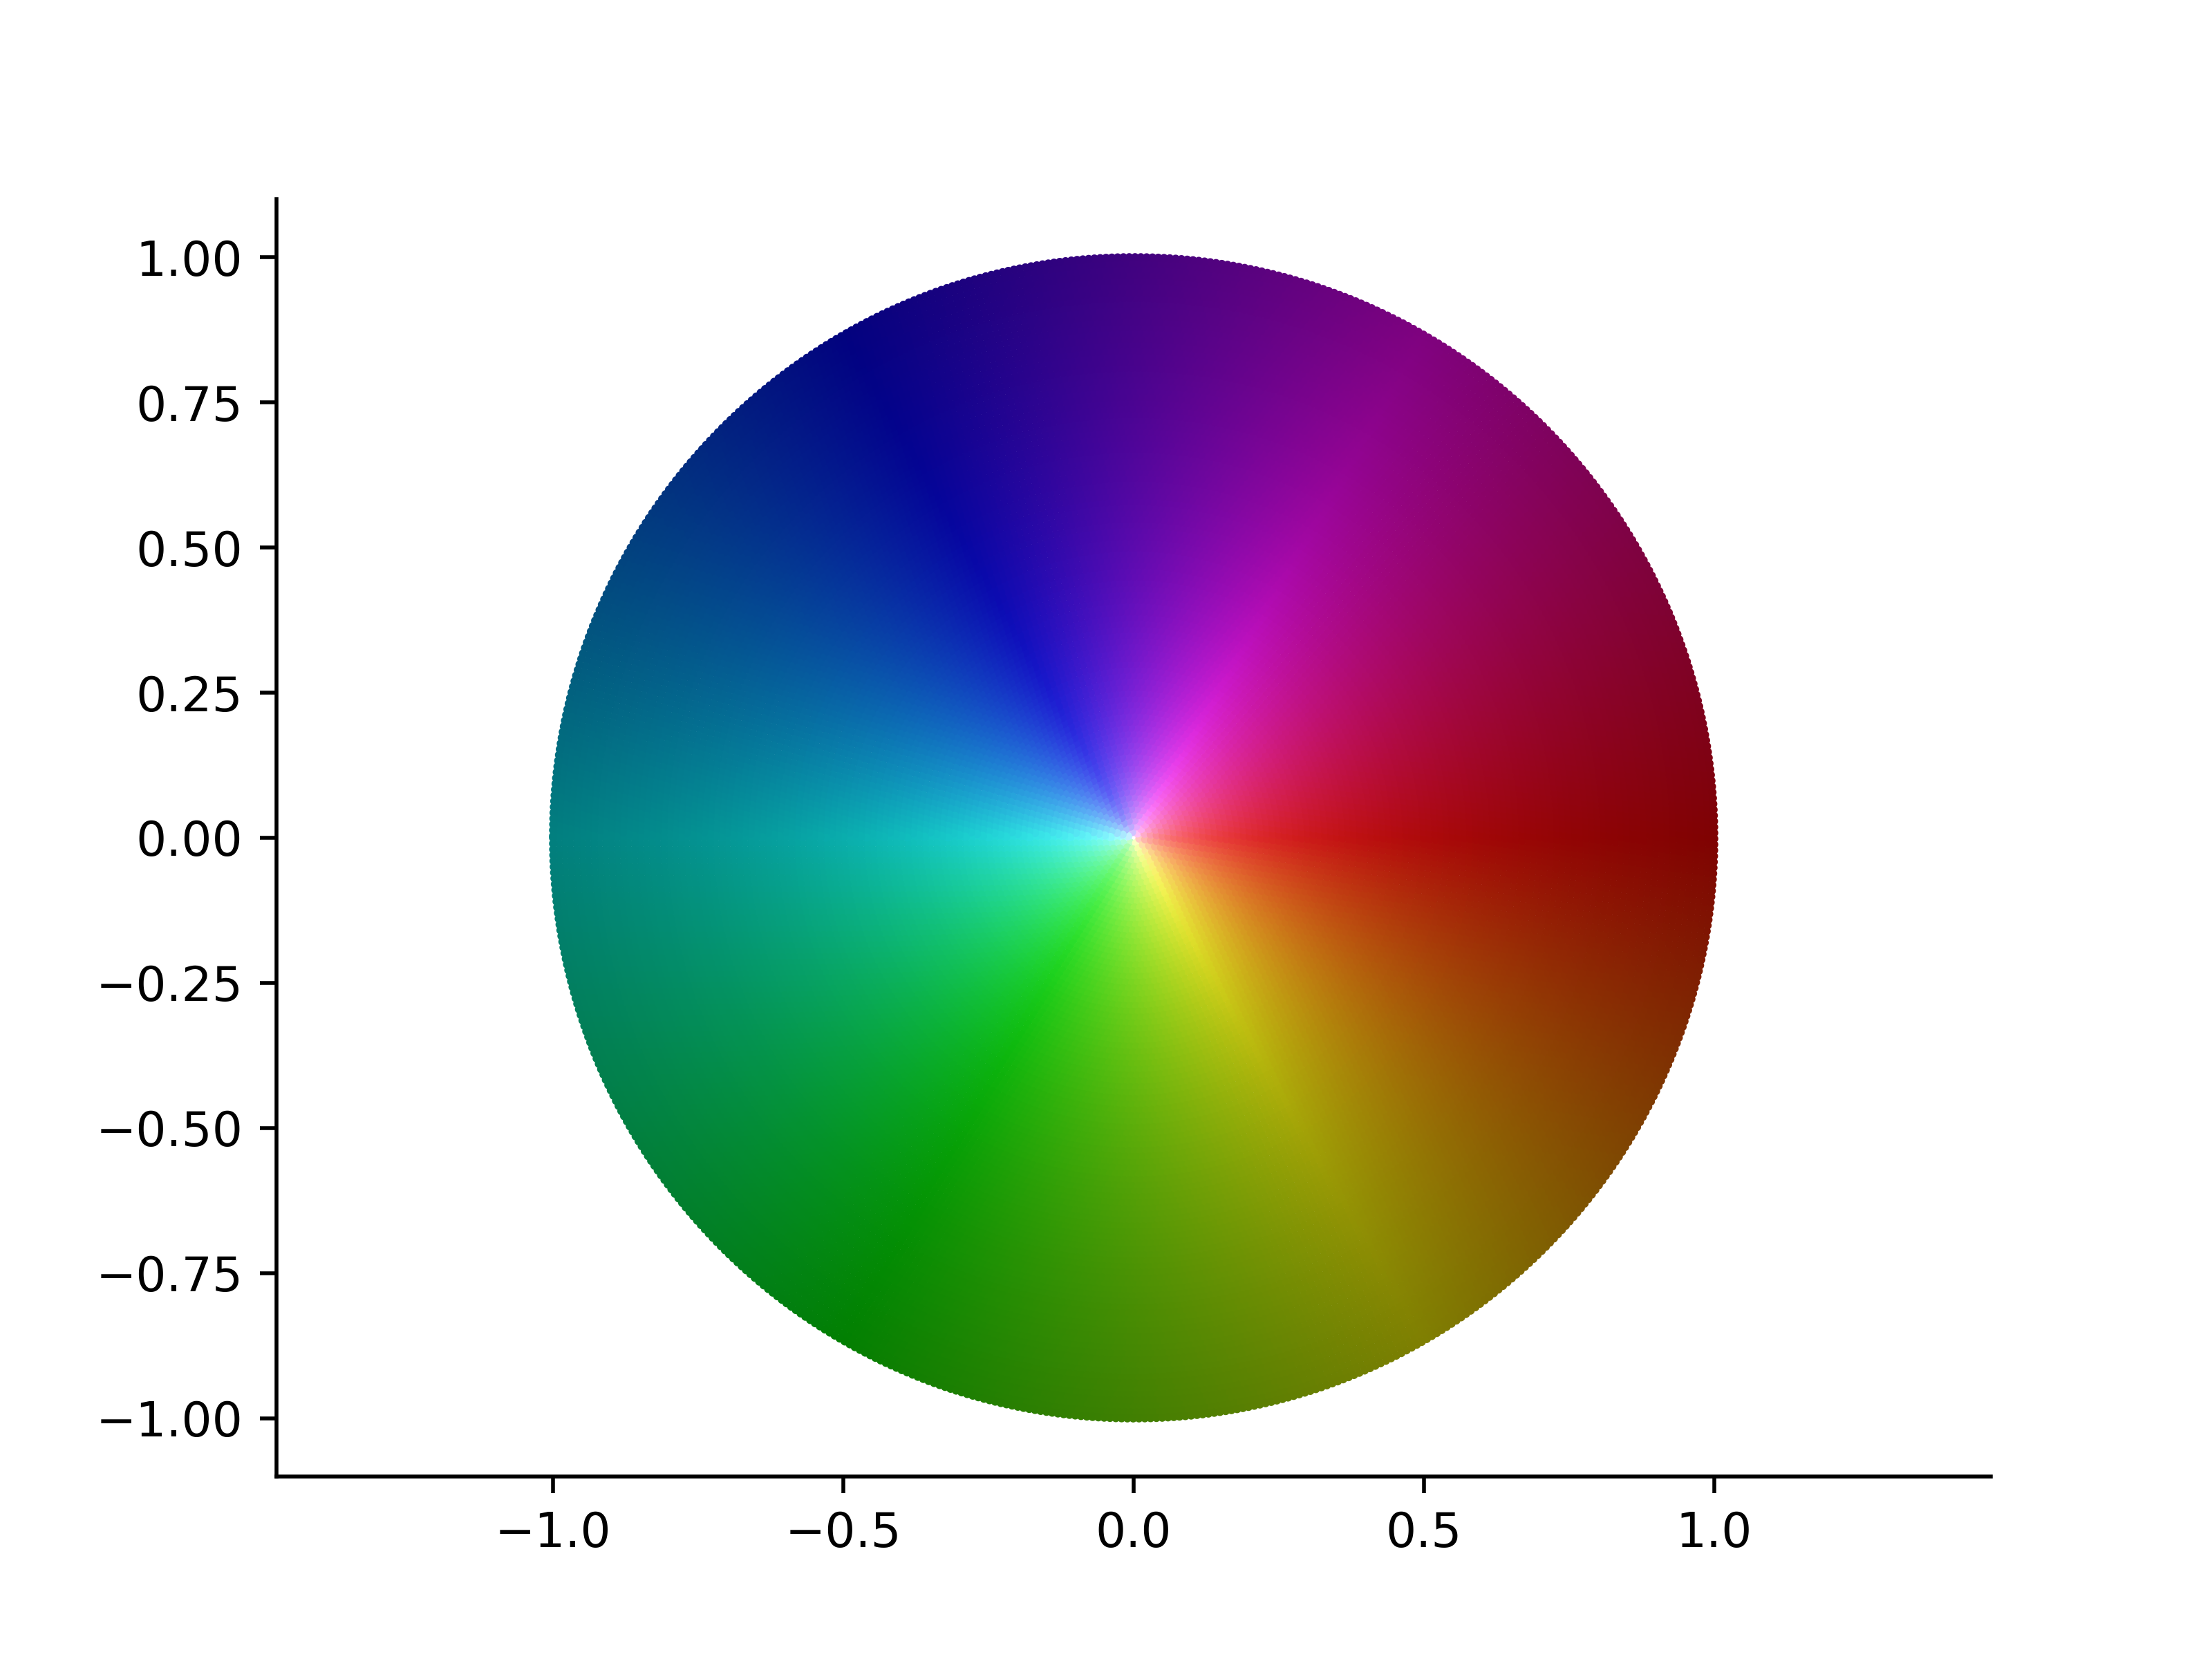
\includegraphics[width=0.7\textwidth]{../Aplicacion/1:z.png}
    \caption{Representación de la función $f(z) = \frac{1}{z}$.}
    \label{fig:1/z}
\end{figure}

Las funciones $e^z$ y $\sen(z)$ van a ilustrar el caso de las funciones periódicas. Se puede ver su representación en las figuras \ref{fig:e^z} y \ref{fig:sen(z)}, respectivamente. Observamos que en el caso de la exponencial ahora los colores van cambiando conforme avanzamos verticalmente. Si escribimos $z = x + iy$, entonces $e^z = e^{x+i y} = e^x e^{i y}$. Por lo que $y$, la parte imaginaria de $z$, determina el argumento y, por tanto, el color. Queda claro que el argumento es periódico de período $2 \pi$ en la dirección imaginaria. \\

\begin{figure}[!htbp]
    \centering
    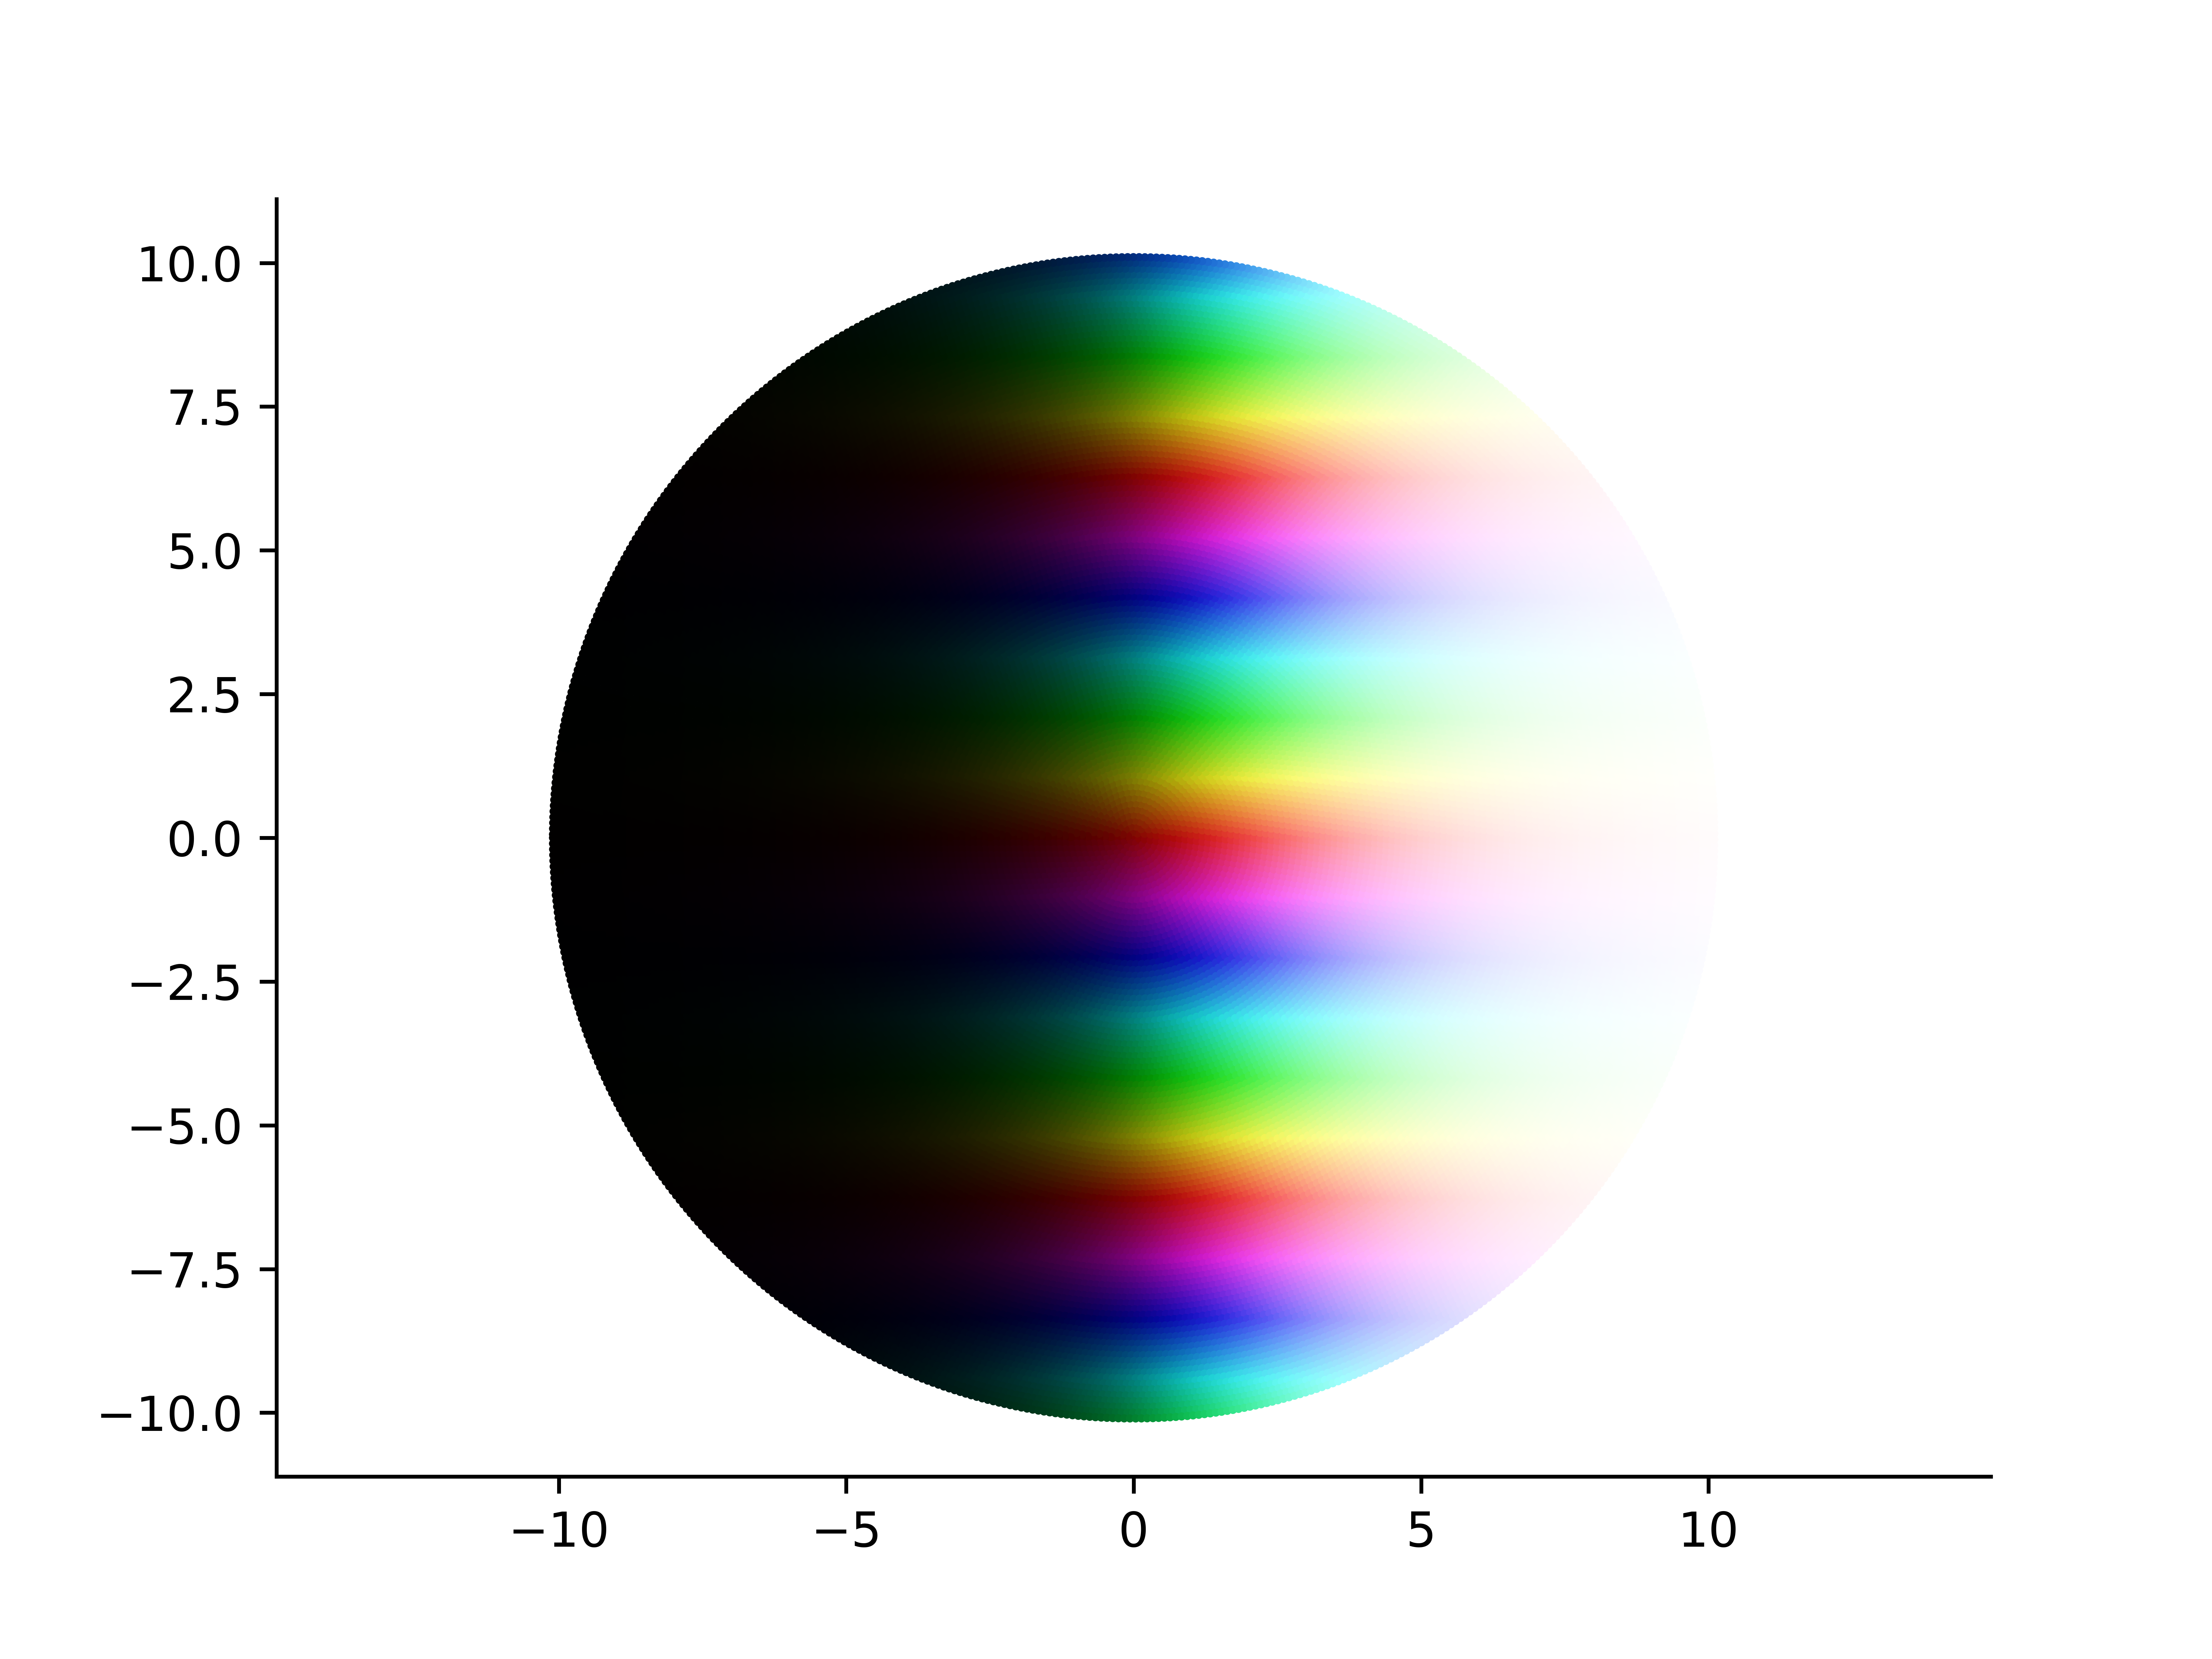
\includegraphics[width=0.7\textwidth]{../Aplicacion/e^z.png}
    \caption{Representación de la función $f(z) = e^z$.}
    \label{fig:e^z}
\end{figure}

\begin{figure}[!htbp]
    \centering
    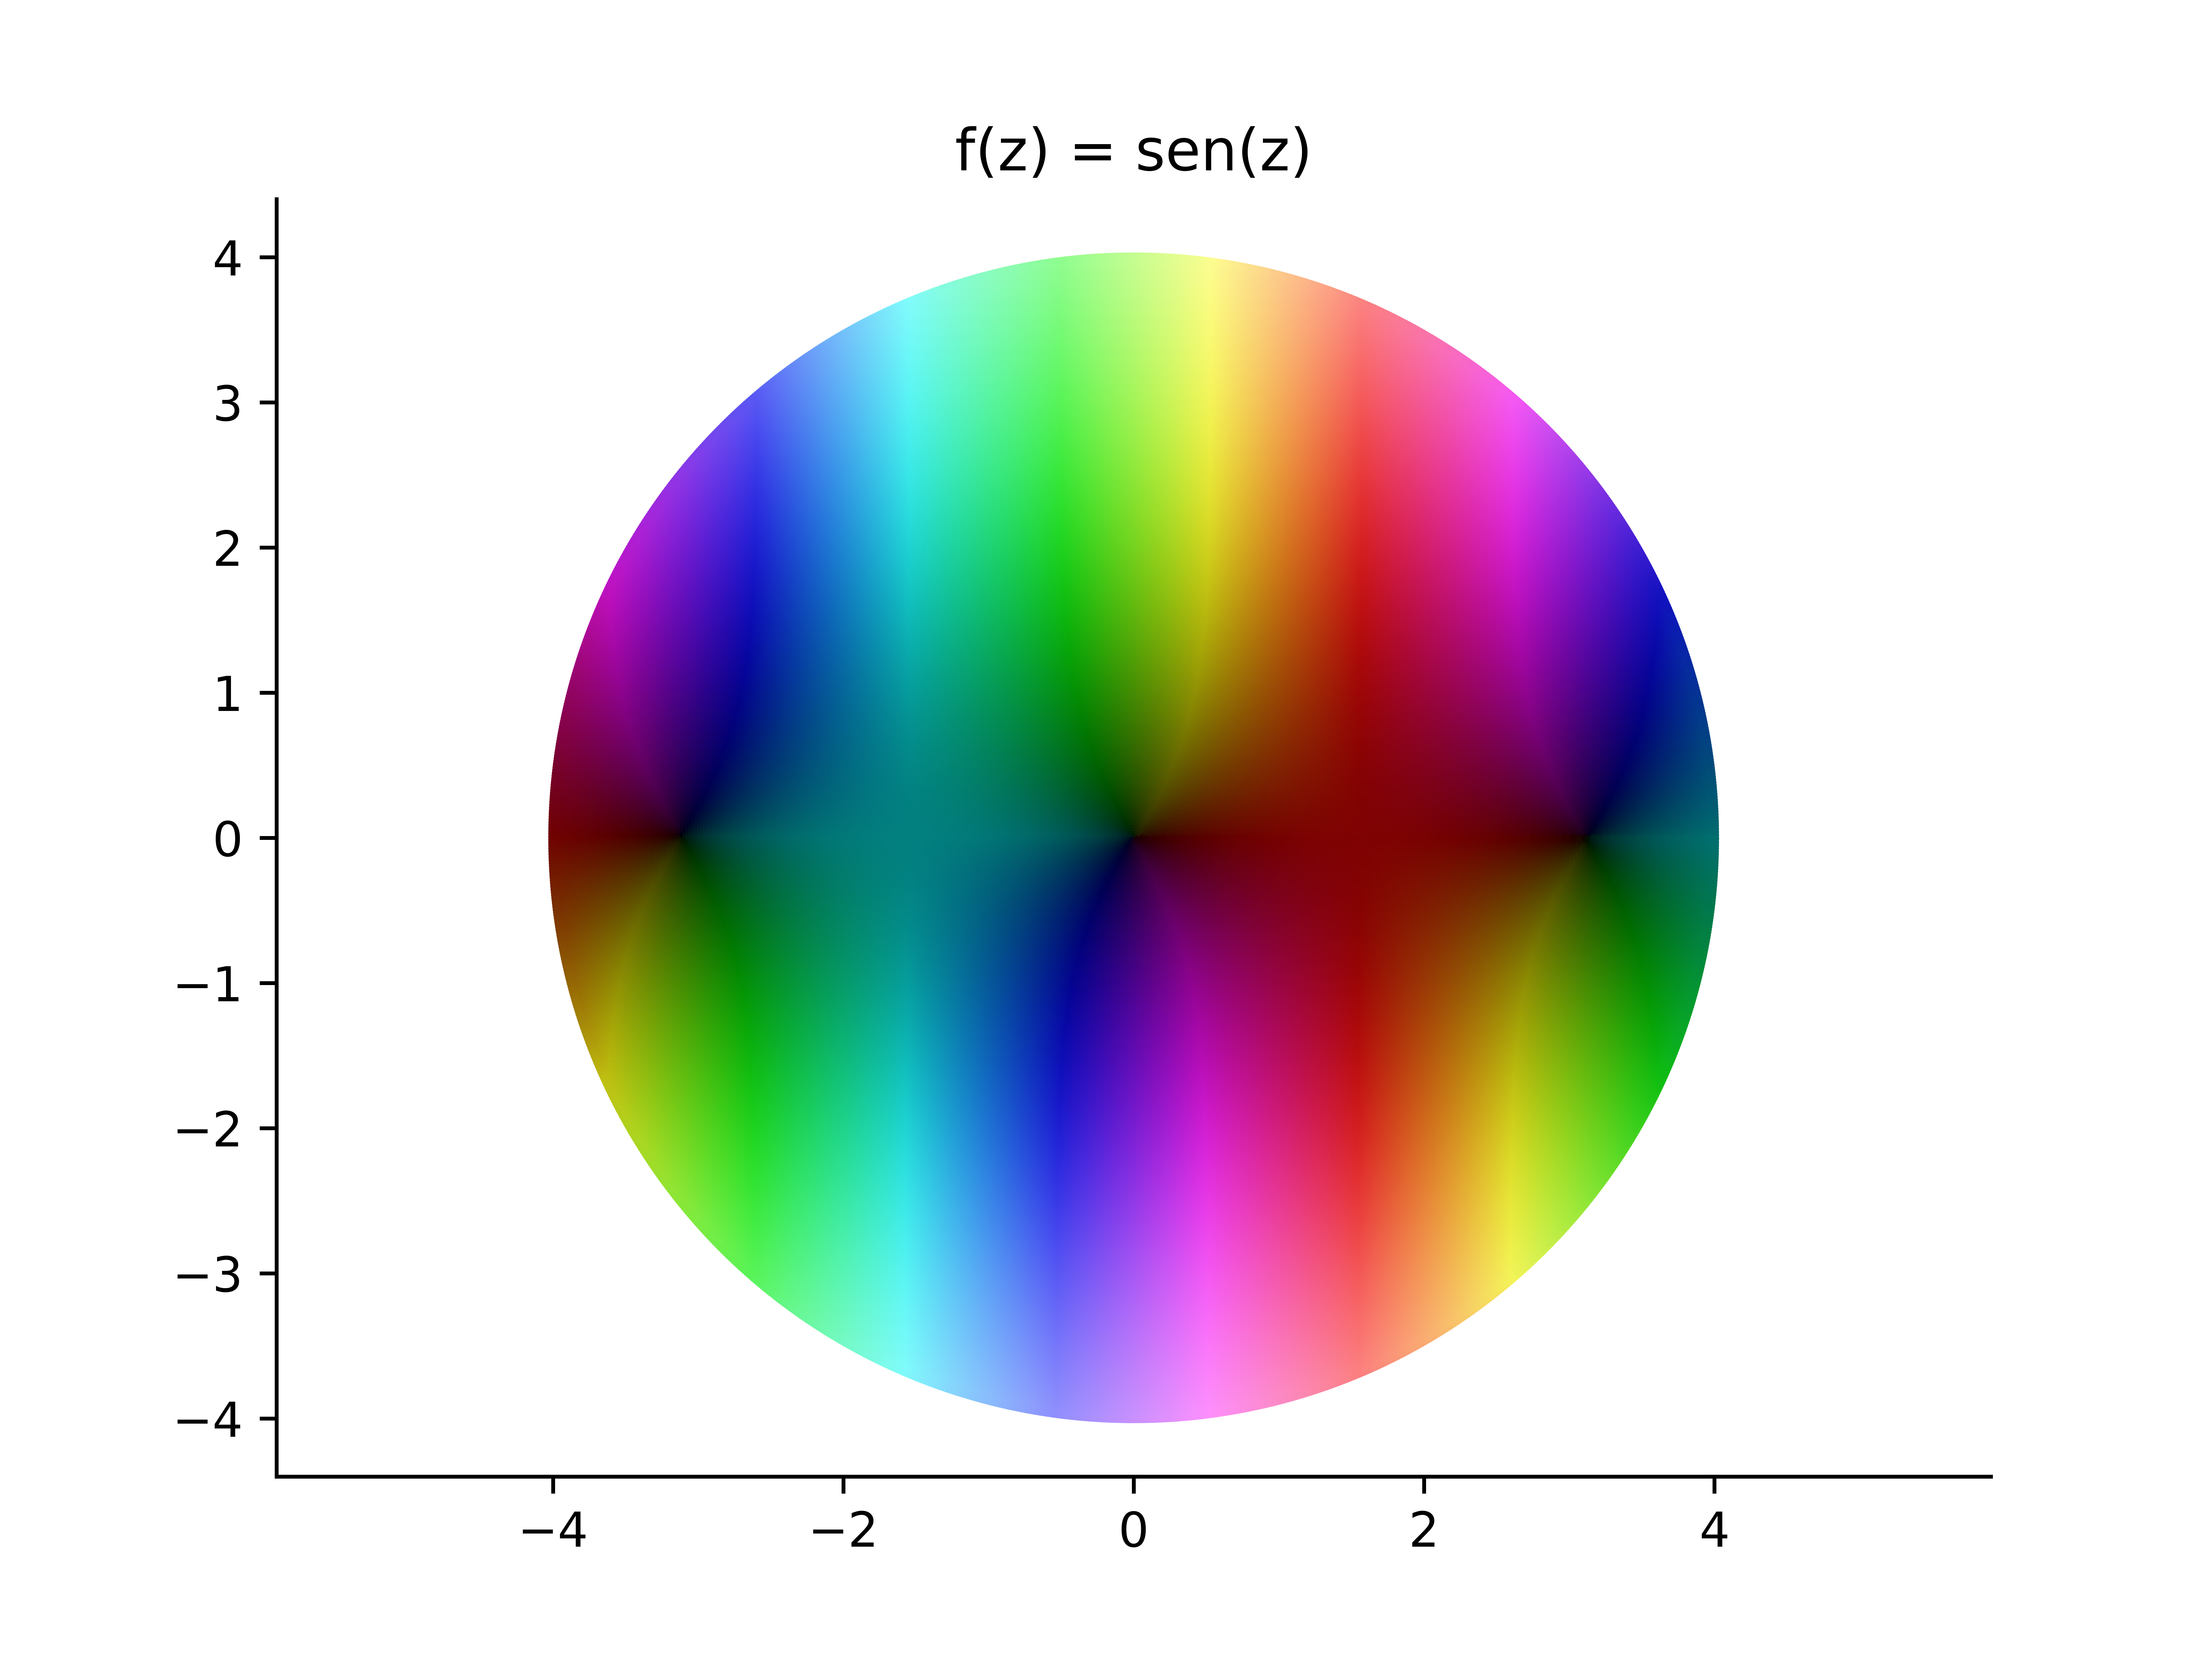
\includegraphics[width=0.7\textwidth]{../Aplicacion/sen(z).png}
    \caption{Representación de la función $f(z) = \sen(z)$.}
    \label{fig:sen(z)}
\end{figure}

La figura \ref{fig:log(z)} representa la función $\log(z)$, una función no continua. Al haber discontinuidad en una semirrecta -porque no se puede definir un argumento continuo-, queda muy patente que la técnica del coloreado permite detectar estas discontinuidades. También es muy drástico cómo se ven las singularidades esenciales, por ejemplo, en $z = 0$ para $\sen(\frac{1}{z})$. En el capítulo \ref{cap:ejemplos} se mostrará mediante un ejemplo cómo se representan las singularidades esenciales con la técnica del coloreado. \\

\begin{figure}[!htbp]
    \centering
    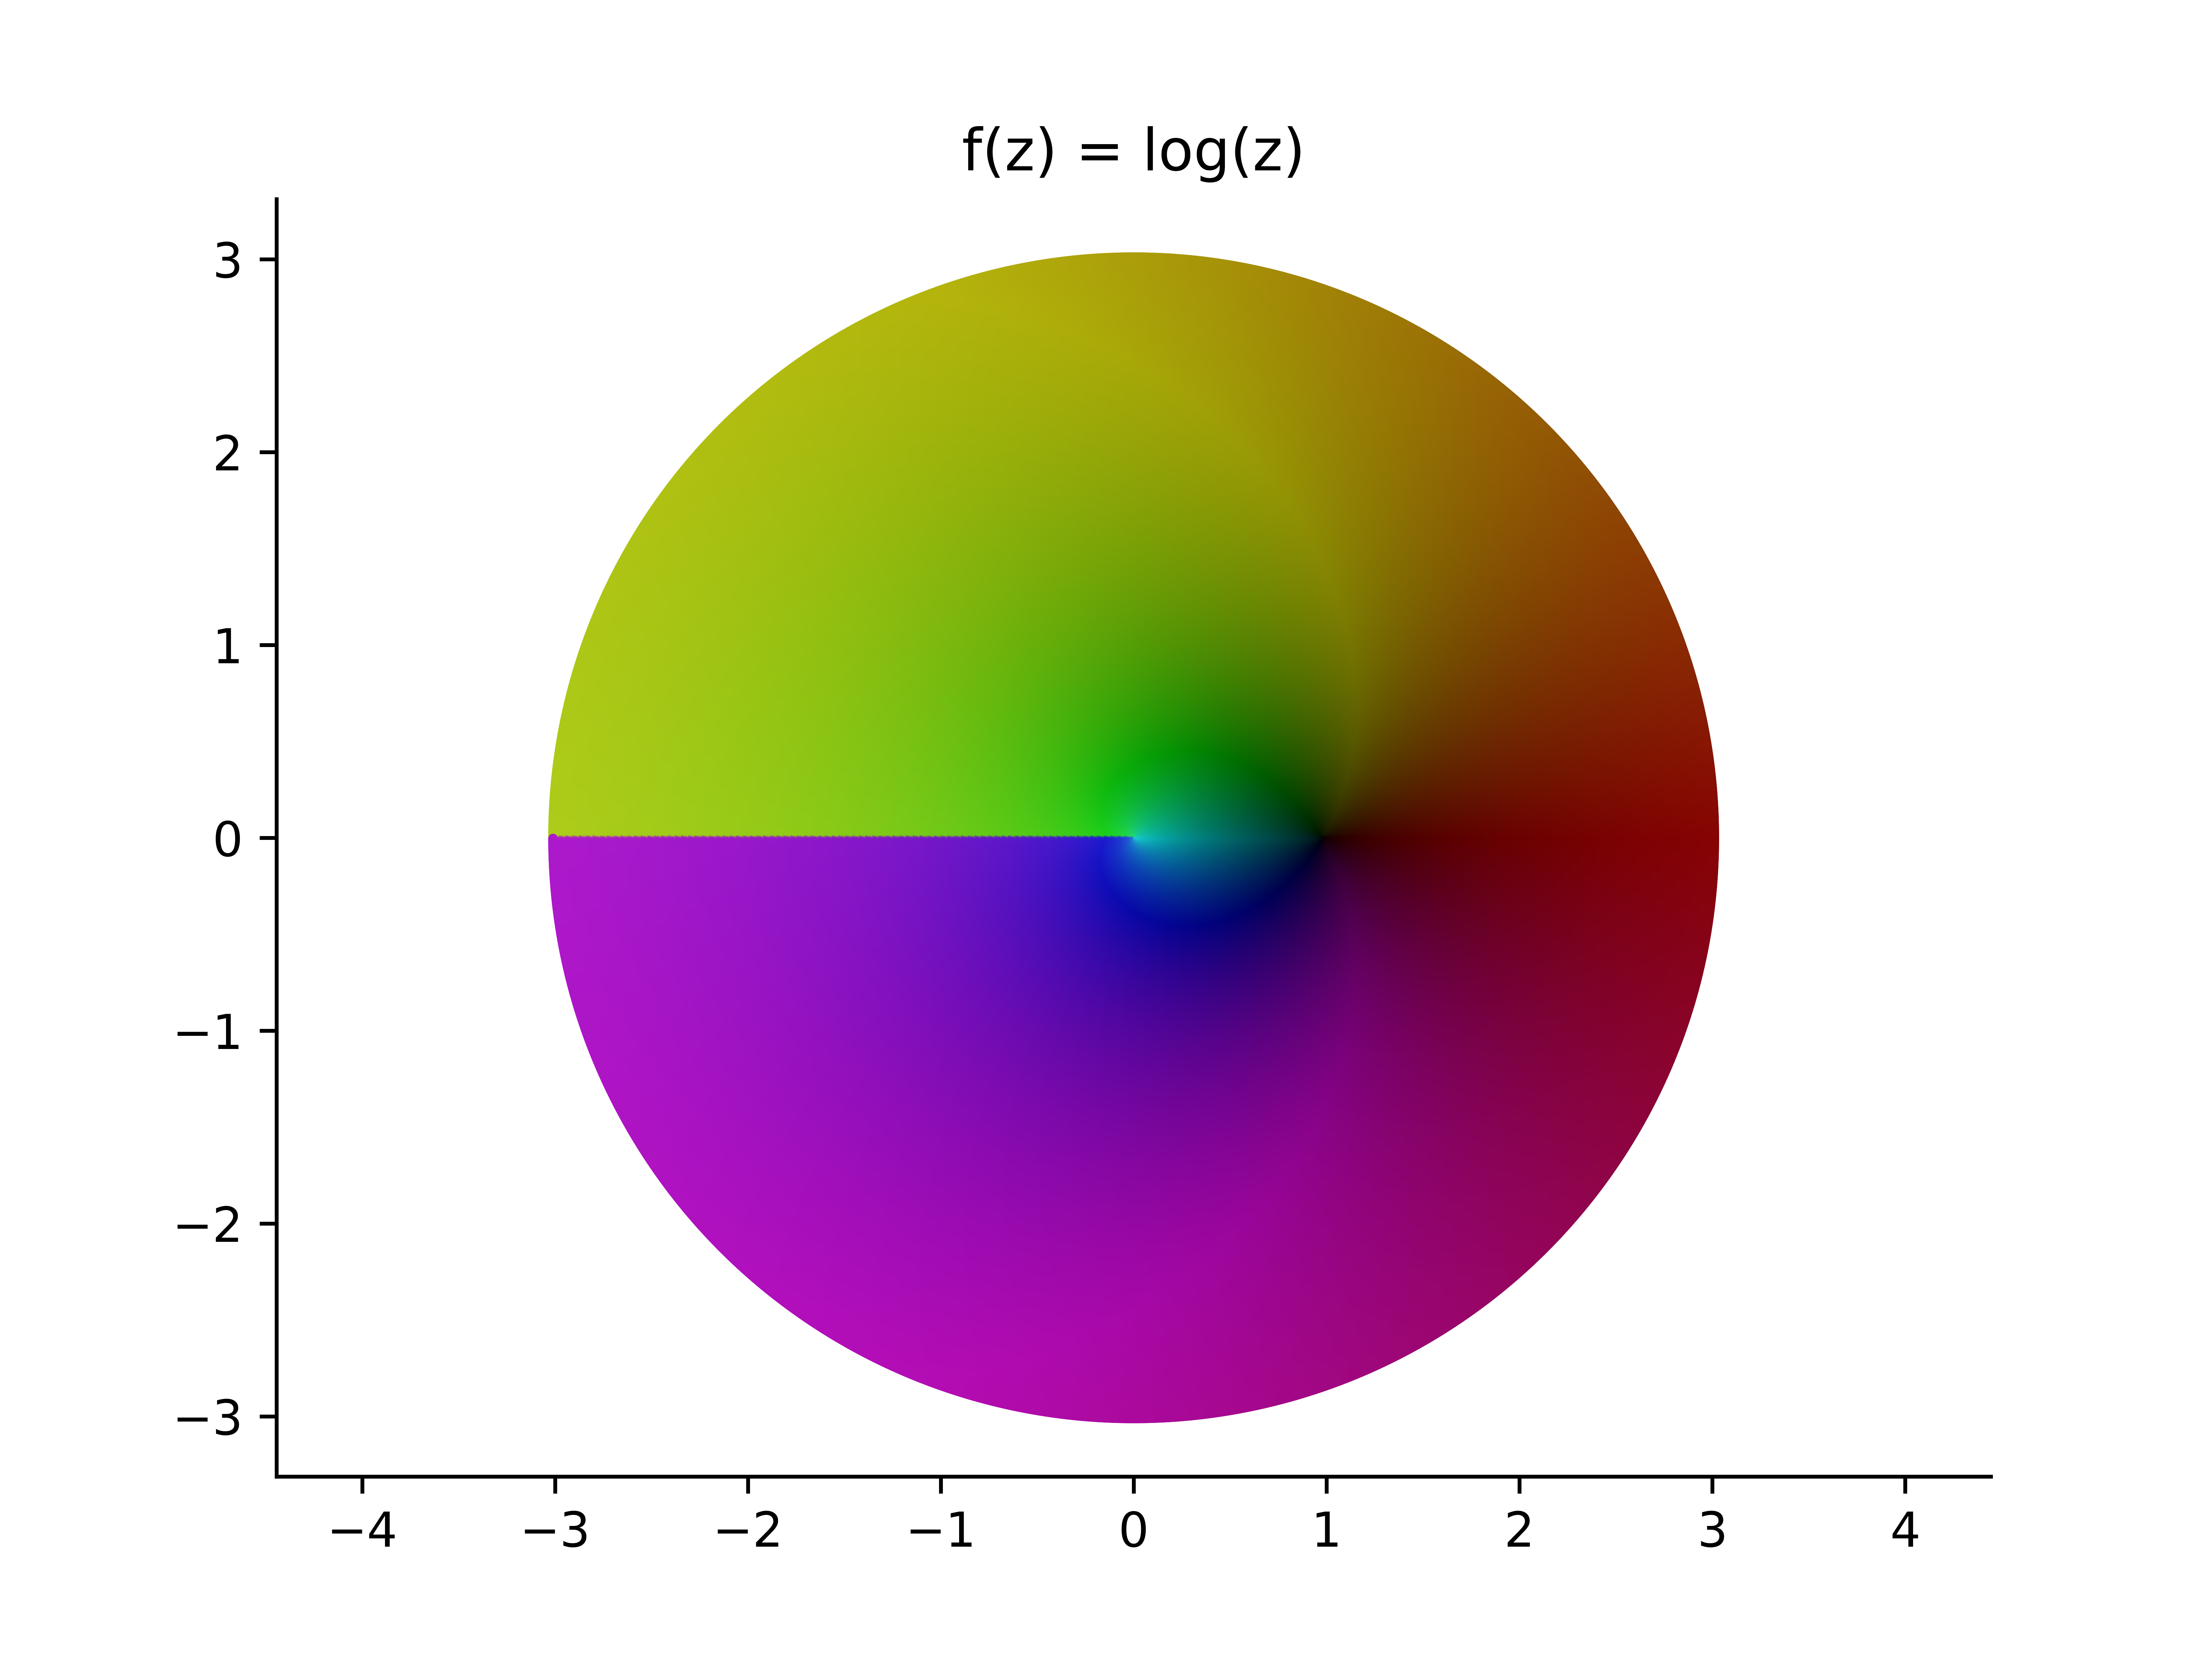
\includegraphics[width=0.7\textwidth]{../Aplicacion/log(z).png}
    \caption{Representación de la función $f(z) = \log(z)$.}
    \label{fig:log(z)}
\end{figure}

Por último, la figura \ref{fig:z^8-2z^7+2z^6-4z^5+2z^4-2z^3-5z^2+4z-4} es la representación de la función $f(z) = z^8-2z^7+2z^6-4z^5+2z^4-2z^3-5z^2+4z-4$ mediante la técnica del coloreado. Las raíces de $f$ vienen representadas por los $6$ puntos negros en el dibujo. Sin embargo, este polinomio tiene $8$ raíces de las cuales $2$ son raíces dobles. Las raíces simples ocurren en los puntos $-1$, $2$ y $\frac{(-1 \rpm i \sqrt{7})}{2}$, y las raíces dobles en $\frac{1 \rpm i \sqrt{3}}{2}$.  La región que rodea a las raíces dobles es algo más oscura que la que rodea a las raíces simples, y en las raíces dobles los colores del círculo cromático la envuelven dos veces, mientras que en las raíces simples la envuelven una sola vez. \\

Además, el dibujo también muestra que el polinomio es de grado $8$. Para $z$ de módulo grande, el término de $z^8$ domina a los otros términos, y por consiguiente la parte exterior del dibujo es similar a la representación de la función $z^8$. Esto puede observarse en que los colores del círculo cromático aparecen ocho veces. \\

\begin{figure}[!htbp]
    \centering
    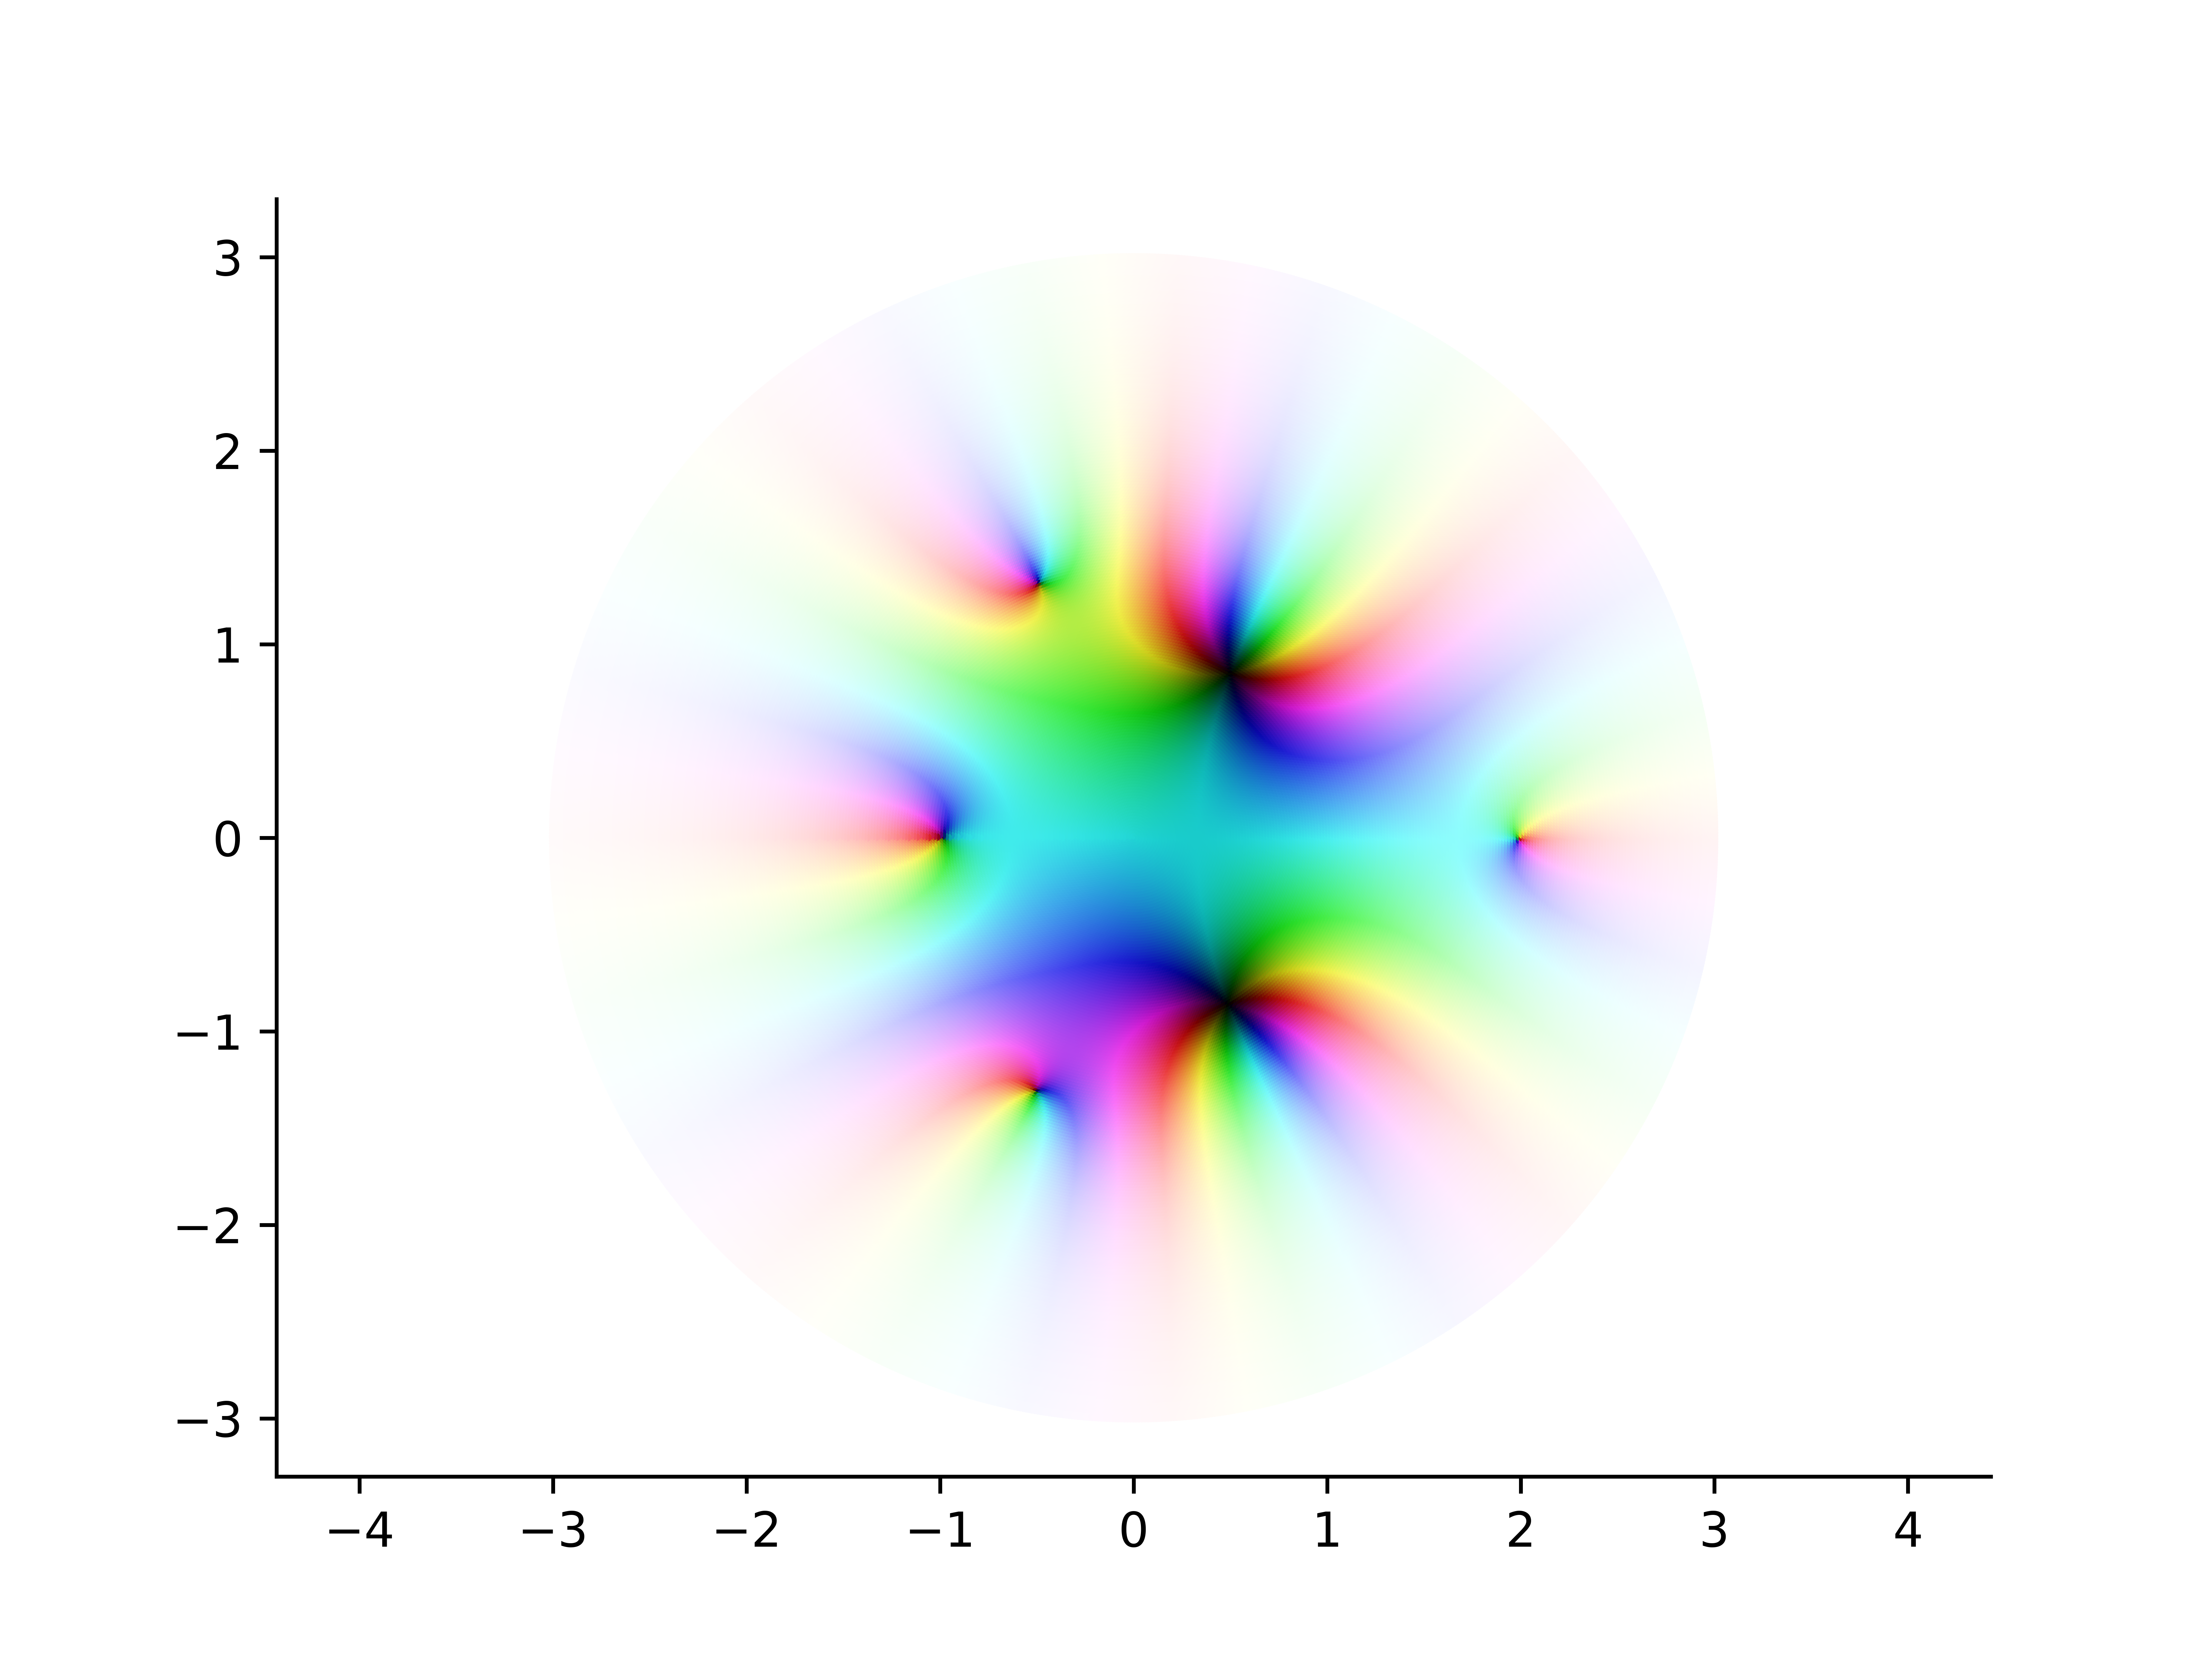
\includegraphics[width=0.7\textwidth]{../Aplicacion/z^8-2z^7+2z^6-4z^5+2z^4-2z^3-5z^2+4z-4.png}
    \caption{$f(z) = z^8-2z^7+2z^6-4z^5+2z^4-2z^3-5z^2+4z-4$}
    \label{fig:z^8-2z^7+2z^6-4z^5+2z^4-2z^3-5z^2+4z-4}
\end{figure}

Introducimos un modelo de color gracias al cual vamos a poder representar fácilmente funciones complejas siguiendo el esquema de asignación de colores explicado anteriormente. Dicho modelo se conoce como HSV (del inglés, \textit{Hue, Saturation, Value} - Tono, Saturación, Valor). \\

El primero de los atributos, que determina el tono de un color, se puede especificar por el ángulo que ocupa alrededor de un punto. Según va aumentando el ángulo, el color va variando de rojo -para los números reales positivos-, amarillo, verde, cyan, azul, magenta para volver de nuevo al rojo. Así pues el tono asociado a un número complejo está directamente relacionado con su argumento. Por otra parte, la saturación es la intensidad de un tono específico, basándose en la pureza del color: un color muy saturado es vivo e intenso, mientras que un color menos saturado es más descolorido y gris. Por último, el valor indica la cantidad de luz que tiene un color. Cuánto más oscuro sea, menor será su valor y cuánto más claro, mayor. De este modo, la saturación y el valor asociadas a un número complejo están relacionados con el módulo del mismo. \\

\begin{figure}[!htbp]
    \begin{minipage}[h]{\textwidth}
        \centering
        \parbox[c][1cm]{\textwidth}{\centering \textbf{Tono}: \\}
        \begin{tikzpicture}[x=1mm,y=1mm]
            \foreach \x in {0,0.0111,...,1}{
                \definecolor{colorhsb}{hsb}{\x, 1, 1}
                \draw[fill=colorhsb, draw=none] (\x*100,1) rectangle +(1mm,7mm);
            }
            \node[below] at (0,1){$0º$};
            \node[below] at (100,1){$360º$};
        \end{tikzpicture}
        \label{fig:hue}
    \end{minipage}
    \begin{minipage}[h]{\textwidth}
        \centering
        \parbox[c][1cm]{\textwidth}{}{\centering \textbf{Saturación}: \\}
        \begin{tikzpicture}[x=1mm,y=1mm]
            \foreach \x in {0,0.0111,...,1}{
                \definecolor{colorhsb}{hsb}{1, \x, 1}
                \draw[fill=colorhsb, draw=none] (\x*100,1) rectangle +(1mm,7mm);
            }
            \node[below] at (0,1){$0º$};
            \node[below] at (100,1){$100º$};
        \end{tikzpicture}
        \label{fig:saturation}
    \end{minipage}
    \begin{minipage}[h]{\textwidth}
        \centering
        \parbox[c][1cm]{\textwidth}{\centering \textbf{Valor}: \\}
        \begin{tikzpicture}[x=1mm,y=1mm]
            \foreach \x in {0,0.0111,...,1}{
                \definecolor{colorhsb}{hsb}{1, 1, \x}
                \draw[fill=colorhsb, draw=none] (\x*100,1) rectangle +(1mm,7mm);
            }
            \node[below] at (0,1){$0º$};
            \node[below] at (100,1){$100º$};
        \end{tikzpicture}
        \label{fig:value}
    \end{minipage}
    \caption{Modelo de color HSV}
    \label{fig:hsv}
\end{figure}

Los colores en Python se pueden dibujar mediante tuplas RGB de valores comprendidos entre el cero y el uno, esto es, $color \, rgb = (r, g, b)$, con $0 \leq r, g, b \leq 1$. Cada uno de estos números se corresponde con uno de los tres colores primarios: rojo (\textit{red}), verde (\textit{green}) y azul (\textit{blue}). Estos colores se representan como: $rojo = (1, 0, 0)$, $verde = (0, 1, 0)$ y $azul = (0, 0, 1)$. Además, el blanco y el negro suponen todos estos valores a cero o a uno ($blanco = (1, 1, 1)$ y $negro = (0, 0, 0)$). \\

Ahora bien, Python también admite una representación de colores por medio de tuplas HSV con valores entre el cero y el uno, es decir, $color \, hsv = (h, s, v)$, con $0 \leq h, s, v \leq 1$. Así que podremos asociar a cada número complejo una terna en el modelo de colores HSV, cuidándonos de que los valores estén dentro del rango adecuado. Además, gracias a una función de Python podemos transformar directamente un color del modelo HSV en RGB. \\

De esta manera podremos representar cualquier color en Python como combinación de su tono, saturación y brillo, que dependen a su vez del módulo y el argumento del número complejo. \\

\section{Representación de funciones. Problema de Dirichlet}

A lo largo del trabajo nos vamos a centrar en el comportamiento de funciones en el borde del disco unidad. Por ello, la representación de funciones se realiza en discos centrados en $0$ de radio arbitrario, siendo $1$ el valor por defecto. La propia forma del dominio sugiere tomar un mallado circular y evaluar la función en cada punto. \\

La aplicación que se ha desarrollado tiene tres funcionalidades diferentes. En primer lugar, permite representar funciones complejas en un disco de radio determinado, como ya se ha mostrado en las figuras de la sección anterior, cuyas representaciones han sido obtenidos al ejecutar el programa realizado. \\

Por otra parte, también se puede resolver el problema de Dirichlet para el disco haciendo uso de la integral de Poisson. Dada una función $f$ definida en el borde del disco, la solución dada por la integral de Poisson definirá una función armónica en el disco abierto. Además, si $f$ es una función continua, la solución será también una función continua en el disco cerrado, que coincidirá con $f$ en el borde del disco. \\

La función $f$ que recibe el programa parametriza el borde del disco en función del argumento. Así pues, para poder definir funciones con mayor facilidad, su dominio de definición es $[-\pi, \pi]$ de manera que $\theta \in [-\pi, \pi]$ se corresponde con el punto $z = e^{i \theta} = \cos(\theta) + i \sen(\theta) \in \partial \disk$. \\

Podemos utilizar la representación de funciones que se ha desarrollado para comprobar que la integral de Poisson se comporta como se espera cuando la parametrización dada se corresponde, en el borde, con la función que se va a dibujar. A continuación se pueden observar algunos ejemplos. \\

La figura \ref{fig:comp_e^z} se corresponde con la extensión al disco de la función $f : [-\pi, \pi] \to \complex, t \to e^{10 \cos(t)+10i \sen(t)}$. A su vez, esta función parametriza el borde del disco de tal manera que cada punto $t \in [-\pi, \pi]$ se corresponde con un punto $z = e^{i \theta} = \cos(\theta) + i \sen(\theta) \in \partial \disk$. Deshaciendo este cambio, obtenemos que la función $f$ se puede escribir como $f: \partial \disk \to \complex, z \mapsto e^{10z}$. Volviendo a la figura \ref{fig:e^z} podemos comprobar que se trata de la misma representación. \\

\begin{figure}[!htbp]
    \centering
    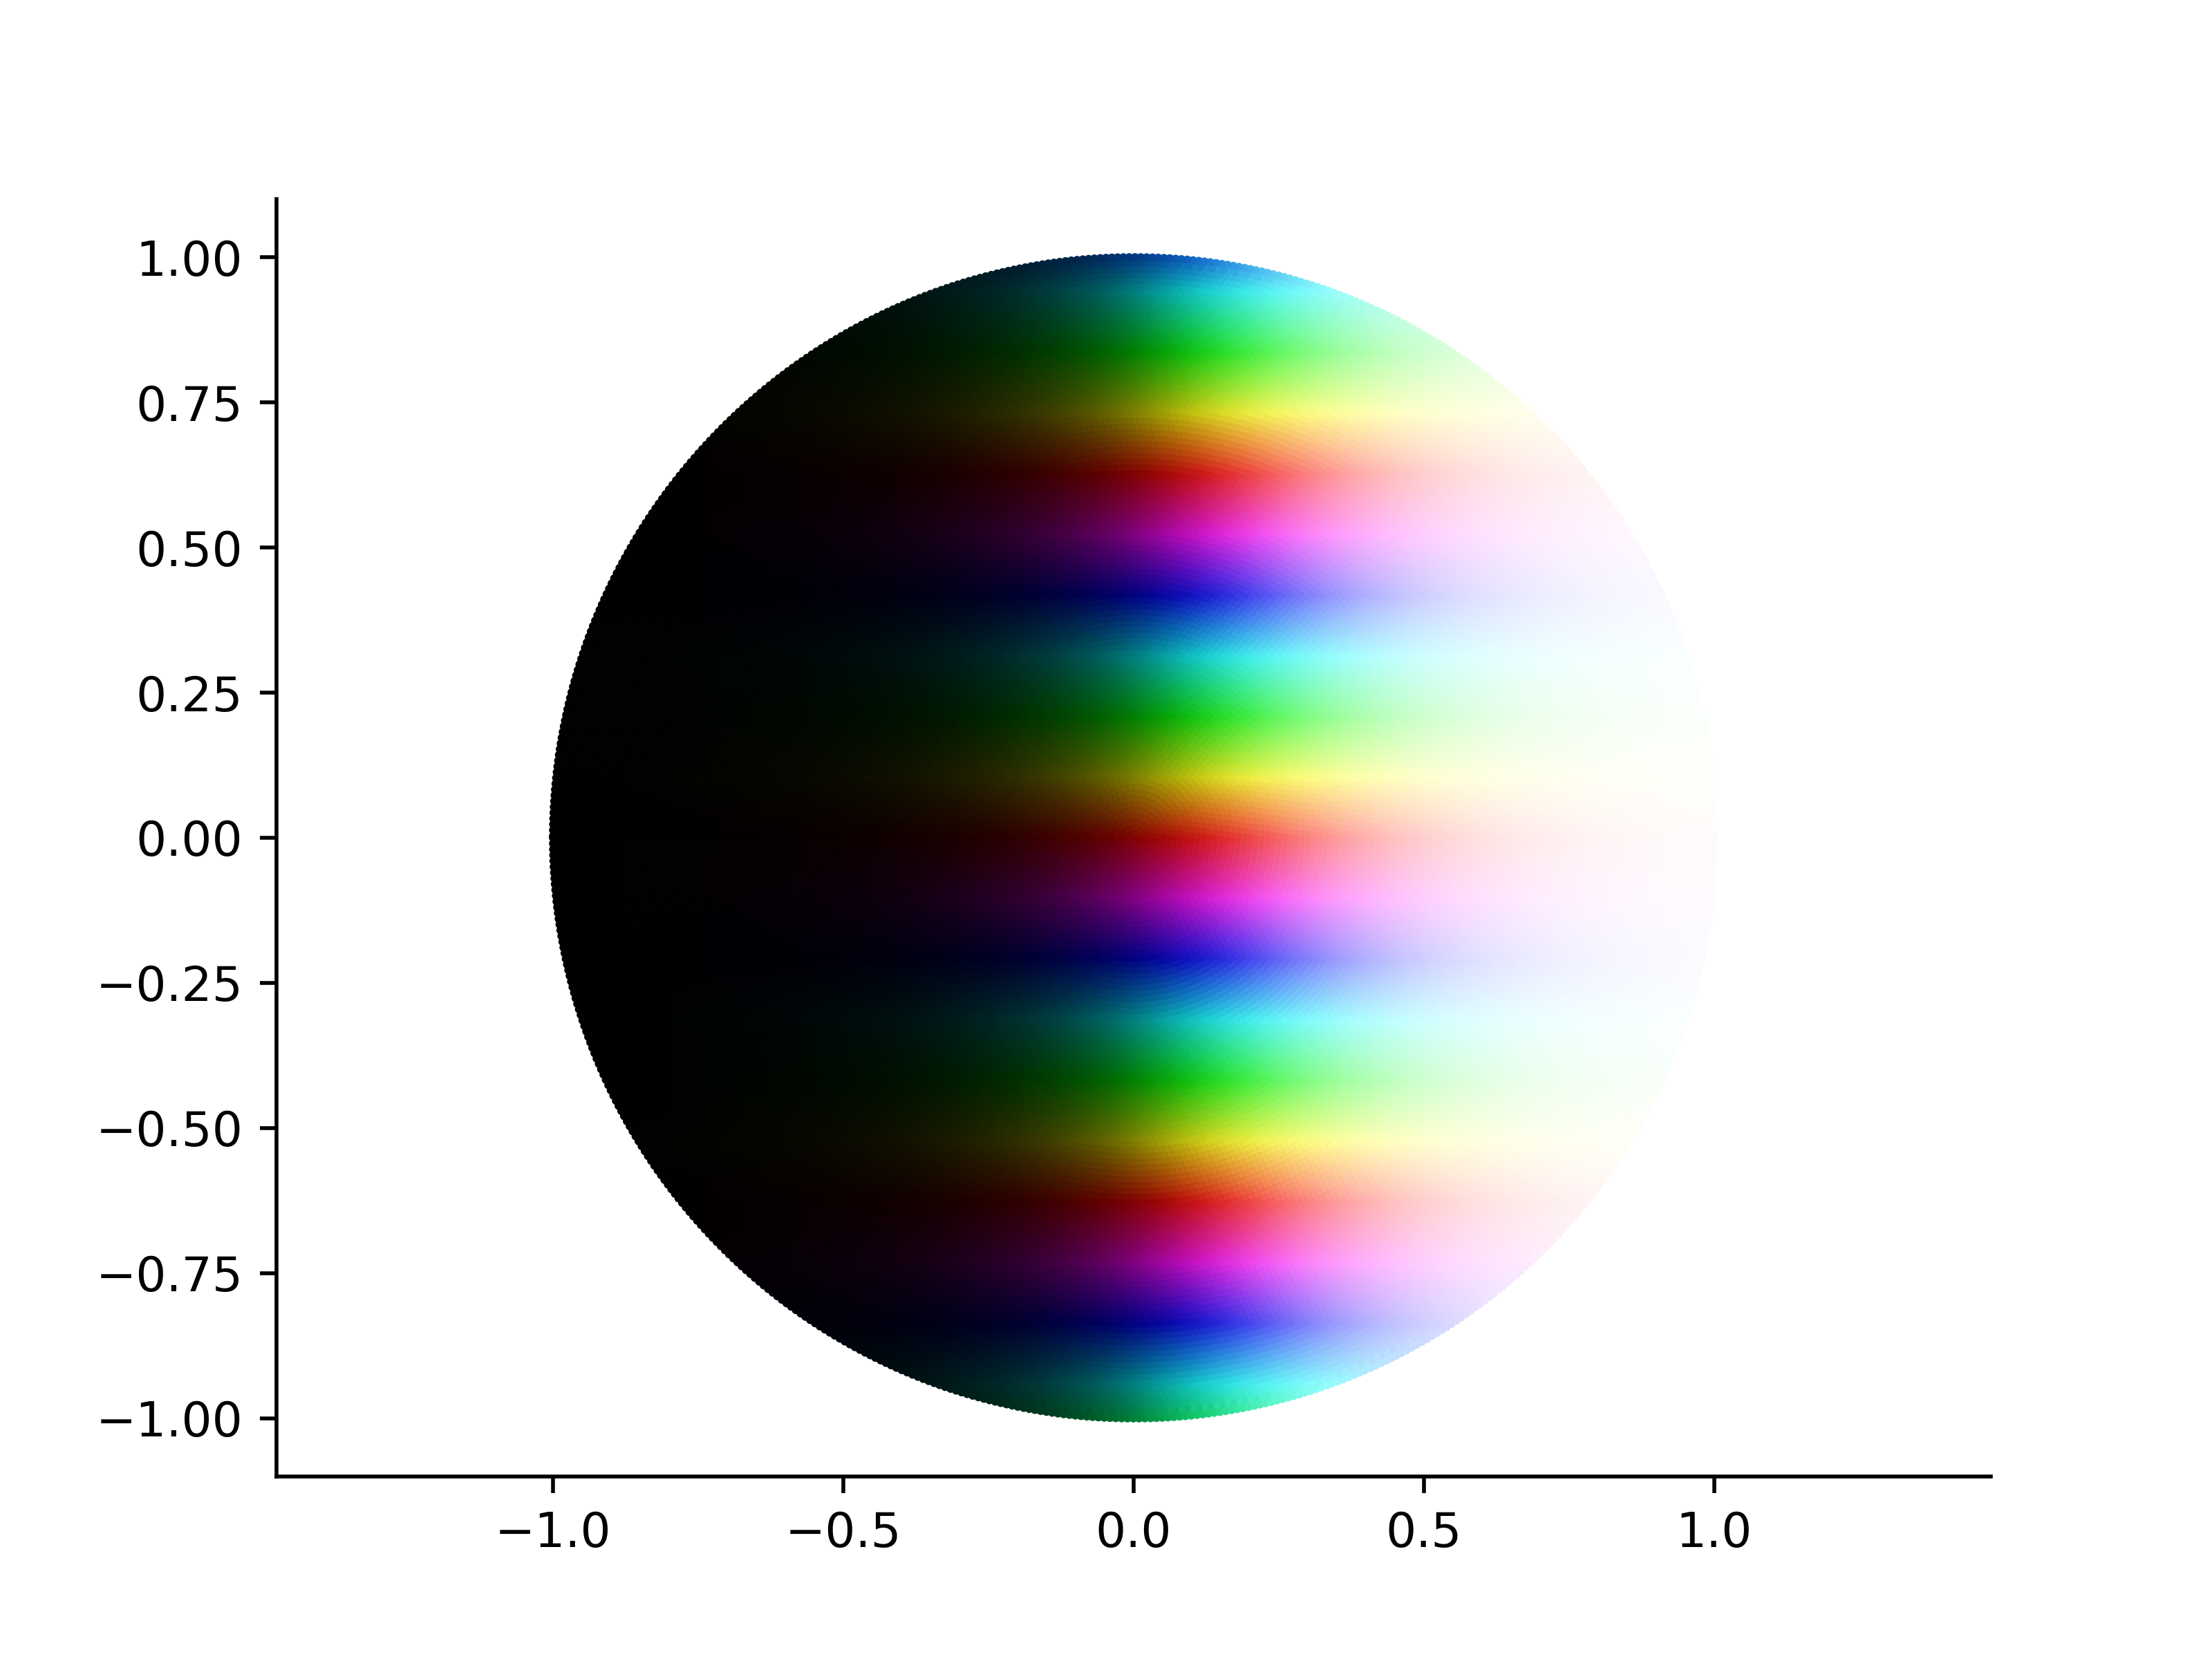
\includegraphics[width=0.7\textwidth]{../Aplicacion/e^(10cos(t)+10isen(t)).png}
    \caption{Extensión al disco de la función $f(t) = e^{10 \cos(t)+10i \sen(t)}$.}
    \label{fig:comp_e^z}
\end{figure}

La figura \ref{fig:comp_z} representa la extensión al disco de la función $f: [-\pi, \pi] \to \complex, t \to 10(\cos(t)+10i \sen(t))$. Deshaciendo este cambio como en el ejemplo anterior, tenemos que la función $f$ se puede escribir de la siguiente manera $f: \partial \disk \to \complex, z \mapsto 10z$. De nuevo, si nos fijamos en la figura \ref{fig:z} podemos observar que coinciden. \\

\begin{figure}[!htbp]
    \centering
    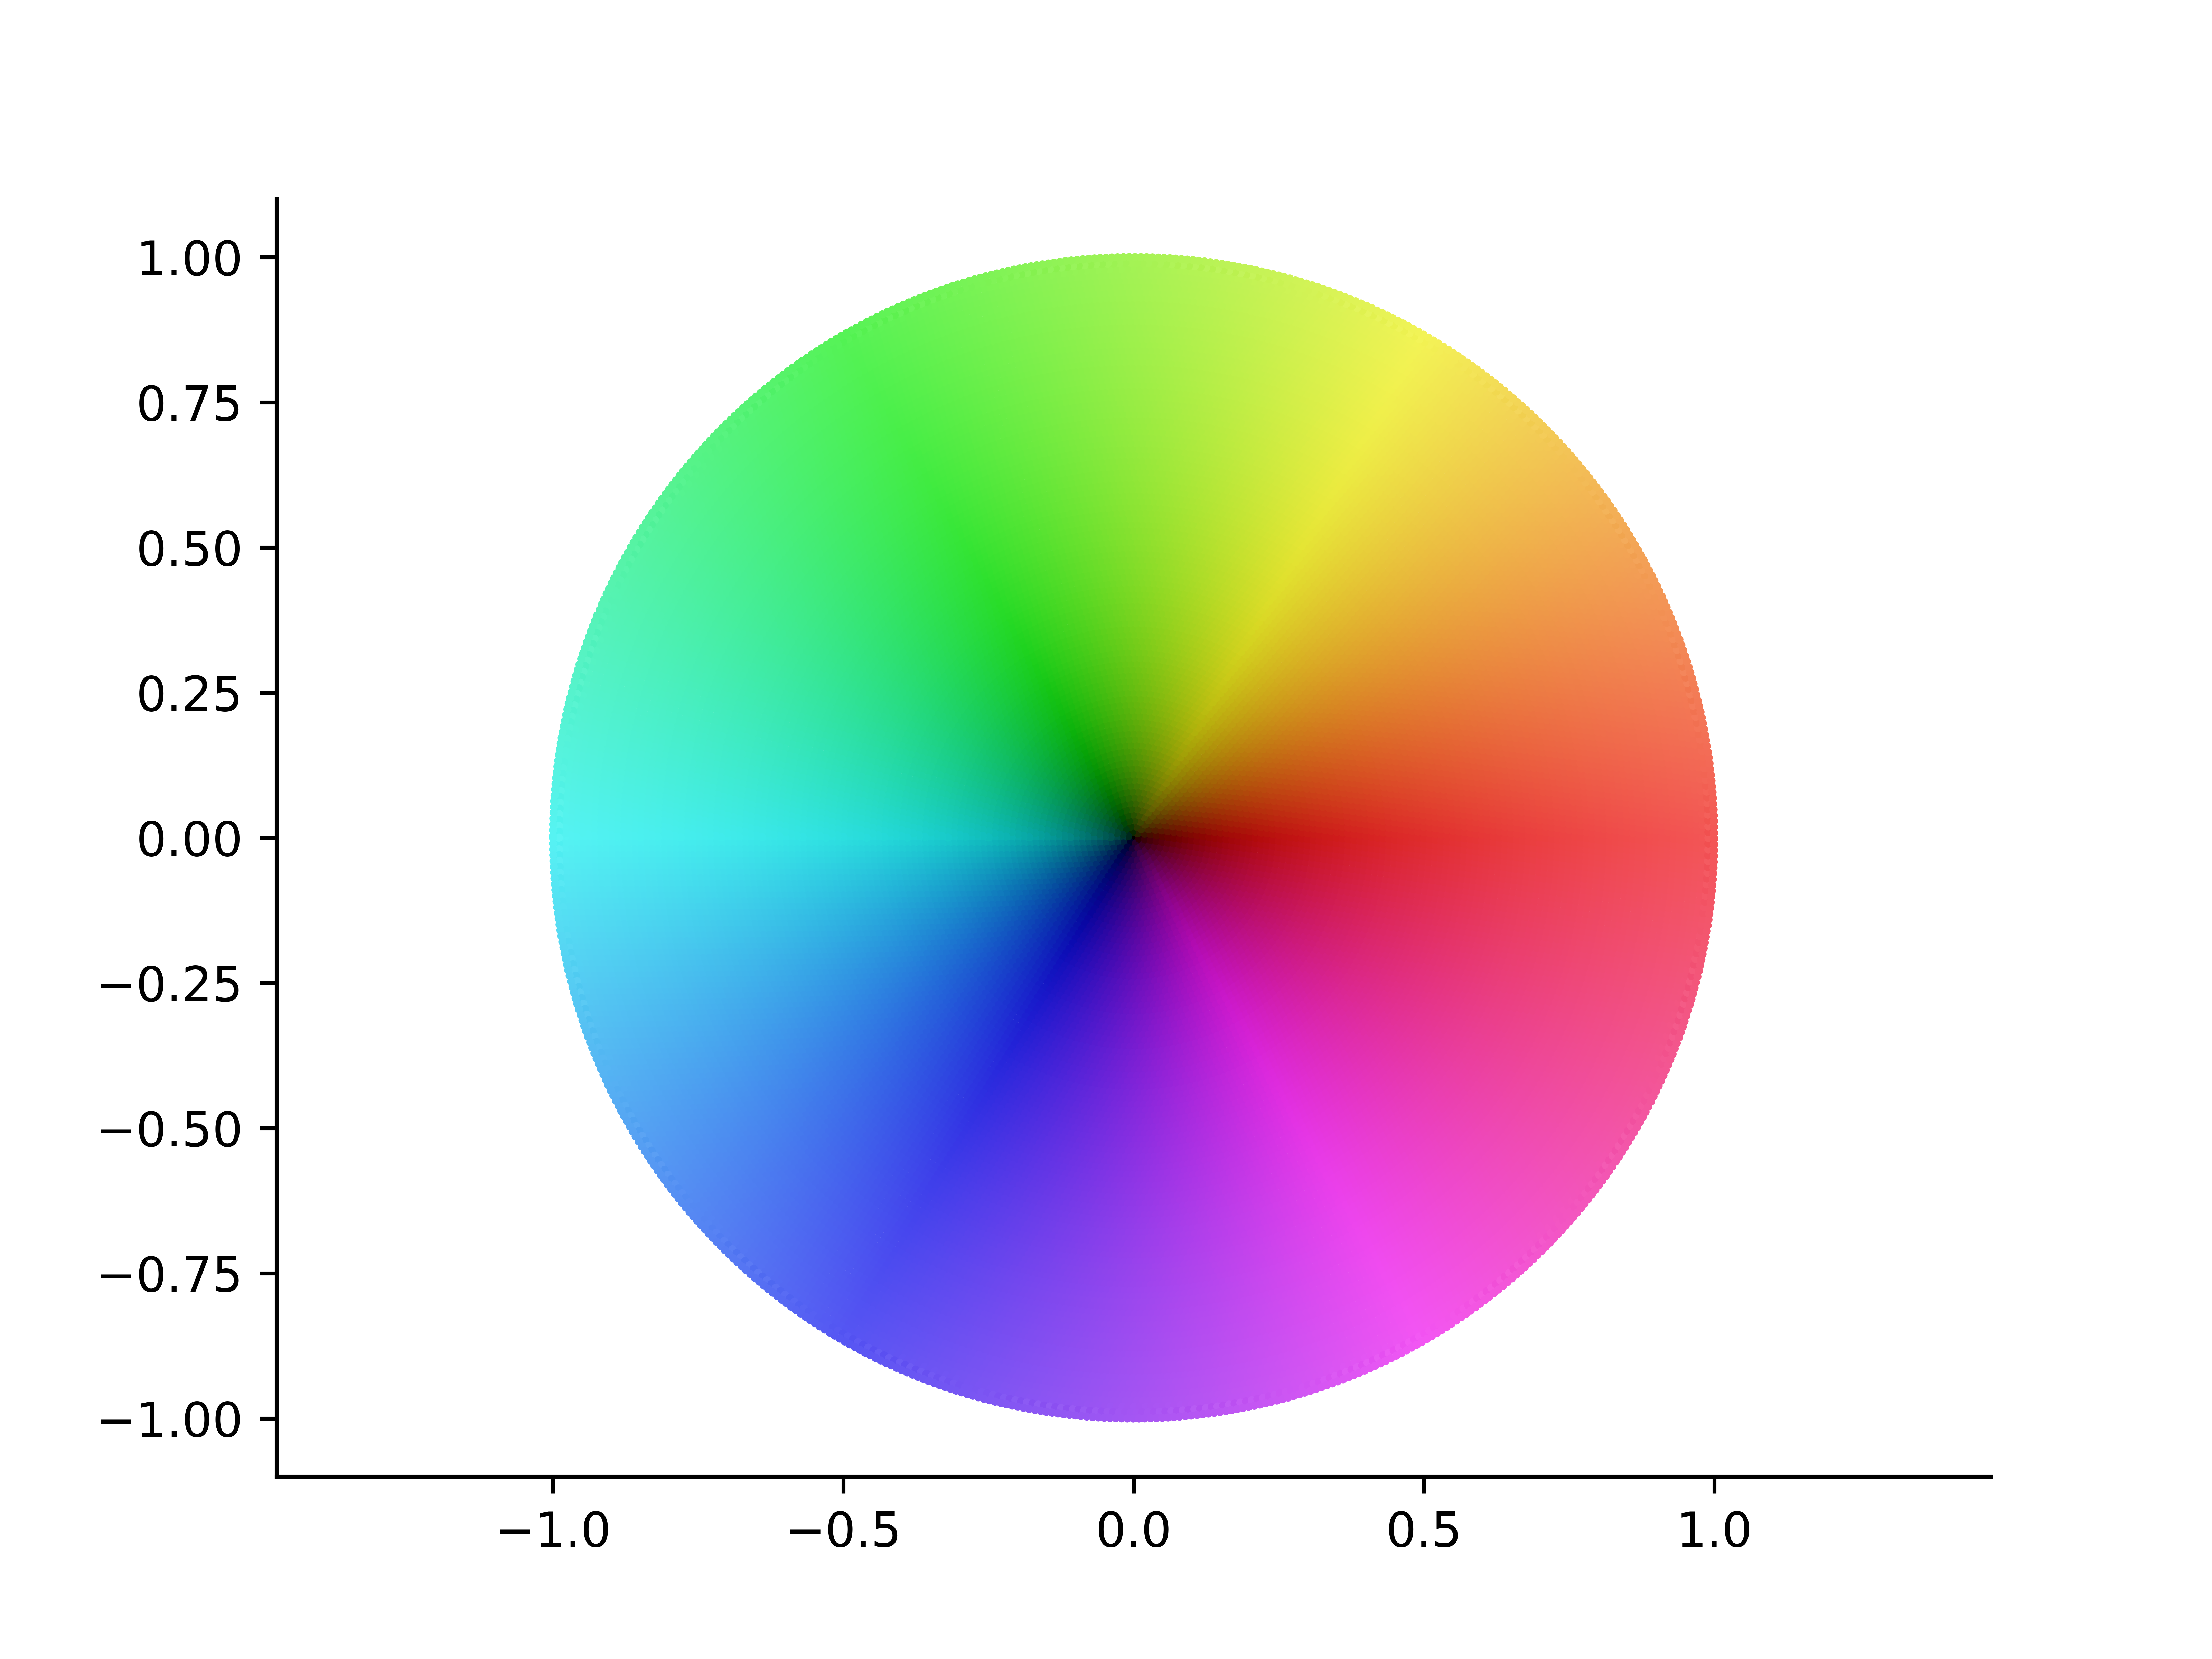
\includegraphics[width=0.7\textwidth]{../Aplicacion/10cos(t)+10isen(t).png}
    \caption{Extensión al disco de la función $f(t) = 10(\cos(t) + i \sen(t))$.}
    \label{fig:comp_z}
\end{figure}

La figura \ref{fig:comp_z^3} muestra la extensión al disco de la función $f: [-\pi, \pi] \to \complex, t \to (5\cos(t)+5i \sen(t))^3$ que se corresponde con  $f: \partial \disk \to \complex, z \mapsto (5z)^3$. Esta representación coincide con la que se observa en la figura \ref{fig:z^3}. \\

\begin{figure}[!htbp]
    \centering
    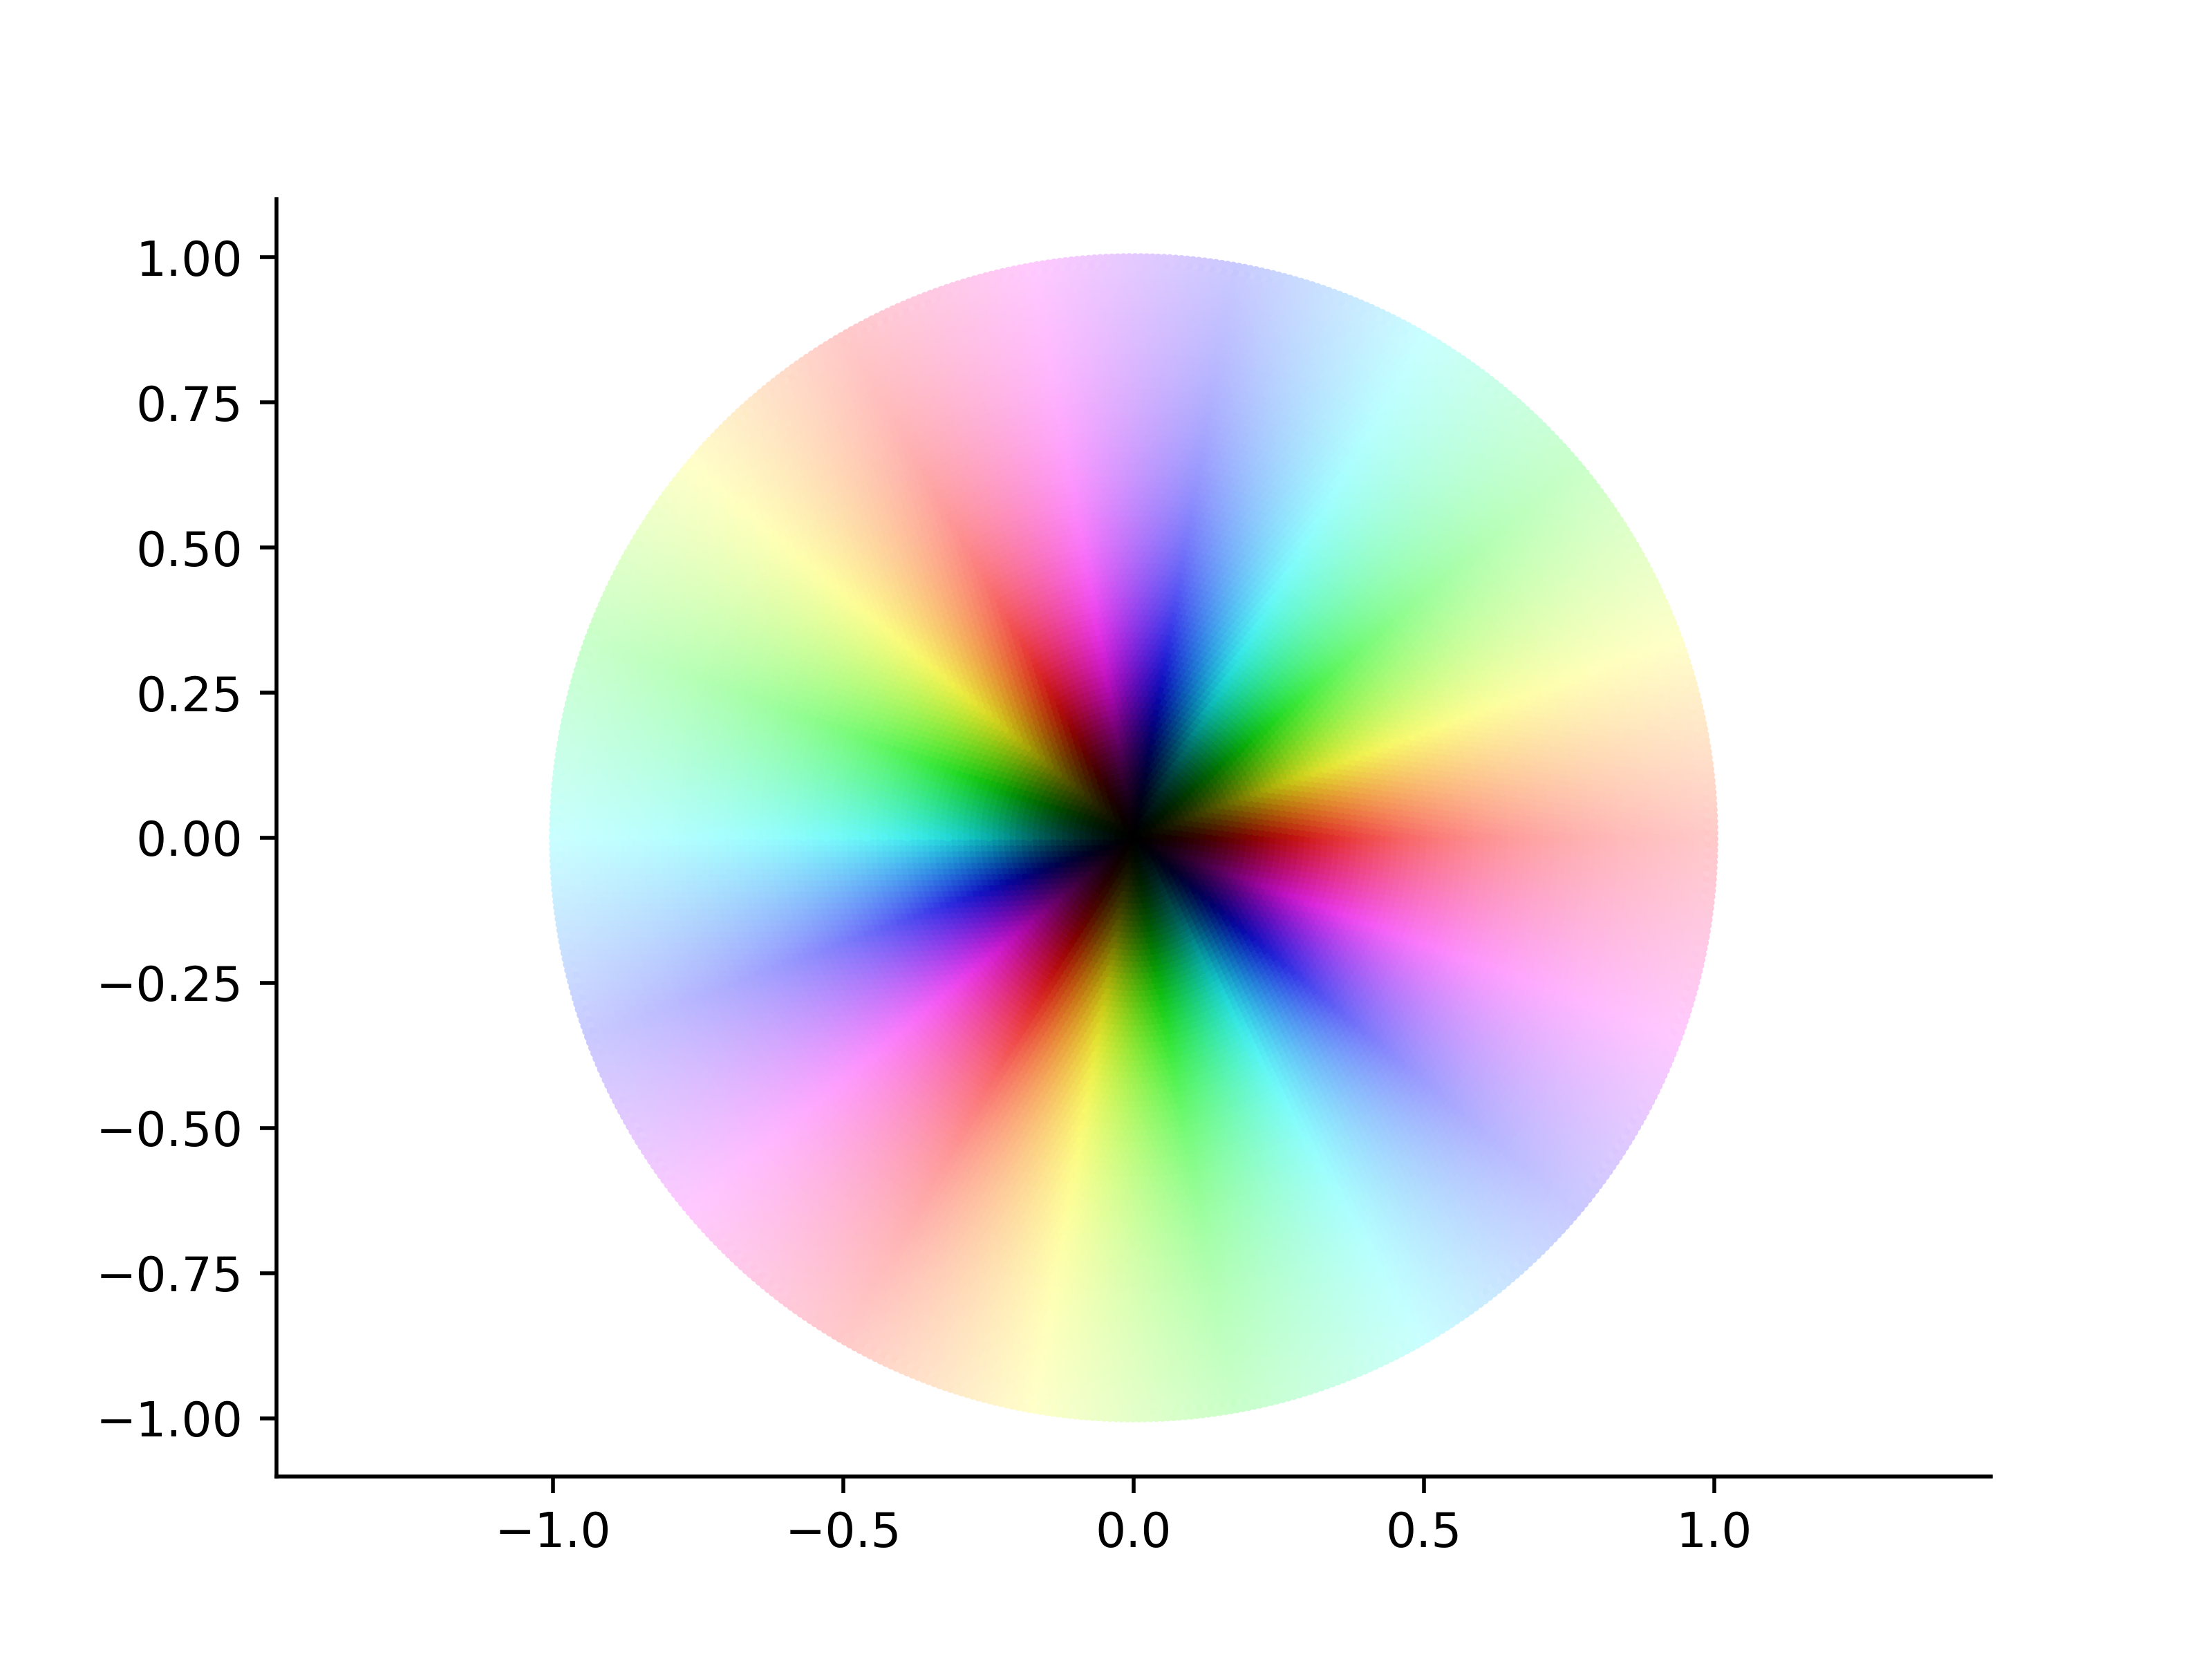
\includegraphics[width=0.7\textwidth]{../Aplicacion/(5cos(t)+5isen(t))^3.png}
    \caption{Extensión al disco de la función $f(t) = (5\cos(t)+ 5i \sen(t))^3$.}
    \label{fig:comp_z^3}
\end{figure}

Por último, la figura \ref{fig:comparacion4} se corresponde con la extensión al disco de la función $f: [-\pi, \pi] \to \complex, t \to \cos^2(t)-\sen^2(t)$ que también puede escribirse como $f: \partial \disk \to \complex, z \mapsto \Re(z^2)$. \\

\begin{figure}[!htbp]
    \centering
    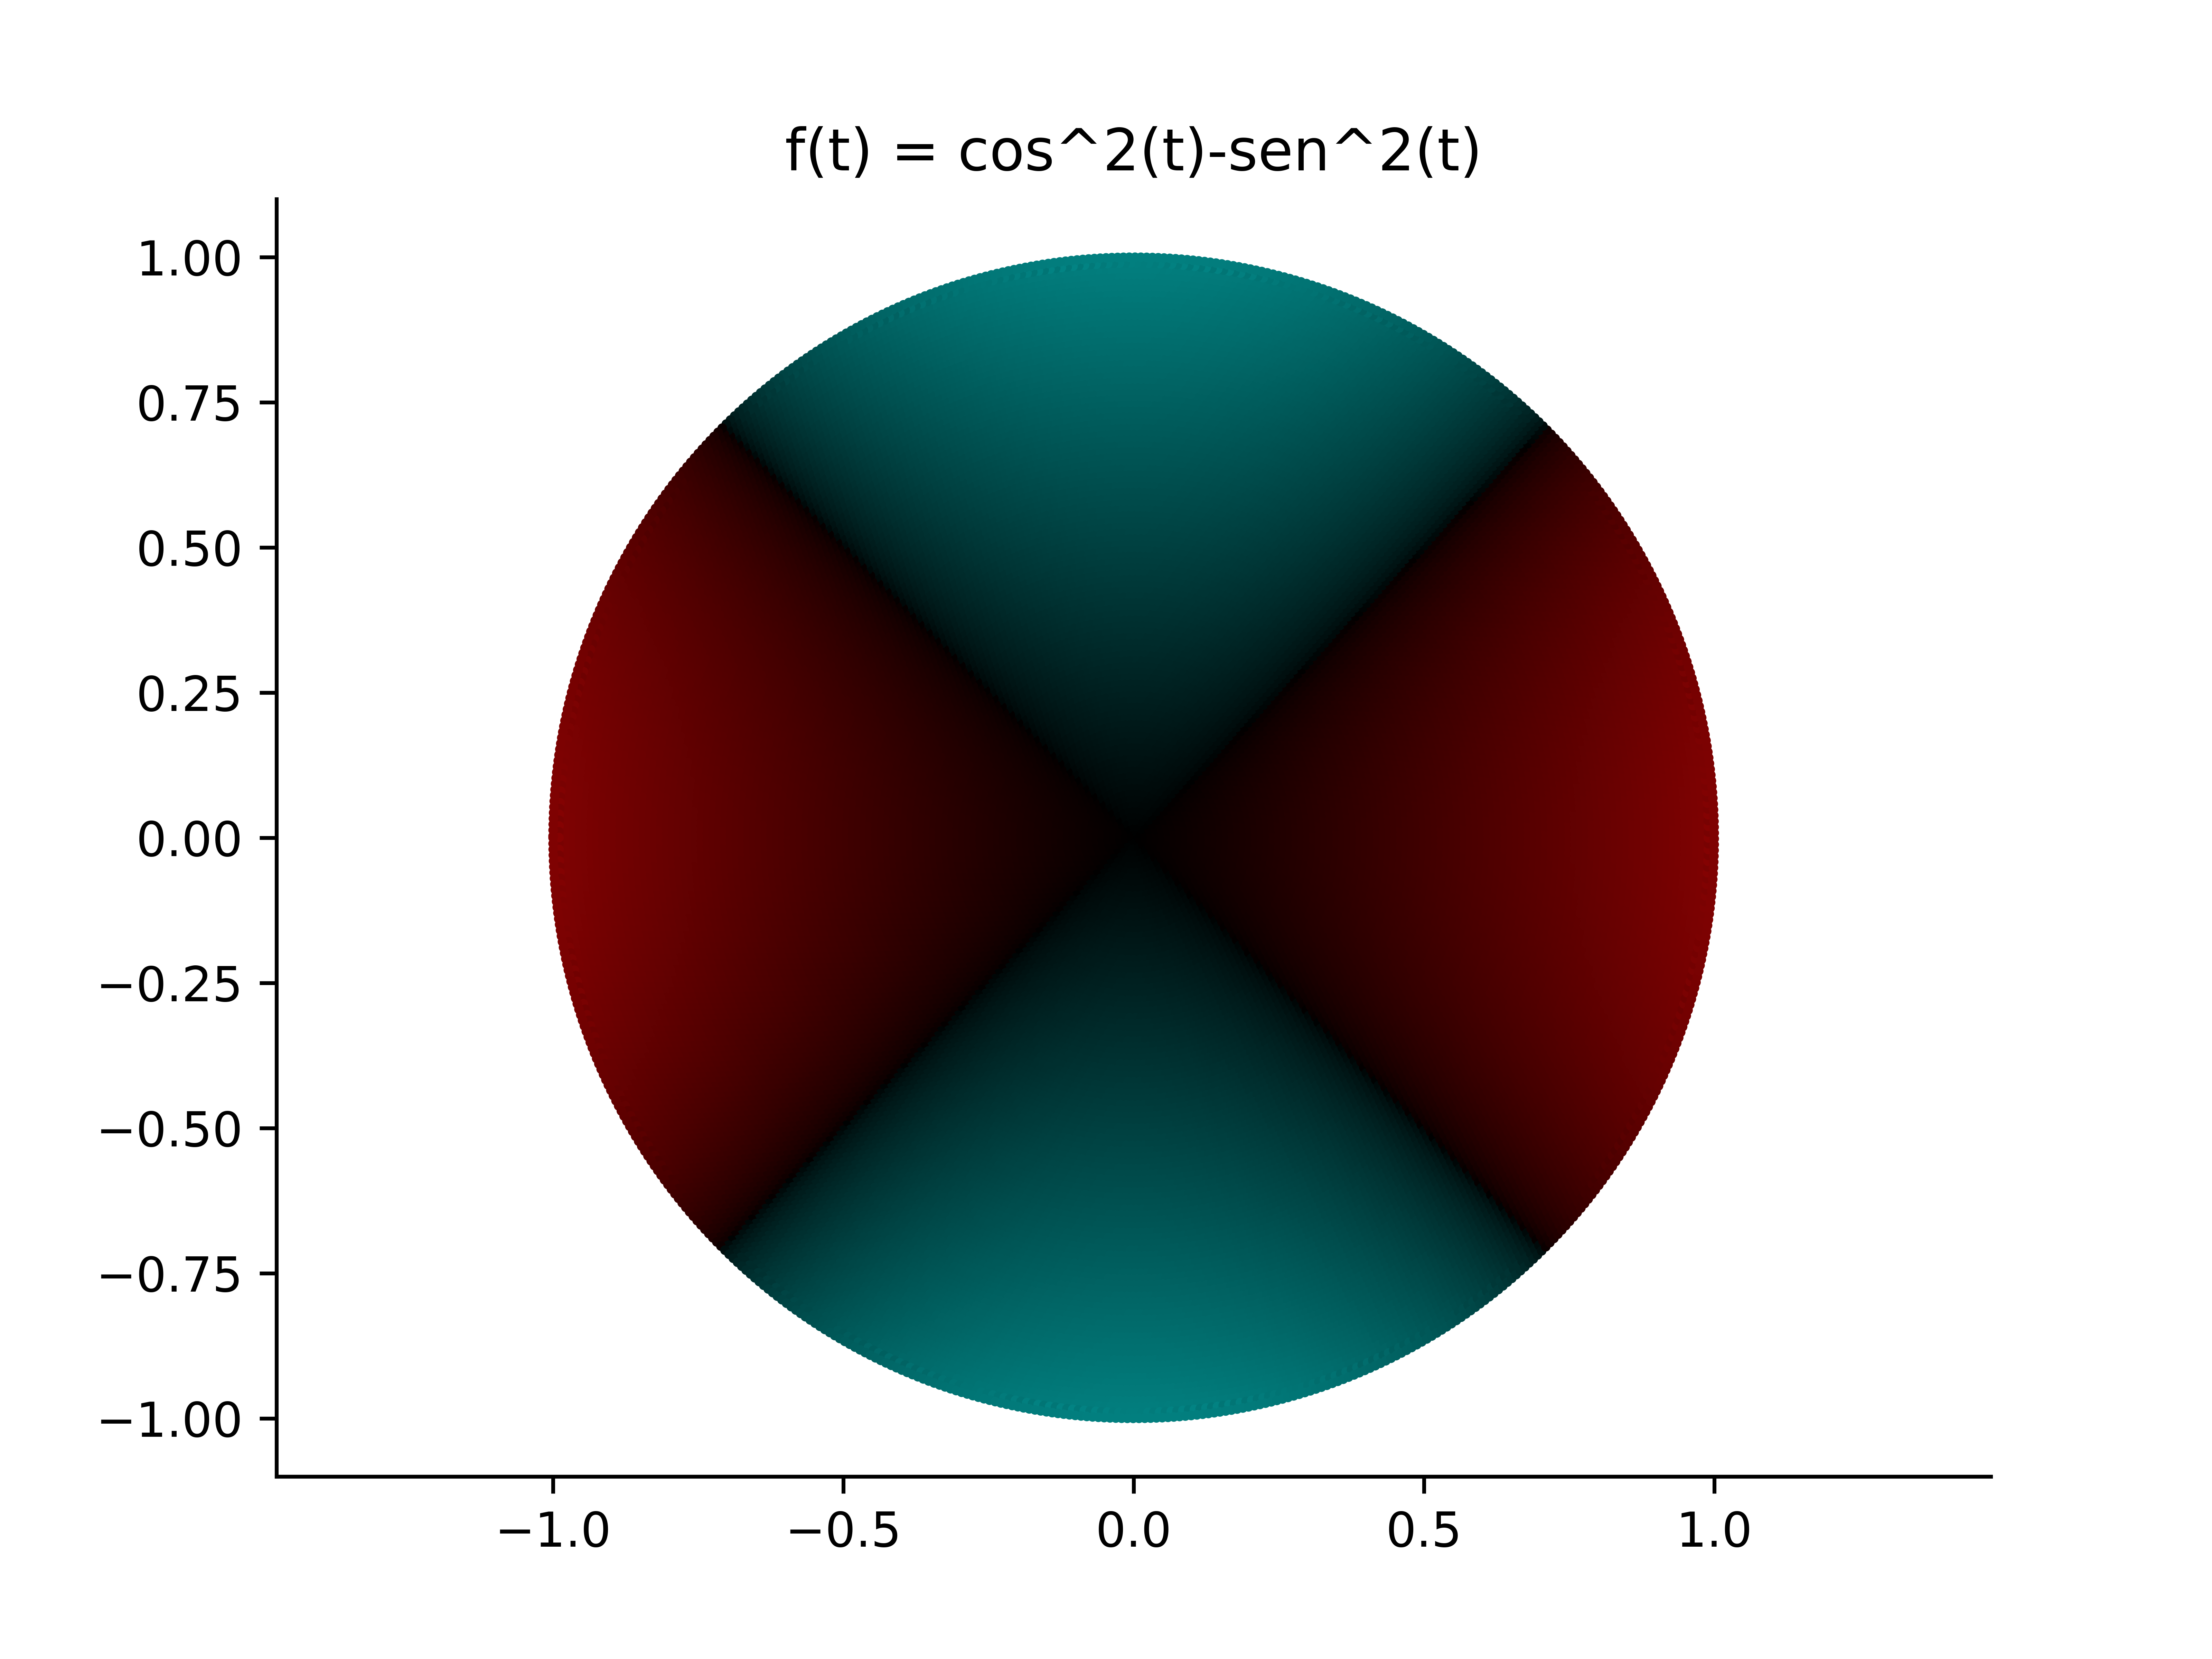
\includegraphics[width=0.7\textwidth]{../Aplicacion/cos^2(t)-sen^2(t).png}
    \caption{Extensión al disco de la función $f(t) = \cos^2(t) - \sen^2(t)$.}
    \label{fig:comparacion4}
\end{figure}

Esta misma comprobación se puede llevar a cabo mediante la última funcionalidad de la aplicación que permite representar la diferencia de funciones. Por lo tanto, si el cálculo de la integral de Poisson fuera perfecto, el dibujo resultante sería negro en su totalidad. Esto se consigue en la mayoría de los ejemplos, con funciones acotadas por valores no muy grandes. \\

Sin embargo, debido a errores numéricos, este cálculo no es totalmente exacto y presenta algunas inexactitudes sobre todo en puntos cercanos al borde del disco o cuyo módulo, a través de la función, es grande. Podemos ver esto reflejado en la figura \ref{fig:diferencia} que muestra la diferencia entre las figuras \ref{fig:comp_e^z} y \ref{fig:e^z}. \\

\begin{figure}[!htbp]
    \centering
    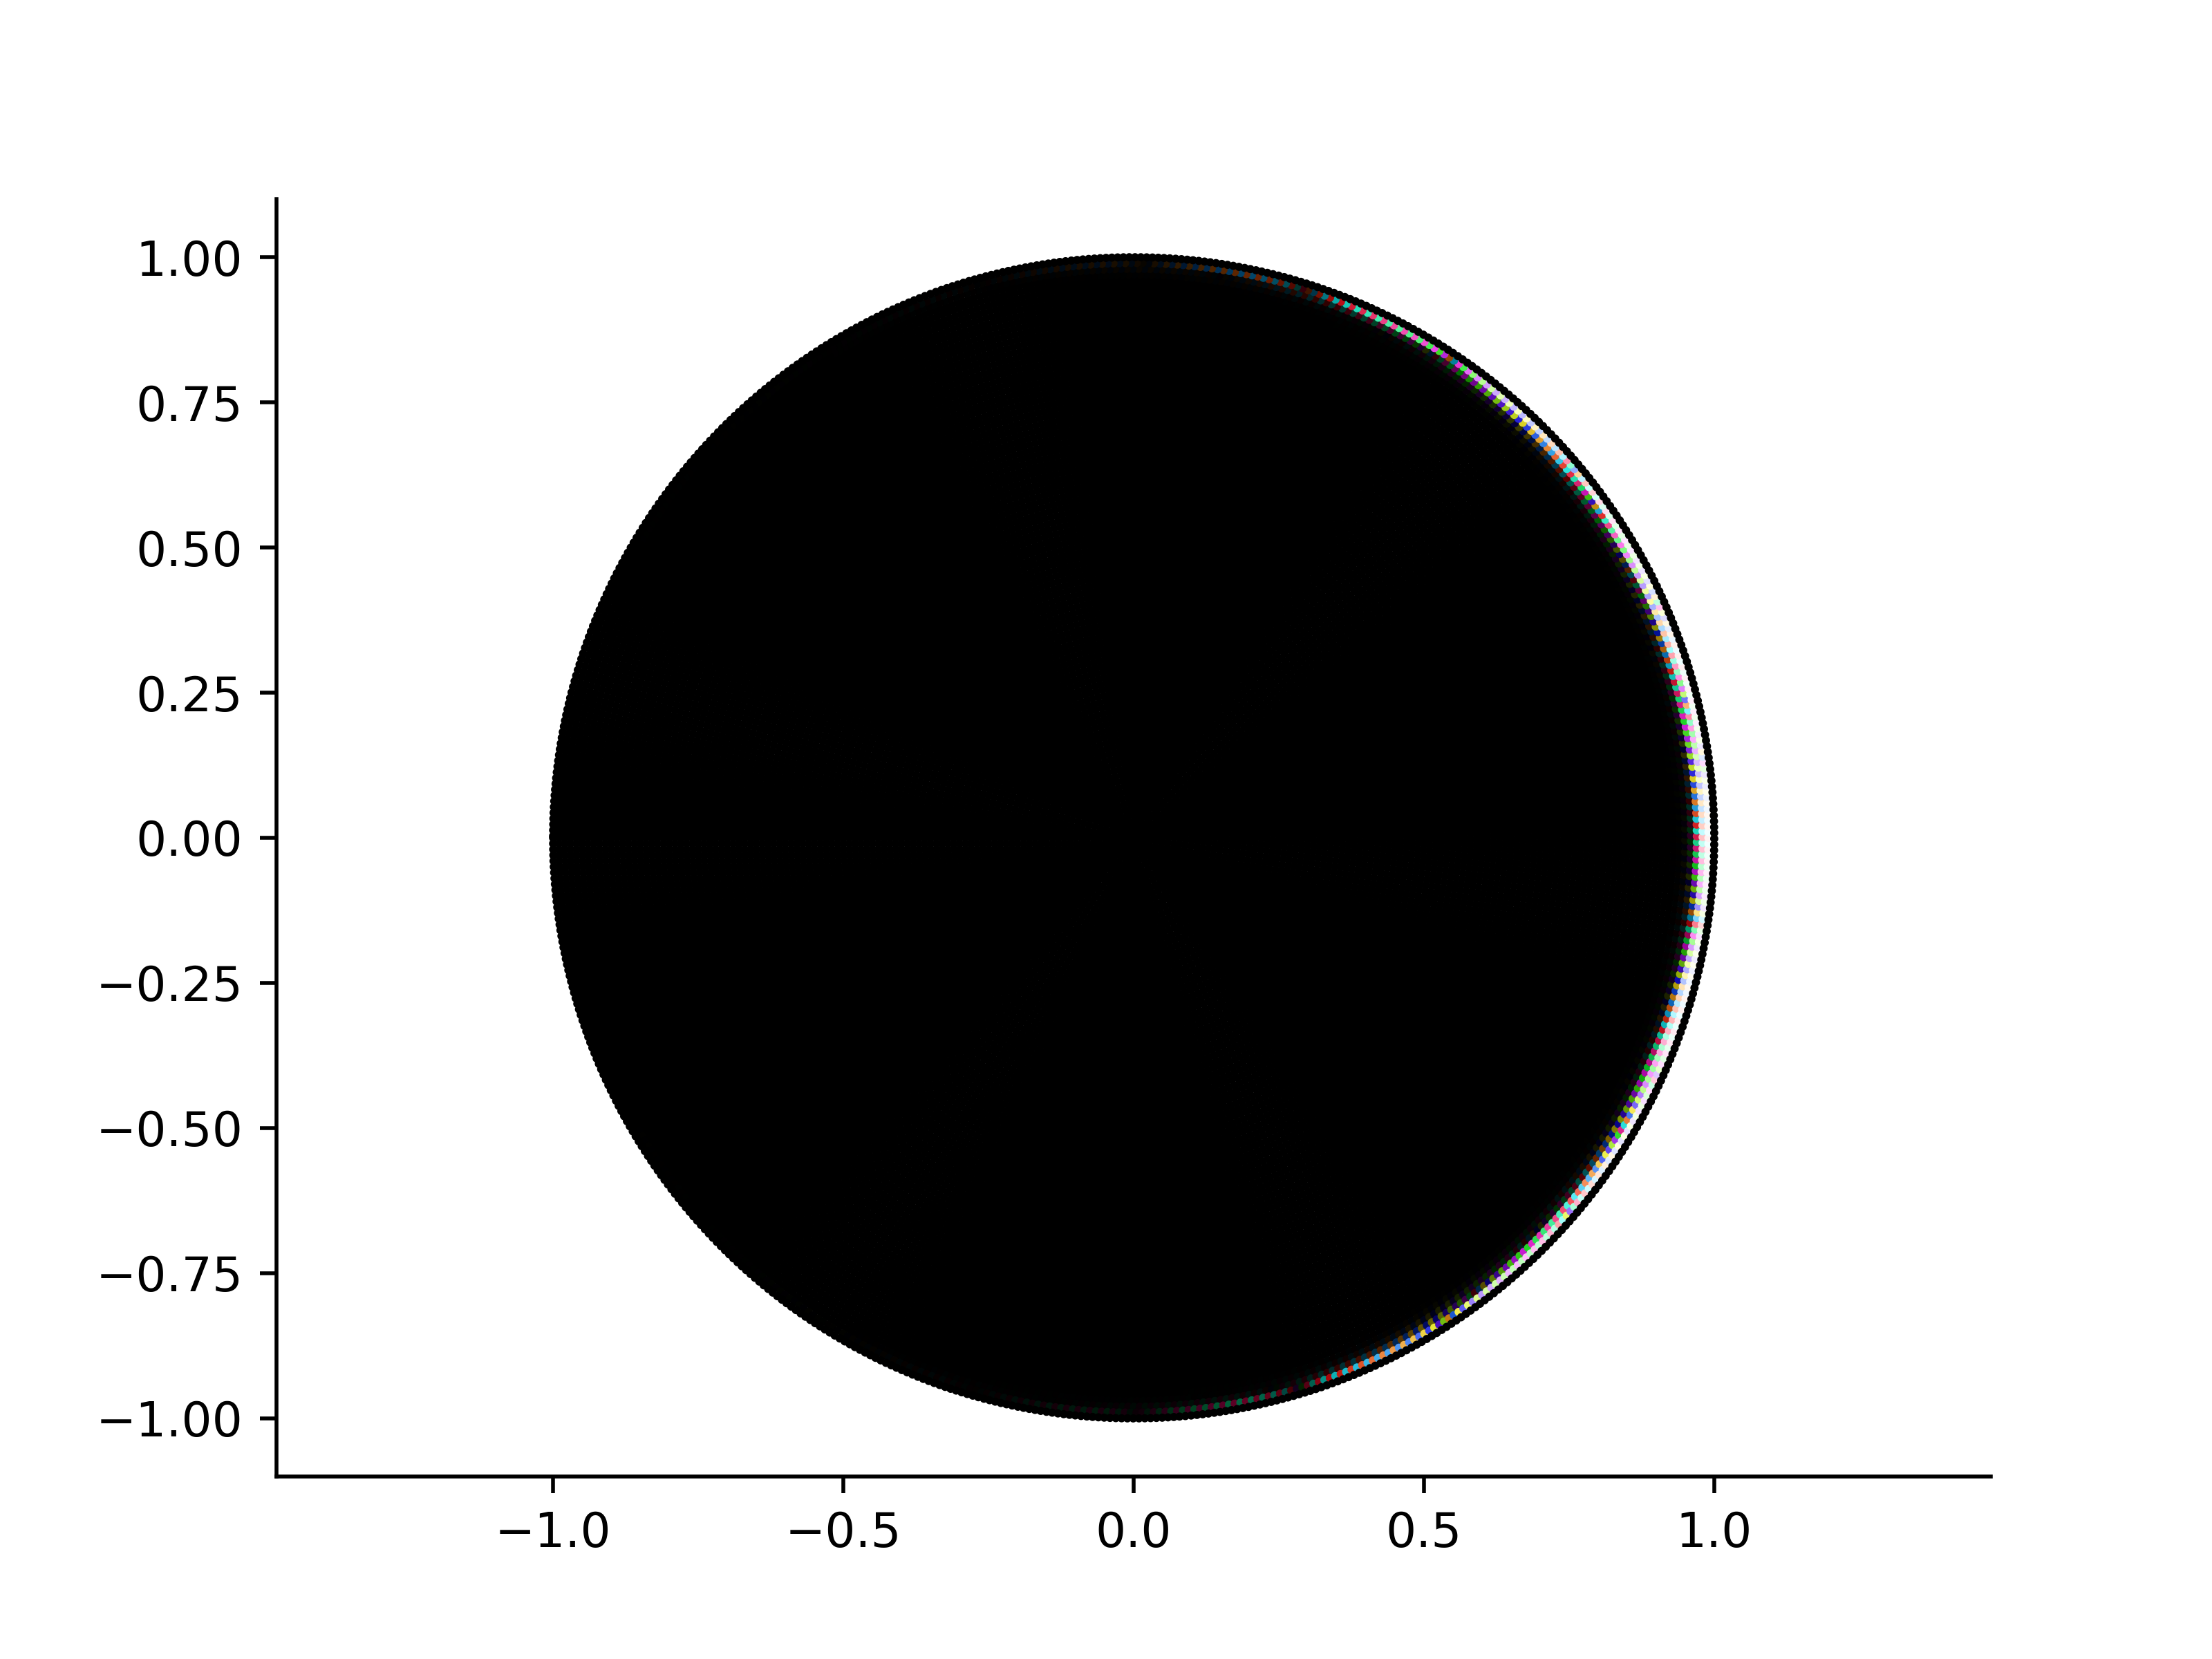
\includegraphics[width=0.7\textwidth]{../Aplicacion/diff_e^z.png}
    \caption{Diferencia entre las figuras \ref{fig:comp_e^z} y \ref{fig:e^z}.}
    \label{fig:diferencia}
\end{figure}

Como hemos comentado previamente, $f$ ha de ser continua para que se pueda extender con continuidad al disco cerrado. Pero, ¿qué pasa cuando no lo es? El resultado será una función con parte real e imaginaria armónicas en el interior (no necesariamente una conjugada de la otra) pero que no se puede prolongar con continuidad a la frontera, como es lógico. Además, si $f$ es continua a trozos, la función que se obtiene a partir de ella es armónica y continua en los puntos del borde donde lo sea $f$. \\

La figura \ref{fig:atrozos} ilustra lo que se acaba de comentar. A la izquierda se observa la extensión armónica al disco de la función $f(t) = 0$ si $- \pi < t < 0$ y $f(t) = 100$ si $0 \leq t \leq \pi$; y a la derecha se representa la extensión armónica al disco de la función $f(t) = 20i$ si $- \pi < t < 0$, $f(t) = -20$ si $0 \leq t < \frac{\pi}{2}$ y $f(t) = 20$ si $\frac{\pi}{2} \leq t \leq \pi$. \\

\begin{figure}[!htbp]
    \centering
    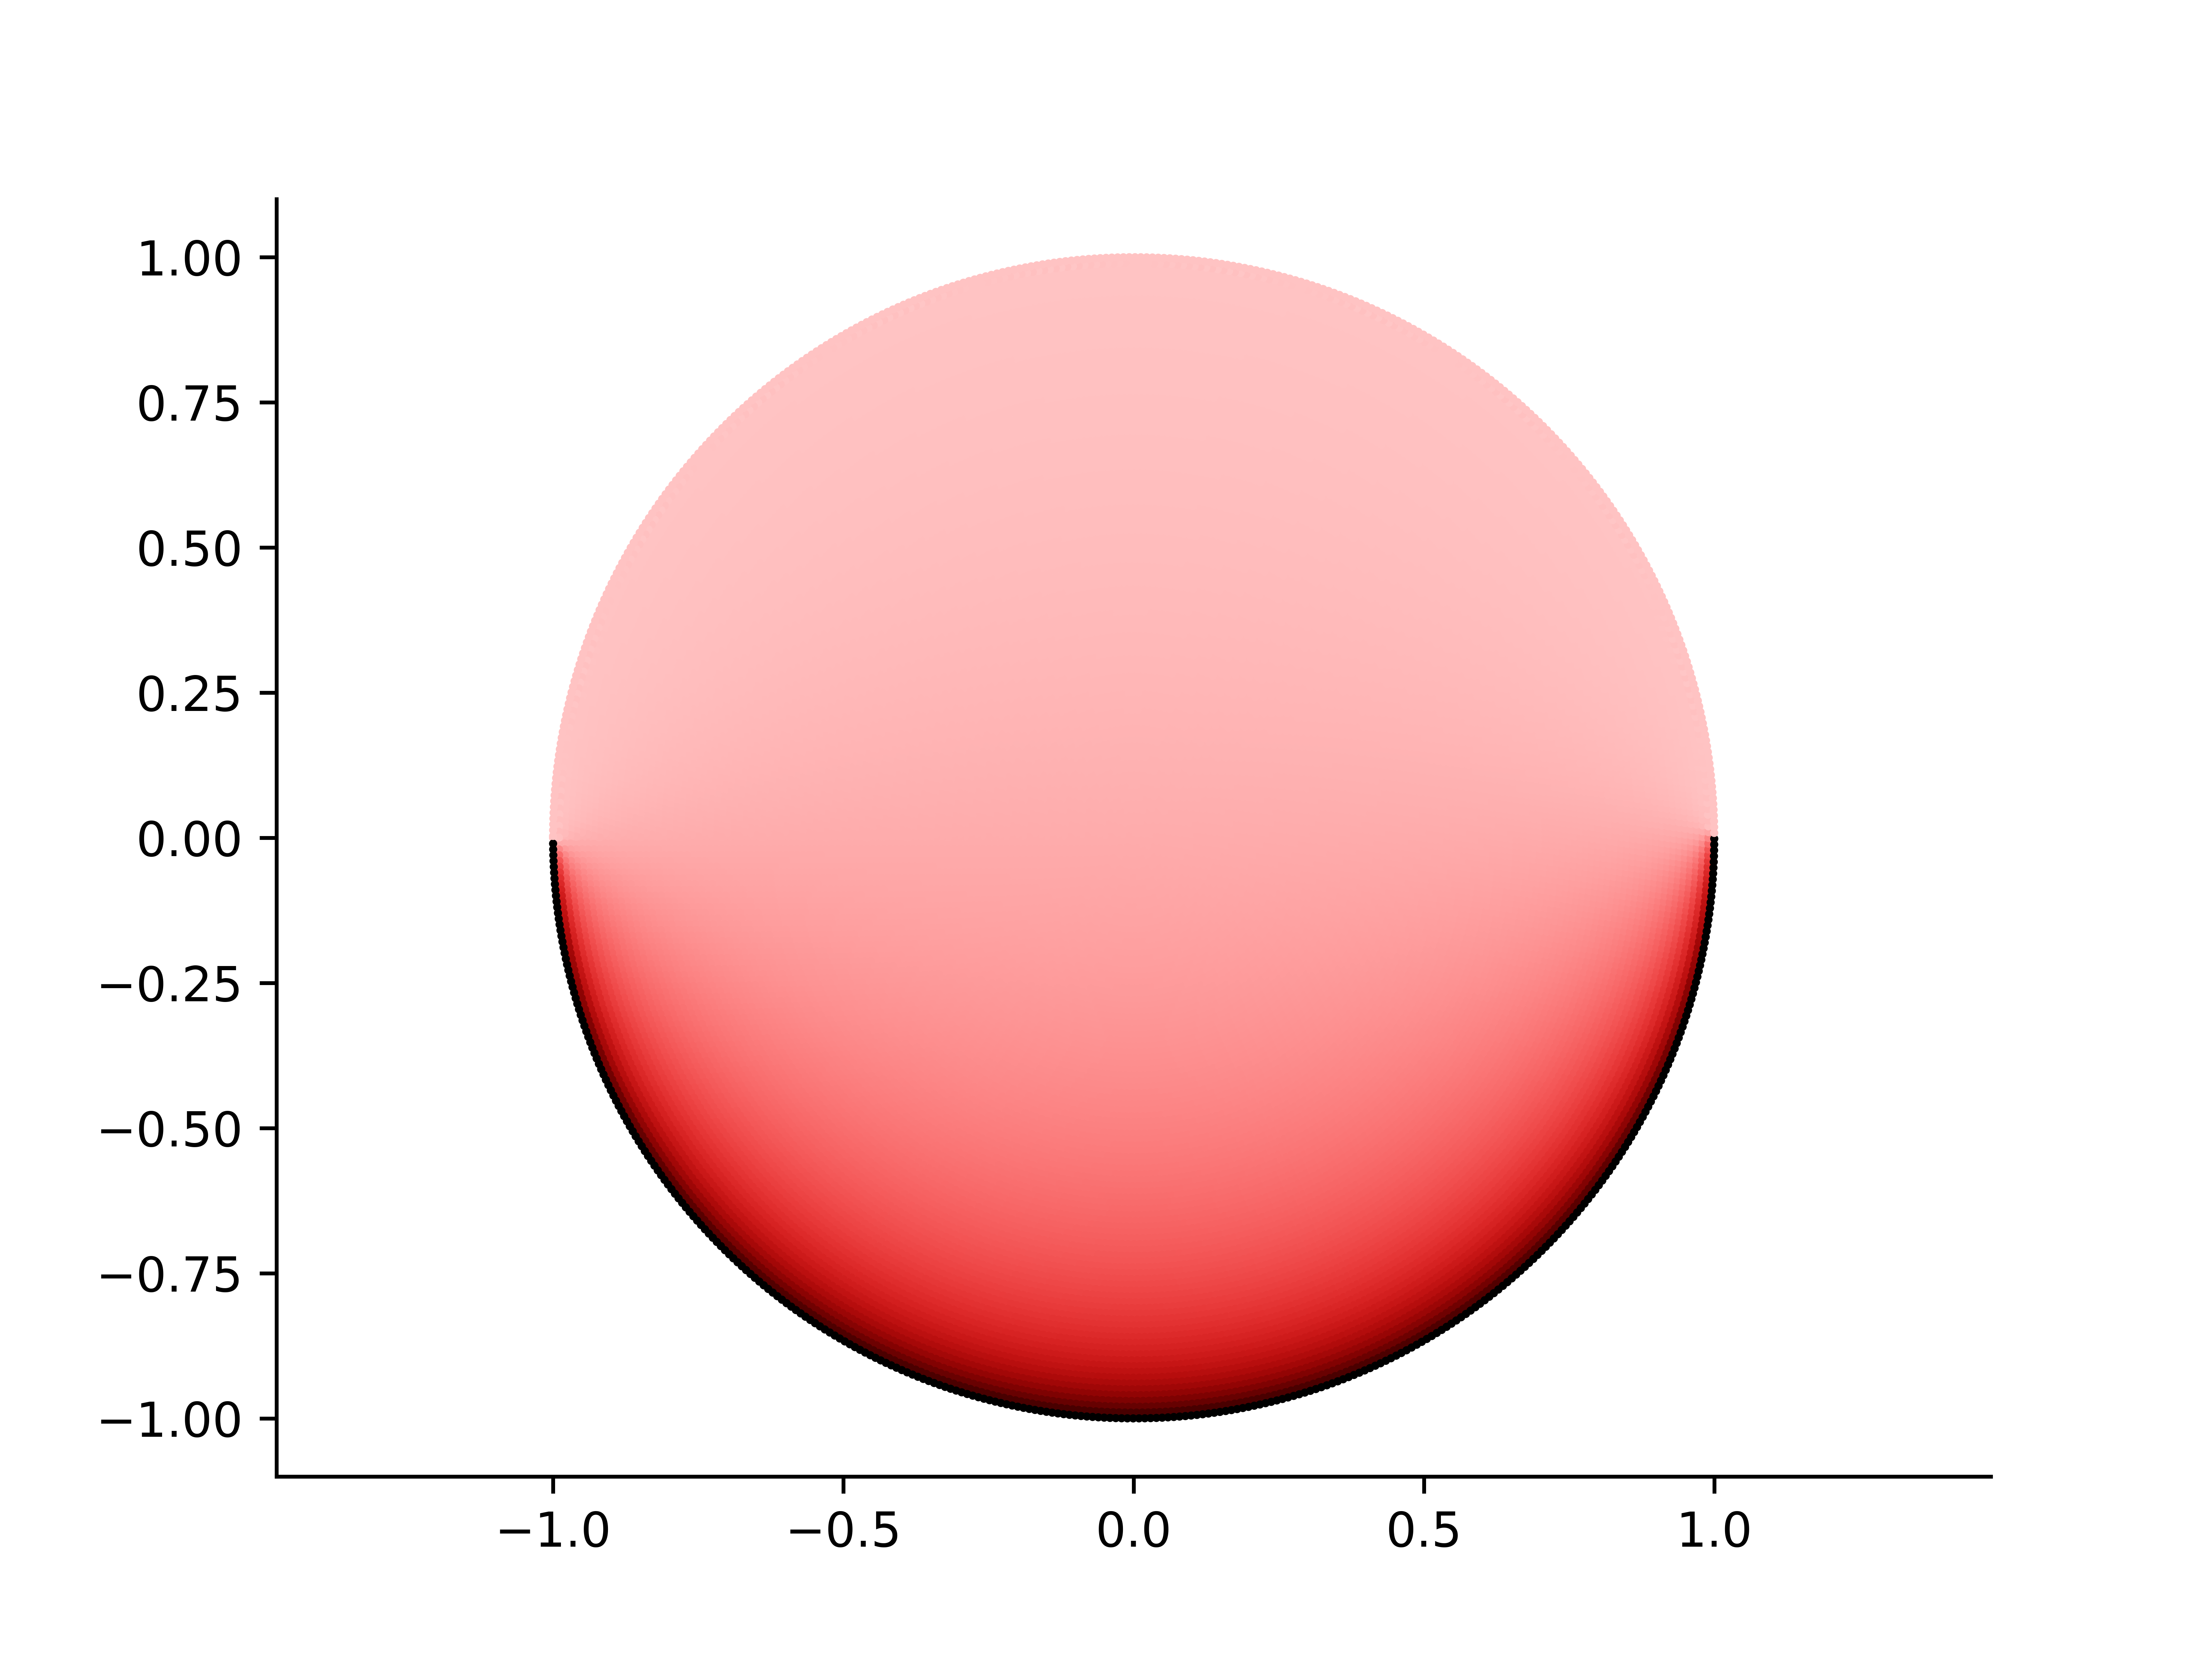
\includegraphics[width=0.49\textwidth]{../Aplicacion/atrozos.png}
    \hfil
    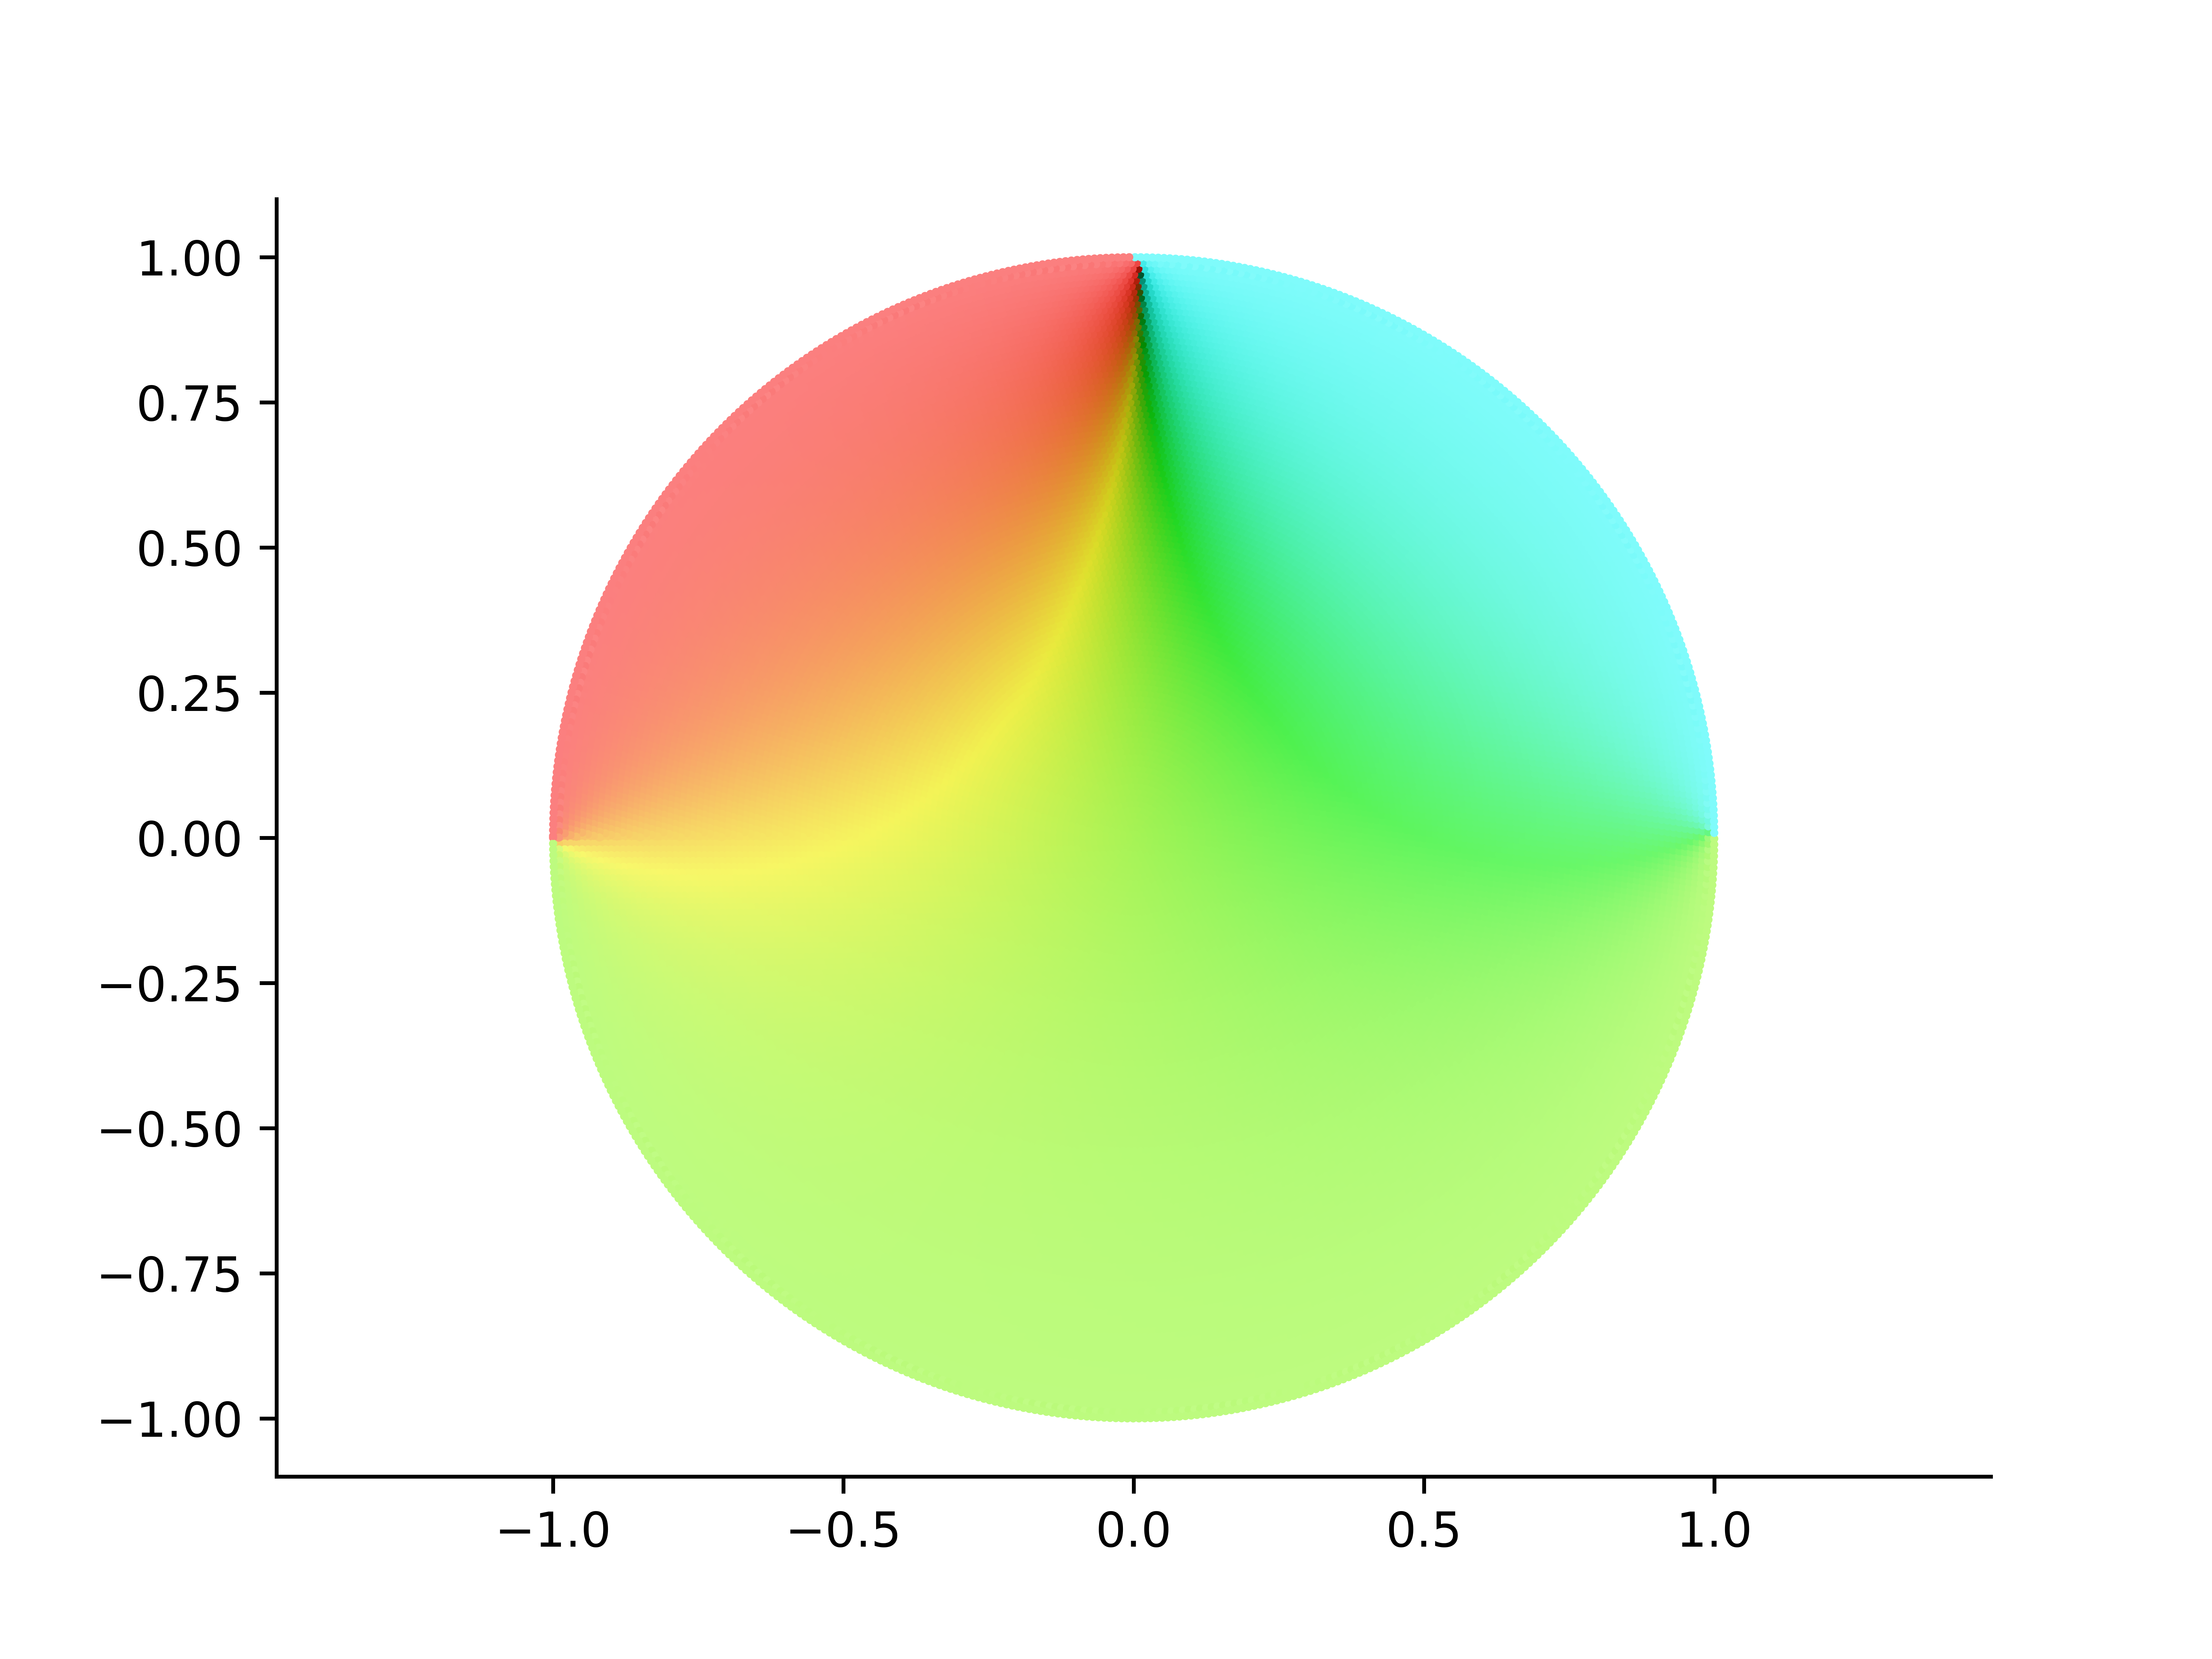
\includegraphics[width=0.49\textwidth]{../Aplicacion/atrozos(2).png}
    \caption{Funciones definidas a trozos.}
    \label{fig:atrozos}
\end{figure}


\chapter{Ejemplos}

\todo[inline]{Empezar comentando cómo calcular el radio de convergencia, que los ejemplos son de series con radio de convergencia 1 y que vas a mostrar cómo difieren el comportamiento en la frontera de unos a otros.}

En esta sección vamos a estudiar el comportamiento de algunas series de potencias en el borde de su disco de convergencia.

%%%%%%%%%%%%%%%%%%%%%%%%%%%%%%%%%%%%%%%%%%%%%%%%%%%%%%%%%%%%%%%%%%%%%%%%%%%%%%%%
%EJEMPLO 1
%%%%%%%%%%%%%%%%%%%%%%%%%%%%%%%%%%%%%%%%%%%%%%%%%%%%%%%%%%%%%%%%%%%%%%%%%%%%%%%%

\begin{example}
    Mostrar que
    \begin{equation*}
        \sum_{n=0}^{\infty} z^n, \, \abs{z} < 1
    \end{equation*}
    diverge en todo punto tal que $\abs{z} = 1$.
\end{example}

\begin{proof}
Es fácil ver que $1 - z^{n+1} = (1 - z) (1+ z + z^2 + \cdots + z^n)$. Por lo tanto, si $z \neq 1$, se tiene que
\begin{equation}
    1 + z + \cdots + z^n = \frac{1 - z^{n+1}}{1-z}.
\end{equation}

Si $\abs{z} < 1$ entonces $\lim_{n \rightarrow \infty} z^n = 0$ y la serie converge a
\begin{equation*}
    \sum_{n=0}^{\infty} z^n = \frac{1}{1 - z}
\end{equation*}

Si $\abs{z} > 1$ entonces $\lim_{n \rightarrow} z^n = \infty$ y la serie diverge. Pero, ¿qué pasa cuando $\abs{z} = 1$? La serie de potencias $\sum_{n=0}^{\infty} z^n$ diverge en todos los puntos del radio de convergencia pues $\abs{z^n}$ no tiende a 0 cuando $n \rightarrow \infty$.

Sin embargo, $\sum_{n=0}^{\infty} z^n$ puede ser extendida a la función globalmente analítica $\frac{1}{1-z}$ en $\complex \setminus \{1\}$ gracias a una cantidad finita de prolongaciones analíticas.

Tomemos $a$ un punto cualquiera de $\complex \setminus \{1\}$ y conectémoslo al origen $0$ mediante la curva de Jordan $\gamma \subset \complex \setminus \{1\}$. Fijemos un punto $z_1$ en $\gamma$ que cumpla $\abs{z} < 1$. $\sum_{n=0}^{\infty} z^n$ puede ser extendida analíticamente en $z_1$ de la siguiente forma:
\begin{equation*}
    \begin{split}
        \frac{1}{1-z} & = \frac{1}{1 - z_1 - (z - z_1)} = \frac{1}{1 - z_1} \frac{1}{1 - \frac{z - z_1}{1 - z_1}} = \frac{1}{1 - z_1} \sum_{n=0}^{\infty} \left(\frac{z - z_1}{1 - z_1} \right)^n = \\
                      & = \sum_{n=0}^{\infty}  \frac{1}{(1 - z_1)^{n+1}} (z - z_1)^n, \abs{z - z_1} < \abs{1 - z_1}.
    \end{split}
\end{equation*}

De nuevo, tomemos $z_2$ en $\gamma$ tal que $\abs{z_2 - z_1} < \abs{1 - z_1}$ y $\abs{z_2} \geq 1$. Podemos extender la serie de potencias a $z_2$.
\begin{equation*}
    \frac{1}{1-z} = \sum_{n=0}^{\infty} \frac{1}{(1 - z_2)^{n+1}} (z - z_2)^n , \abs{z - z_2} < \abs{1 - z_2}.
\end{equation*}

\todo[inline]{Hacer dibujo, como en el libro de Lin.}

Después de un número finito de iteraciones, dado que la curva es un conjunto compacto, alcanzaremos el punto $a$ y tendremos
\begin{equation*}
    \frac{1}{1-z} = \sum_{n=0}^{\infty} \frac{1}{(1 - a)^{n+1}} (z - a)^n , \abs{z - a} < \abs{1 - a}.
\end{equation*}

Así, decimos que hemos obtenido la prolongación analítica de $\sum_{n=0}^{\infty} z^n$ que pasa por la curva $\gamma$.
\end{proof}

%%%%%%%%%%%%%%%%%%%%%%%%%%%%%%%%%%%%%%%%%%%%%%%%%%%%%%%%%%%%%%%%%%%%%%%%%%%%%%%%
%EJEMPLO 2
%%%%%%%%%%%%%%%%%%%%%%%%%%%%%%%%%%%%%%%%%%%%%%%%%%%%%%%%%%%%%%%%%%%%%%%%%%%%%%%%

\begin{example}
    Mostrar que
    \begin{equation*}
        g(z) = \sum_{n=1}^{\infty} \frac{z^n}{n}, \, \abs{z} < 1
    \end{equation*}
    diverge en $z = 1$  y converge en el resto de punto tales que $\abs{z} = 1$;

\end{example}

\begin{proof}
    En primer lugar, cabe destacar que la serie armónica $\sum_{n=1}^{\infty} \frac{1}{n}$ diverge. Para demostrar que la serie diverge en $z = 1$  y converge en el resto de punto tales que $\abs{z} = 1$ vamos a aplicar el criterio de Dirichlet: \\ \par

    Sean $\{a_n\} \subset \real$ y $\{b_n\} \subset \complex$ sucesiones tales que:
    \begin{itemize}
        \item[1.] $\{a_n\}$ es monótona con límite $0$
        \item[2.] Las sumas parciales de la serie $\sum_{n=1}^{\infty} b_n$ están acotadas
    \end{itemize}
    %\begin{itemize}
    %    \item[1.] $a_1 \geq a_2 \geq \dots$
    %    \item [2.] $\lim_{n \rightarrow \infty} a_n = 0$
    %    \item[3.] Existe $M > 0$ tal que $\sum_{n=1}^{N} b_n \leq M$ para todo $N \in \naturals$
    %\end{itemize}
    entonces $\sum_{n=1}^{N} a_nb_n$ converge. \\ \par

    En nuestro caso vamos a tomar $a_n = \frac{1}{n}$ y $b_n = z^n$. La primera condición se cumple, veamos la que resta:
    \begin{equation*}
        \abs{\sum_{n=1}^{N} z^n} = \abs{\frac{z - z^{N+1}}{1 - z}} \leq \frac{2}{\abs{1 - z}}, \text{ si } z \neq 1 \text{, para todo } N \in \naturals.
    \end{equation*}

    Esto muestra que la condición se satisface para todo $z \not = 1$ en el disco unidad. Por lo tanto, la serie converge para todo $z$ tal que $\abs{z} \leq 1, z \not = 1$ y diverge para $\abs{z} > 1$. \\ \par

    Vamos a ver que la suma de la serie es $\log{\frac{1}{1 - z}}$. En efecto, derivando tenemos que
    \begin{equation*}
        g'(z) = \sum_{n=1}^{\infty} z^{n-1} \Rightarrow z g'(z) = \sum_{n=1}^{\infty} z^n = \frac{z}{1 - z}.
     \end{equation*}
     Si integramos ahora la expresión de la derecha tenemos que la suma es $\log{\frac{1}{1 - z}}$ puesto que $g(0) = 0$.

     % Puedes  añadir que un argumento análogo permite presentar ejemplos de series con disco de convergencia de radio 1, pero que divergen en una cantidad arbitraria de puntos del borde. Por ejemplo, la serie de término general z^{pn}/n, diverge en las p raíces p-ésimas de la unidad.
\end{proof}

%%%%%%%%%%%%%%%%%%%%%%%%%%%%%%%%%%%%%%%%%%%%%%%%%%%%%%%%%%%%%%%%%%%%%%%%%%%%%%%%
%EJEMPLO 3
%%%%%%%%%%%%%%%%%%%%%%%%%%%%%%%%%%%%%%%%%%%%%%%%%%%%%%%%%%%%%%%%%%%%%%%%%%%%%%%%

\begin{example}
    Mostrar que
    \begin{equation*}
        f(z) = \sum_{n=1}^{\infty} \frac{z^n}{n^2}, \, \abs{z} < 1
    \end{equation*}
    converge absoluta y uniformemente en $\abs{z} = 1$.
\end{example}

\begin{proof}
    Es fácil ver que converge absoluta y uniformemente en $\abs{z} = 1$ dado que
    \begin{equation*}
        \sum_{n=1}^{\infty} \abs{\frac{z^n}{n^2}} \leq \sum_{n=1}^{\infty} \abs{\frac{1}{n^2}} < \infty.
    \end{equation*}

    Esta función $f$ define una función holomorfa y acotada en el disco abierto $\disk$, que además es continua en el disco cerrado $\closedisk$. Sin embargo, no puede extenderse con continuidad en $z = 1$.
    \begin{equation*}
        f'(z) =  \sum_{n=1}^{\infty} \frac{z^{n-1}}{n} \Rightarrow zf'(z) = \sum_{n=1}^{\infty} \frac{z^{n}}{n} = g(z) = \log{\frac{1}{1 - z}}.
    \end{equation*}

    \begin{comment}
    \begin{equation*}
        f''(z) =  \sum_{n=2}^{\infty} \frac{(n - 1)}{n} z^{n-2} =  \sum_{n=2}^{\infty} z^{n-2} - \sum_{n=2}^{\infty} \frac{1}{n} z^{n-2}
    \end{equation*}
     \begin{equation*}
         \sum_{n=2}^{\infty} z^{n-2} = \sum_{n=0}^{\infty} z^{n} = \frac{1}{1 - z}.
    \end{equation*}
    \end{comment}

 \end{proof}

%%%%%%%%%%%%%%%%%%%%%%%%%%%%%%%%%%%%%%%%%%%%%%%%%%%%%%%%%%%%%%%%%%%%%%%%%%%%%%%%
%EJEMPLO 4
%%%%%%%%%%%%%%%%%%%%%%%%%%%%%%%%%%%%%%%%%%%%%%%%%%%%%%%%%%%%%%%%%%%%%%%%%%%%%%%%

\begin{example}
    Mostrar que la serie lagunar,
    \begin{equation*}
        h(z) = \sum_{n=0}^{\infty}  z^{2^n}, \, \abs{z} < 1
    \end{equation*}
 tiene una singularidad en cada punto tal que $\abs{z} = 1$.
\end{example}

\begin{proof}
     Sea $h(z) = \sum_{n=0}^{\infty} z^{2^n} = z + z^2 + z^4 + z^8 + \cdots$. Podemos escribir lo siguiente:
    \begin{equation*}
         h(z^2) = h(z) - z, \,
         h(z^4) = h(z^2) - z^2,
    \end{equation*}
    y aplicando inducción tenemos que
    \begin{equation*}
        h(z^{2^k}) = h(z^{2^{k-1}}) - z^{2^{k-1}}
    \end{equation*}

    Así,
    \begin{equation*}
        h(z) = z + h(z^2) = z + z^2 + h(z^4) = \cdots = z + z^2 + \cdots + z^{2^{k-1}} + h(z^{2^k}).
    \end{equation*}

    Si $m, n \in \naturals$ y $r \in (0,1)$ y llamamos $r$ a $e^{2 \pi i \frac{m}{2^n}}$, tenemos que
    \begin{equation*}
        h(r^{2^n}) = \sum_{k=0}^{\infty} (r^{2^n})^{2^k} = \sum_{k=0}^{\infty} r^{2^n \cdot 2^k} = \sum_{k=0}^{\infty} r^{2^{(n+k)}} =  \sum_{k=n}^{\infty} r^{2^k}.
    \end{equation*}

    Como
    \begin{equation*}
        \sum_{k=n}^{\infty} r^{2^k} \geq \sum_{k=n}^{N} r^{2^k} > (N + 1) r^{2^k} \rightarrow N + 1,
    \end{equation*}

    entonces $\lim_{r \rightarrow 1} \abs{h(re^{2 \pi i \frac{m}{2^n}})} = \infty \, \, \forall m, n$. \\ \par

    Puesto que $\{e^{2 \pi i \frac{m}{2^n}} : m, n \in \naturals\}$ es denso en $\partial \disk$, todos los puntos del borde del disco unidad son singulares.
\end{proof}


\begin{example}
    Mostrar que la función
    \begin{equation*}
        f(z) = \exp{\left(\frac{z + 1}{z - 1}\right)}, \, z \in \disk
    \end{equation*}
    es holomorfa, $\abs{f(z)} \leq 1$ para todo $z \in \disk$, y $f(t) \rightarrow 0$ cuando $t \rightarrow 1^-$.
\end{example}

\begin{proof}
    La función $f$ es holomorfa ya que es la composición de funciones holomorfas. Obsérvese que el único punto singular es $z = 1$.

    La función $g(z) = \frac{z + 1}{z - 1}$ lleva el disco en el semiplano $H = \{w: \Re (w) < 0\}$. Así pues, la exponencial lleva $H$ en $\disk$:
    \begin{equation*}
        \abs{e^z} = \abs{e^{x+iy}} = \abs{e^{x}(\cos y + i\sen y)} = e^{x} < 1.
    \end{equation*}

    La aplicación $g$ es una transformación de Möbius, y las transformaciones de Möbius tienen la propiedad de que llevan circunferencias y rectas en circunferencias y rectas. Como la función lleva $-1$ a $0$, $i$ a $-i$ y $-i$ a $i$, la imagen del círculo $\abs{z}=1$, ha de ser una recta. \\

    Si tomamos una sucesión $\{t_n\}$ en el intervalo $(-1,1)$ que converge a $1$, se tiene que $g(t_n) \to - \infty$. Por lo tanto,
    \begin{equation*}
        \frac{t + 1}{t - 1} \xrightarrow[t \rightarrow 1^-]{}  - \infty \Rightarrow \exp \left(  \frac{t + 1}{t - 1} \right) \xrightarrow[t \rightarrow 1^-]{} 0.
    \end{equation*}

    Sin embargo, la función $f$ no tiene límite en $1$. Por ejemplo, si tomamos la sucesión $\{z_n\}$ definida por $z_n = g(w_n)$, siendo $\{w_n\}$ la sucesión de término general $-1 + 2n \pi i$. Entonces,
     \begin{equation*}
         z_n = \frac{2n \pi i}{-2 + 2n \pi i} = \frac{n \pi i}{n \pi i - 1} =  \frac{(n \pi i + 1) n \pi i}{- n^2 \pi^2 - 1} = \frac{-n^2 \pi^2 + i n \pi}{-n^2 \pi^2 - 1}.
     \end{equation*}

     Como $g = g^{-1}$ tenemos
     \begin{equation*}
         e^{g(z_n)} = e^{w_n} \rightarrow e^{-1} \not = 0.
     \end{equation*}

     \todo[inline]{Extender este ejemplo con lo que hemos visto en el capítulo de espacios de Banach.}
\end{proof}

\chapter{$\bholomorphic{\disk}$ como álgebra de Banach}

En este capítulo vamos a trabajar con $\bholomorphic{\disk}$ como el álgebra de las funciones holomorfas acotadas en el disco unidad. \\

\begin{definition}
    Un espacio vectorial complejo se denomina espacio de Banach si es normado y completo.
\end{definition}

\medskip
$\bholomorphic{\disk}$ es un espacio vectorial complejo, que dotado con la norma infinito
\begin{equation*}
    \norminf{f} = \sup_{\abs{z} < 1} \abs{f(z)},
\end{equation*}
es un espacio vectorial normado y completo sobre $\complex$. Atendiendo a la definición anterior, decimos que  $(\bholomorphic{\disk}, \norminf{\cdot})$ es un espacio de Banach. \\

\begin{definition}
    Decimos que $B$ es un álgebra de Banach si es un espacio de Banach con un álgebra asociada tal que la multiplicación satisface:
    \begin{equation*}
        \forall x, y \in B: \, \norm{x \cdot y} \leq \norm{x} \cdot \norm{y}.
    \end{equation*}
\end{definition}

\medskip
También podemos ver $\bholomorphic{\disk}$ como un álgebra. En efecto, si $f, g \in \bholomorphic{\disk}$ y $\alpha, \beta \in \complex$, entonces
\begin{equation*}
    \begin{split}
        & \alpha f + \beta g \in \bholomorphic{\disk} \\
        & fg \in \bholomorphic{\disk}.
    \end{split}
\end{equation*}

Así, $\bholomorphic{\disk}$ es un álgebra de Banach conmutativa (con la función constante 1 como elemento unidad) puesto que es un álgebra conmutativa y un espacio de Banach cuya norma asociada cumple la siguiente propiedad:
\begin{equation*}
    \forall f, g \in \bholomorphic{\disk}: \, \norminf{f \cdot g} \leq \norminf{f} \cdot \norminf{g}.
\end{equation*} \\

\begin{definition}
    Sea $B$ un espacio de Banach. Consideramos $B^*$ el espacio de las aplicaciones $\varphi: B \rightarrow \complex$ continuas. $B^*$ es un espacio vectorial y tiene una norma natural dada por:
    \begin{equation*}
        \norm{\varphi} = \sup_{\norm{x} \leq 1} \abs{\varphi(x)}.
    \end{equation*}
    Con esta norma, $B^*$ es un espacio de Banach al que llamamos espacio conjugado de $B$.
\end{definition}

\medskip
Además de la topología inducida por la norma en el espacio conjugado $B^*$, vamos a considerar otra topología denominada topología débil-* en $B^*$. Está definida de la siguiente manera. Sea $\varphi_0 \in B^*$ y tomemos una cantidad finita de elementos $x_1, \dots x_n \in B$ y $\varepsilon > 0$. Sea
\begin{equation*}
U = \{ \varphi \in B^*: \abs{\varphi(x_k) - \varphi_0 (x_k)} < \varepsilon, k = 1, \dots, n\}.
\end{equation*}
un entorno $\varphi_0$. Un abierto de esta topología será, por tanto, cualquier unión de tales entornos $U$.

Es la topología más débil de $B^*$ tal que todas las funciones $\varphi \rightarrow \varphi(x)$ son continuas de $B^*$ en $\complex$, con $x \in B$. Esta topología se denota por $\sigma(B^*, B)$. % La topología débil-* es la más débil de $B^*$, es decir, es aquella que tiene el menor número de abiertos.

\begin{obs}
    El disco unidad cerrado de $B^*$ es compacto en la topología débil-*.
\end{obs}
\bigskip

Recordemos que $\phi : \bholomorphic{\disk} \rightarrow \complex$ es un homomorfismo de álgebras si para todos $f, g \in \bholomorphic{\disk}$ y $\alpha, \beta \in \complex$ se cumple:
\begin{equation}
    \begin{split}
        & \phi (\alpha f + \beta g) = \alpha \phi(f) + \beta \phi(g) \\
        & \phi(f \cdot g) = \phi(f) \cdot \phi(g).
    \end{split}
\end{equation}

El espectro de $\bholomorphic{\disk}$, denotado por $\fiber = \fiber (\bholomorphic{\disk})$, es el espacio de los homomorfismos $\phi: \bholomorphic{\disk} \rightarrow \complex$ no nulos. Observamos que tales homomorfismos verifican que $\norm{\phi} = 1$ y son continuos.\\

$\fiber$ es un subconjunto del espacio conjugado $\bholomorphic{\disk}^*$ y, de hecho, está contenido en el disco unidad de $\bholomorphic{\disk}^*$. Además, $\fiber$ es cerrado en la topología débil estrella en $B^*$. \\

Como el disco unidad en $\bholomorphic{\disk}^*$ equipado con la topología débil-* es compacto, se sigue que $\fiber$ (como subconjunto de $\bholomorphic{\disk}^*$) equipado con la topología débil estrella es un espacio Hausdorff compacto. ? \\

En este punto queremos asociar cada elemento de $x$ de $B$ con uno que estará sobre $\fiber(B)$. Para ello vamos a definir la siguiente aplicación:
\begin{equation*}
    \begin{split}
        \widehat x:  \fiber(B) & \rightarrow  \complex \\
                 \varphi \, \, \, & \mapsto  \varphi (x).
    \end{split}
\end{equation*}

Cada $\widehat x$ es una función continua en $\fiber (B)$. De hecho, por definición, la topología débil-* es la topología más débil de $\fiber (B)$ que hace que cada $\widehat x$ sea continua. Así pues, tenemos la siguiente representación a la que se le suele denominar \textbf{transformada de Gelfand}
\begin{equation*}
    x \rightarrow \widehat x.
\end{equation*}
La imagen de $B$ bajo este homomorfismo es el álgebra $\widehat B = \{\widehat x: \fiber(B) \rightarrow  \complex \mid x \in B\}$. \\

Lo que hemos comentado puede aplicarse a $\bholomorphic{\disk}$. Así tenemos la siguiente aplicación
\begin{equation*}
    \begin{split}
        \widehat f:  \fiber & \rightarrow  \complex \\
                \phi \, & \mapsto  \phi (f),
    \end{split}
\end{equation*}
con $x \in \bholomorphic{\disk}$, que da lugar a la representación $f \rightarrow \widehat f$. Vamos a poder interpretar $\bholomorphic{\disk}$ como el álgebra de las funciones continuas en el espacio compacto de los ideales maximales $\fiber$. Hay que hablar más de la relación de $\fiber$ y los ideales maximales. \\

Quizá es mejor hablar primero de la transformada de Gelfand y luego introducir la topología débil-* en $\fiber$. \\

Al espacio $\fiber$ se le suele llamar el espacio de ideales maximales de $\bholomorphic{\disk}$. Para cada $\phi \in \fiber$, el kernel de $\phi$ es un ideal maximal en el álgebra $\bholomorphic{\disk}$. Recíprocamente, todo ideal maximal en $\bholomorphic{\disk}$ se corresponde con el núcleo de un homomorfismo en $fiber$. Vamos a estudiar la estructura de este espacio. \\

Los únicos homomorfismos complejos evidentes de $\bholomorphic{\disk}$ son las evaluaciones
\begin{equation*}
    \delta_z (f) = f(z).
\end{equation*}

Hablar más de las evaluaciones.

Existe una aplicación continua que lleva $\fiber$ en el disco unidad cerrado. Si denotamos por $\id$ la función identidad de $\disk$,
\begin{equation*}
    \id(z) = z, z \in \disk,
\end{equation*}
la proyección que buscamos lleva los homomorfismos $\phi \in \fiber$ en su correspondiente valor en la función $\id$. Así pues, la aplicación que nos interesa es $\widehat \id$. Para evitar confusiones, vamos a introducir una notación alternativa para referirnos a la función $\widehat \id$. Si $\phi \in \fiber$,
\begin{equation}
    \label{proyeccion}
    \begin{split}
        \pi: \fiber & \rightarrow \closedisk \\
            \phi \, & \mapsto  \phi (\id).
    \end{split}
\end{equation}

\begin{theorem}
    La aplicación $\pi: \fiber \rightarrow \closedisk$ definida por \ref{proyeccion} es continua. $\pi$ es inyectiva sobre el disco abierto $\disk$ y $\pi^{-1}$ aplica homeomorficamente $\disk$ sobre un abierto de $\fiber$.
\end{theorem}

En esta prueba llamo $\lambda$ a los puntos del disco y $z$ a la variable de la función $f$.

\begin{proof}
$\pi$ es continua por definición. Veamos que $\pi$ lleva $\fiber$ en el disco cerrado. En efecto, ya hemos observado antes que cada punto del disco abierto $\disk$ está en la imagen de $\pi$ puesto que $\pi (\phi_\lambda) = \lambda$. Como $\fiber$ es un conjunto compacto que contiene a $\disk$, y la imagen de un compacto por una aplicación continua es también un compacto, entonces $\pi(\fiber)$ es compacto. Así pues, como $\pi(\fiber)$ es un conjunto compacto que contiene a $\disk$, contiene todo el disco cerrado $\closedisk$. \\

Veamos ahora que $\pi$ es inyectiva sobre el disco. Para ello supongamos que $\abs{\lambda} < 1$ y $\pi (\phi) = \phi (\id) = \lambda$, con $\phi \in \fiber$. Si $f(\lambda) = 0$, entonces $f(z) = (z - \lambda) g(z)$ y
\begin{equation*}
    \phi(f) = \phi(z - \lambda) \phi(f) = 0 \cdot \phi(f) = 0.
\end{equation*}

Si $f(\lambda) = c$, entonces $f(z) = c + g(z)$, con $g(z) = 0$ y
\begin{equation*}
    \phi(f) = \phi(c) + \phi(g) = c + 0 = c.
\end{equation*}
Por lo tanto, $\phi(f) = f(\lambda)$ para toda $f \in \bholomorphic{\disk}$, es decir, $\phi$ es la evaluación en $\lambda$. Esto prueba que $\pi$ es inyectiva sobre los puntos del disco unidad $\disk$. \\

Si tomamos $\Delta = \pi^{-1} (\disk) = \{\phi_z : z \in \disk\}$, entonces $\pi$ lleva $\Delta$ homeomorficamente en el disco $\disk$ ya que la topología de $\Delta$ es la topología débil definida por las aplicaciones $\widehat f$ y la topología de $\disk$ es la topología débil definida por las aplicaciones $f \in \bholomorphic{\disk}$. ?\\
\end{proof}

Si $\abs{\alpha} = 1$, decimos que $\pi^{-1} (\alpha)$ es la fibra de $\fiber$ sobre $\alpha$ y lo denotamos por $\fiber_\alpha$:
\begin{equation*}
    \fiber_\alpha = \pi^{-1} (\alpha) = \{\phi \in \fiber : \phi (\id) = \alpha\}.
\end{equation*}

La fibra $\fiber_\alpha$ es un conjunto cerrado de $\fiber$. Intuitivamente, los elementos de $\fiber_\alpha$ son los homomorfismos complejos de $\fiber$ que se comportan como la ``evaluación en $\alpha$'', es decir, los homomorfismos $\phi \in \bholomorphic{\disk}$ que llevan cada $f \in \bholomorphic{\disk}$ en algo parecido al valor límite $f(z)$ cuando $z$ se aproxima a $\alpha$. Vamos a ver esto con más detalle a continuación. \\

\begin{comment}
Existe una correspondencia uno a uno entre los homomorfismos $\phi: \bholomorphic{\disk} \rightarrow \complex$ y los ideales maximales $M$ en el álgebra $\bholomorphic{\disk}$. Esta correspondencia está definida por $M = \ker (\phi)$. Cada ideal maximal $M$ es cerrado, así que cada homomorfismo $\phi$ es continuo:
\begin{equation*}
    \abs{\phi (x)} \leq \norm{x}.
\end{equation*}
\end{comment}

%Observemos que la imagen de toda función constante por cualquier elemento del espectro es ella misma. Además, la identidad es una función de $\bholomorphic{\disk}$ de norma 1. \\

\begin{theorem}
    \label{result1}
    Sea $f$ una función en $\bholomorphic{\disk}$ y sea $\alpha$ un punto del círculo unidad. Sea $\{z_n\}$ una sucesión de puntos en el disco unidad $\disk$ que converge a $\alpha$, y supongamos que el límite
    \begin{equation*}
        \zeta = \lim_{n \rightarrow \infty} f(z_n)
    \end{equation*}
    existe. Entonces existe un homomorfismo complejo $\phi$ en la fibra $\fiber_\alpha$ tal que $\phi(f) = \zeta$.
\end{theorem}

\begin{proof}
    Sea $J = \{h\in \bholomorphic{\disk} : \lim_{n \rightarrow \infty} h(z_n) = 0 \}$ un ideal propio en $\bholomorphic{\disk}$. $J$ está contenido en un ideal maximal $M$, esto es, existe un homomorfismo complejo $\phi$ de  $\bholomorphic{\disk}$ del que $M$ es el núcleo. En particular, $\phi(h) = 0$ para todo $h \in J$. Las funciones $(z - \alpha)$ y $(f - \zeta)$ están ambas en $J$. Entonces, $\phi(z) = \alpha$ y $\phi(f) = \zeta$. Por lo tanto $\phi$ es el homomorfismo buscado. \\ %Aquí se usa que \phi(c)=c, siendo c una constante.
\end{proof}

\begin{theorem}
    Sea $f$ una función en $\bholomorphic{\disk}$ y sea $\alpha$ un punto del círculo unidad. La función $\widehat f$ es constante en la fibra $\fiber_\alpha$ si y solo si $f$ se puede extender con continuidad a $\disk \cup \{\alpha\}.$
\end{theorem}

\begin{proof}
    Supongamos primero que $f$ se puede extender con continuidad a $\disk \cup \{ \alpha\}$. Esto significa que existe un número complejo $\zeta$ tal que $\lim_{z_n \rightarrow \alpha} f(z_n) = \zeta$ para toda sucesión $\{z_n\}$ en $\disk$ que converge a $\alpha$. Queremos mostrar que $\widehat f$ vale constantemente $\zeta$ en la fibra $\fiber_\alpha$, es decir, $\phi(f) = \zeta$ para todo $\phi \in \fiber_\alpha$. \\

    Podemos suponer que $\zeta = 0$. Sea $h(z) = \frac{1}{2} (1 + z \alpha^{-1})$, así que $h(\alpha) = 1$ y $\abs{h} < 1$ en cualquier otro lugar dentro del disco unidad cerrado. Como $f$ es continua en $\alpha$ y toma el valor $0$, es fácil ver que $(1 - h^n) f$ converge uniformemente a $f$ cuando $n \rightarrow \infty$. Si $\phi$ es un homomorfismo complejo de $\bholomorphic{\disk}$ que yace en la fibra $\fiber_\alpha$, es decir, $\phi (z) = \alpha$, entonces $\phi (h) = 1$. Por lo tanto, $\phi [(1 - h^n)f] = 0$, y, como $\phi$ es continua, $\phi (f) = 0$. Así, $\widehat f$ es la función idénticamente nula en $\fiber_\alpha$. \\

    %Si $\widehat f$ vale constantemente $\zeta$ en la fibra $\fiber_\alpha$, entonces el Teorema \ref{result1} implica que $f(z) \rightarrow \zeta$ cuando $z_n \rightarrow \alpha$. Si definimos $f (\alpha) = \zeta$, entonces $f$ se puede extender con continuidad a $\disk \cup \{ \alpha \}$.

    Si $\widehat f$ es constante en la fibra $\fiber_\alpha$, entonces el Teorema \ref{result1} muestra directamente que $f$ se puede extender con continuidad a $\disk \cup \{ \alpha \}$. \\
\end{proof}

%\bigskip
%La discusión anterior muestra que $\disk \in \fiber (\bholomorphic{\disk})$. Entonces podemos definir la corona de $\bholomorphic{\disk}$ como $\fiber (\bholomorphic{\disk}) \setminus \disk$.

Podemos ahora hacernos algunas preguntas de carácter topológico sobre el espacio de ideales maximales de $\bholomorphic{\disk}$. Las evaluaciones punto a punto llevan el disco unidad abierto en un conjunto abierto $\Delta$ de $\fiber$. El resto de homomorfismos yacen en las fibras $\fiber_\alpha$ y son límites de los puntos de $\Delta$. La cuestión que nos planteamos es la siguiente: ¿son esos homomorfismos realmente límites de $\phi_z$ en la topología de $\fiber$? En otras palabras, ¿es el disco $\disk$ denso en $\fiber$? A esta pregunta se le ha denominado El Problema de la Corona. \\

\begin{theorem}[Teorema de la Corona]
    El problema de la corona es equivalente a:
     Sean $f_1, \dots, f_n \in \bholomorphic{\disk}$ y $\delta > 0$ tales que para cada $z \in \disk$ se tiene
\begin{equation*}
    \abs{f_1(z)} + \cdots + \abs{f_n(z)} \geq \delta,
\end{equation*}
     entonces existen $g_1, \dots, g_n \in \bholomorphic{\disk}$ tales que $f_1 g_1 + \cdots + f_n g_n = 1$.

    %Si $\phi \in \fiber \exists (z_\alpha) \subset \disk / \forall g \in \bholomorphic{\disk} \lim_\alpha g(z_\alpha) = \widehat g(\phi) = \phi (g)$, siendo $g(z_\alpha) = \delta_{z_\alpha} (g)$.
\end{theorem}

\begin{proof}
Supongamos que $\disk$ es denso. Sean $f_1, \dots, f_n \in \bholomorphic{\disk}$ y $\delta > 0$ tales que para cada $z \in \disk$ se tiene
\begin{equation*}
    \abs{f_1(z)} + \cdots + \abs{f_n(z)} \geq \delta.
\end{equation*}

Si la función constante $1$ no se pudiera escribir de la forma $f_1 g_1 + \cdots + f_n g_n$, con $g_1, \dots, g_n \in \bholomorphic{\disk}$, tomemos $\phi \in \fiber$ no nulo tal que el ideal maximal $\ker \phi$ contiene al ideal propio generado por $f_1, \dots, f_n$.

Como $\disk$ es denso en $\fiber$ para $w^*$, existe una red $\{z_\alpha \} \subset \disk$ que tiende $w^*$ a $\phi$. En particular, para cada $f_j$ se tiene que $\lim_\alpha f_j (z_\alpha) = \widehat{f_j} (\phi) = 0, 1 \leq j \leq n$. Esto contradice la acotación relativa a $\abs{f_1(z)} + \cdots + \abs{f_n(z)}$. \\

Recíprocamente, supongamos que $\disk$ no es denso en $\fiber$, entonces existe un elemento no nulo $\phi_0 \in \fiber$ que no está en la adherencia de $\disk$. Por definición de la topología de $\fiber$, existen funciones $f_1, \dots, f_n \in \bholomorphic{\disk}$ y $\delta > 0$ tales que $\phi_0 (f_j) = 0, j = 1, \dots, n$ y el abierto
\begin{equation*}
    \{ \phi \in \fiber : \abs{\phi (f_j)} < \delta, 1 \leq j \leq n \}
\end{equation*}
no corta a $\disk$. En particular, para cada $z \in \disk$ se cumple que
\begin{equation*}
    \abs{f_1(z)} + \cdots + \abs{f_n(z)} \geq \delta
\end{equation*}
y las funciones $f_1, \dots, f_n$ están en un ideal propio de $J \subset \bholomorphic{\disk}$ ya que $J \subset \ker \phi_0$. %Esto es porque $\phi_0 (f_j) = 0$

La afirmación de que $f_1, \dots, f_n$ están en un ideal propio es equivalente a la afirmación de que la función constante $1$ no se puede escribir de la forma $f_1 g_1 + \cdots + f_n g_n = 1$, con $g_1, \dots, g_n \in \bholomorphic{\disk}$, ya que $\phi (1) = 1$ y $\phi (f_1 g_1 + \cdots + f_n g_n) = \phi (f_1) \phi (g_1) + \cdots + \phi (f_n) \phi (g_n) = 0$. \\
\end{proof}

\begin{prop}
    Para todo $f \in \bholomorphic{\disk}$ y $\alpha$ tal que $\abs{\alpha} = 1$ se cumple que
    \begin{equation*}
        \widehat{f} (\fiber_\alpha) \subset Cl(f, \alpha).
    \end{equation*}
\end{prop}

\begin{proof}
    Sea $\phi \in \fiber_\alpha$. Veamos que existe una sucesión $\{ z_n\} \subset \disk$ tal que
    \usetagform{roman} \leqnomode
    \begin{align}
        & \lim_{n \rightarrow \infty} z_n = \alpha \\
        & \lim_{n \rightarrow \infty} f(z_n)= \widehat{f} (\phi).
    \end{align}

    Como $\disk$ es denso en $\fiber$ para $w^*$, se cumple que existe $\{z_\alpha\} \subset \disk$ tal que $\delta_{z_\alpha} \rightarrow \phi$. Es decir, para toda función $h \in \bholomorphic{\disk}$ se tiene que $h (z_\alpha) \rightarrow \widehat{h} (\phi)$. En particular, para $g(z) = z$ es cierto por lo que, como $\phi \in \fiber_\alpha$, tenemos
    \begin{equation*}
        g(z_\alpha) = z_\alpha \rightarrow \widehat{g} (\phi) = \alpha.
    \end{equation*}

    Si tomamos ahora $\{z_{\alpha_n}\}$ una subsucesión de $\{z_\alpha\}$ cumplirá que $\lim_{n \rightarrow \infty} z_n = \alpha$ y, además, $\lim_{n \rightarrow \infty} f(z_n)= \widehat{f} (\phi)$. Es decir, $\widehat{f} (\phi) \in Cl (f, \alpha)$. \\
\end{proof}

\chapter{Transformaciones en el disco}
\label{cap:angular}

Este capítulo se centra en analizar las funciones holomorfas del disco en sí mismo como transformaciones. Con esta nomenclatura queremos remarcar cómo se transforman distintos subconjuntos (discos centrados en el origen, en un punto arbitrario o tangentes al borde) cuando se aplica una función holomorfa. Para abordar el problema en discos a distancia positiva del borde usamos resultados clásicos, introducimos una distancia apropiada y la correspondiente interpretación asociada. Para estudiar las transformaciones de los horodiscos (o discos tangentes en un punto del borde) precisaremos el uso de derivadas angulares. Con las nociones de límite y derivada angular comenzamos el capítulo. \\

\section{Derivada angular}

\begin{definition}
    Un sector de $\disk$ en un punto $w \in \partial \disk$ es la región entre dos líneas rectas en $\disk$ que parten de $w$ y son simétricas con respecto  al radio que une $w$ con $0$.
\end{definition}

Así, si $f$ es una función definida en $\disk$ y $w \in \partial \disk$, entonces
    \begin{equation}
        \angle \lim_{z \to w} f(z) = L
    \end{equation}
    significa que $f(z) \to L$ cuando $z \to w$ a través de cualquier sector de $w$. Cuando esto ocurre, decimos que $L$ es el límite radial de $f$ en $w$. \\

\begin{definition}
    Decimos que una función $f$ holomorfa del disco $\disk$ en sí mismo tiene derivada angular en $w \in \partial \disk$ si para algún $\eta \in \partial \disk$, el límite
    \begin{equation*}
        \angle \lim_{z \to w} \frac{\eta - f(z)}{w - z}
    \end{equation*}
    existe. Se dice que dicho límite es la derivada angular de $f$ en $w$ y lo denotamos por $f'(w)$.
\end{definition}

Basándonos en estas nociones previas, la existencia de derivada angular de $f$ en $w$ implica que $f$ tiene límite radial $\eta$ en $w$. De hecho, también se da la posibilidad de que la derivada de $f$ tenga límite radial en $w$. \\

Enunciamos a continuación un resultado del libro \citet[capítulo 13]{conway2} que nos va a permitir hacer un refinamiento del Teorema de Fatou introducido en el Capítulo \ref{cap:fatou}. \\ % Corolario 5.5

\begin{corollary}
    Si $f \in \bholomorphic{\disk}$ tiene límite radial $\zeta$ en $w \in \partial \disk$, entonces $f$ tiene derivada angular $\zeta$ en $w$. % límite no tangencial
\end{corollary}

Por el Teorema de Fatou sabemos que toda función $f \in \bholomorphic{\disk}$ tiene límite radial en casi todo punto del borde del disco, entonces también tendrá límite angular en casi todo punto del borde. \\

\section{Lema de Schwarz-Pick}

En esta sección vamos a estudiar un resultado que surge a partir del Lema de Schwarz cuando se le aplica un cambio conforme de variable. A continuación enunciamos el Lema de Schwarz, cuya demostración, bien conocida, omitimos. \\

\begin{theorem}[Lema de Schwarz]
    Sea $f: \disk \to \closedisk$ una función holomorfa en el disco $\disk$ tal que $f(0) = 0$. Entonces:
    \begin{enumerate}[(i)]
        \item $\abs{f(z)} \leq \abs{z}$ para todo $z \in \disk$.
        \item Además, si para algún $z \not = 0$ se verifica que $\abs{f(z)} = \abs{z}$ o $\abs{f'(0)} = 1$, entonces existe $\lambda \in \complex, \abs{\lambda} = 1$ tal que $f(z)=\lambda z$.
    \end{enumerate}
\end{theorem}

\begin{obs}
    El hecho de que $\abs{f(z)} \leq \abs{z}$ implica que si $r < 1$ y $z \in D(0,r)$, entonces $f(z) \in D(0,r)$. Es decir, $f(D(0,r)) \subset D(0,r)$. \\
\end{obs}

El resto de la sección está dedicada a mostrar el resultado análogo en el caso general, cuando el origen no es un punto fijo de $f$. Este resultado es conocido como Lema de Schwarz-Pick. \\ % aunque necesitaremos introducir una distancia apropiada en el disco para establecerlo.

La herramienta clave para deducir el Lema de Schwarz-Pick a partir del Lema de Schwarz es la familia de automorfismos $\{\alpha_p: p\in \disk\}$ dada por
\begin{equation*}
    \alpha_p (z) = \frac{p-z}{1 - \bar{p}z}
\end{equation*}
para todo $z \in \disk$. Todo automorfismo $\alpha_p$ intercambia el origen con $p$. Por tanto, si $p, q \in \disk$, la composición de $\alpha_p$ y $\alpha_q$ permite aplicar $p$ sobre $q$. En particular, esto asegura que el grupo de automorfismos del disco actúa transitivamente sobre $\disk$. \\

\begin{theorem}[Lema de Schwarz-Pick]
    Si $f$ es holomorfa del disco $\disk$ en sí mismo, entonces para cualquier par de puntos $p, q \in \disk$, se tiene que
    \begin{equation*}
        \abs{\frac{f(q) - f(p)}{1 - \xbar{f(p)}f(q)}} \leq \abs{\frac{q-p}{1 - \xbar{p}q}}.
    \end{equation*}

    Además, se verifica la igualdad para algún par de puntos si y solo si se da la igualdad para todos los pares. Esto ocurre si y solo si $f$ es un automorfismo del disco unidad.
\end{theorem}

\begin{proof}
    Observamos que si $f(p) = 0$, para $p = 0$ se obtiene el Lema de Schwarz. En otro caso, sea $b = f(p)$ y tomemos la aplicación $\alpha_b \circ f \circ \alpha_p$, que lleva el disco en sí mismo fijando el origen. Si aplicamos el Teorema de Schwarz a esta aplicación, evaluando en el punto $z = \alpha_p(q)$, y observando que el automorfismo $\alpha_p$ es su propia inversa, tenemos la siguiente inecuación
    \begin{equation*}
        \abs{\alpha_b \circ f(q)} \leq \abs{\alpha_p(q)},
    \end{equation*}
    que es precisamente lo que queremos. La afirmación sobre la igualdad se sigue de la parte correspondiente del Lema de Schwarz. \\
\end{proof}

Esta generalización del Lema de Schwarz afirma que cualquier función holomorfa del disco $\disk$ en sí mismo que no sea un automorfismo, decrece estrictamente la distancia pseudo-hiperbólica, que introducimos a continuación. \\

\begin{definition}
    La distancia pseudo-hiperbólica entre dos puntos $p, q \in \disk$ viene dada por la siguiente expresión:
    \begin{equation*}
        d(p,q) = \abs{\alpha_p(q)} = \abs{\frac{p-q}{1 - \xbar{p} q}}.
    \end{equation*}
\end{definition}

Esta distancia es en realidad una métrica en $\disk$ que induce la topología euclídea usual. En particular, la distancia del origen a cualquier otro punto del disco es la euclídea. \\

\begin{figure}[!htbp]
    \begin{minipage}[h]{0.5\textwidth}
        \centering
        \begin{tikzpicture}[scale=0.35]
            \draw (0, 0) circle (2cm);
            \draw (0, 0) circle (3cm);
            \draw (0, 0) circle (4cm);
            \draw (0, 0) circle (5cm);
            \filldraw[black] (0, 0) circle (2pt) node[below, font=\footnotesize] {$O$};
        \end{tikzpicture}
        \label{fig:circulos1}
    \end{minipage} \hfill
     \begin{minipage}[h]{0.5\textwidth}
        \centering
        \begin{tikzpicture}[scale=0.35]
            \draw (0, 0) circle (5cm);
            \draw (2.1,3.24) circle (0.6905070600652824cm);
            \draw (1.86,2.92) circle (1.289961239727768cm);
            \draw (1.38,2.38) circle (2.121508896988179cm);
            \filldraw[black] (2.1, 3.24) circle (2.5pt) node[left, font=\footnotesize] {$p$};
        \end{tikzpicture}
        \label{fig:circulos2}
    \end{minipage}
    \caption{Imagen de discos concéntricos por el automorfismo $\alpha_p$.}
    \label{fig:automorfismo}
\end{figure}

La figura \ref{fig:automorfismo} muestra la imagen de discos concéntricos $D(0,r)$ mediante la función $\alpha_p$. Podemos observar que se trata de discos en $\disk$ que no tienen a $p$ como centro, salvo cuando aplicamos el único automorfismo que, salvo giros, conserva el centro, es decir, $\alpha_0$. \\

Para poder realizar una interpretación geométrica vamos a tener que estudiar los discos asociados con la distancia pseudo-hiperbólica. Si $p \in \disk$ y $0 < r < 1$, denotamos por $\Delta(p,r)$ al disco no euclídeo de (pseudo-) centro $p$ y (pseudo-) radio $r$ dado por $\Delta(p,r) = \alpha_p(D(0,r))$. Al ser $\alpha_p$ autoinversa se tiene que
\begin{equation*}
    \Delta(p,r) = \left\{z \in \disk: \abs{\frac{p-z}{1 - \xbar{p}z}} < r\right\} = \left\{z \in \disk: \abs{\alpha_p(z)} < 1\right\}.
\end{equation*}

Con esta noción, el Lema de Schwarz-Pick se puede formular en los mismos términos geométricos en que interpretamos el Lema de Schwarz, referido a los discos no euclídeos $\Delta(p,r)$. \\

\begin{theorem}[Lema de Schwarz-Pick]
    Toda función holomorfa $f$ del disco $\disk$ en sí mismo lleva $\Delta(p,r)$ en $\Delta(f(p),r)$.
\end{theorem}

Observamos que si $p = 0$, tenemos que $f(D(0,r)) \subset D(0,r)$, que coincide con la interpretación geométrica del Lema de Schwarz. \\

\section{Teorema de Julia}

Con el Teorema de Julia se resuelve el equivalente al Lema de Schwarz-Pick para discos que no son interiores al disco unidad, sino tangentes en su borde. El punto de vista geométrico que deseamos destacar del Teorema de Julia nos conduce a describir estos discos tangentes en un punto $w$ del borde de $\disk$ a través de discos no euclídeos cuyos centros van aproximándose a ese punto $w$ en la frontera del disco unidad. \\

La pregunta natural en este ámbito se centra en la relación que deben guardar los centros $p_n$ y los radios $r_n$ para que la sucesión de discos $\{\Delta(p_n, r_n)\}$ converja (en el sentido adecuado) a un disco tangente. Observamos que cuanto más próximo esté $r_n$ al valor $1$, el disco $\Delta(p_n, r_n)$ es mayor, y el cociente entre las sucesiones $1 - \abs{p_n}$ y $1 - r_n$ determinará el tamaño del disco límite. Observando que
\begin{equation*}
    \abs{\frac{z-p}{1 - \xbar{p}z}} < r \Leftrightarrow 1 - r^2 > 1 -  \abs{\frac{z-p}{1 - \xbar{p}z}}^2 = \frac{(1-\abs{p}^2)(1-\abs{z}^2)}{\abs{1-\xbar{p}z}^2},
\end{equation*}
podemos describir los discos no euclídeos como
\begin{equation*}
\Delta(p,r) = \left\{z \in \disk : \abs{1-\xbar{p}z}^2 < \frac{1-\abs{p}^2}{1-r^2} (1-\abs{z}^2)\right\}.
\end{equation*}

Cuando $\lim_{n \to \infty} p_n = w$ y $\lim_{n \to \infty} \frac{1-\abs{p_n}^2}{1-r_n^2} = \lambda$, la expresión de la derecha de la desigualdad que define $\Delta(p_n, r_n)$ tiende a $\lambda(1 - \abs{z}^2)$, mientras que la de la izquierda tiende a $\abs{1 - \xbar{w}z}^2$. Todo ello nos conduce a la siguiente definición. \\

\begin{definition}
    Llamaremos horodisco en el punto $w$ y radio $\lambda$ al conjunto
    \begin{equation*}
        H(w,\lambda) = \{z \in \disk : \abs{1 - \xbar{w} z}^2 < \lambda(1 - \abs{z}^2)\}.
    \end{equation*}
\end{definition}

Es fácil comprobar que este horodisco coincide con el disco euclídeo $D(\frac{w}{1+\lambda}, \frac{\lambda}{1+\lambda})$. En particular, $H(w, \lambda)$ es tangente a la frontera del disco en el punto $w$. Un disco así aumenta de tamaño con $\lambda$ y ocupa el disco unidad cuando $\lambda \to \infty$. La figura \ref{fig:noeuclideos} muestra la evolución de $\Delta(p,r)$ cuando $p$ tiende a un punto $w$ de la frontera del disco. \\

\begin{figure}[!htbp]
    \begin{minipage}[h]{0.35\textwidth}
        \centering
        \begin{tikzpicture}[scale=0.35]
            \draw (0, 0) circle (5cm);
            \draw[fill=lavander] (0, 0) circle (3.6cm);
            \filldraw[black] (0, 0) circle (2.0pt) node[below, font=\footnotesize] {$O$};
        \end{tikzpicture}
        \label{fig:noeuclideo1}
        %\caption{$\Delta(0, r)$}
    \end{minipage} \hfill
    \begin{minipage}[h]{0.3\textwidth}
        \begin{tikzpicture}[scale=0.35]
            \draw (0, 0) circle (5cm);
            \draw[fill=lavander] (0.84,3.24) circle (1.1407015385279355cm);
            \filldraw[black] (0.8, 3.74) circle (2.5pt);
            \draw[color=black] (0.94, 4.11);
        \end{tikzpicture}
        \label{fig:noeuclideo2}
        %\caption{$\Delta(p_n, r_n)$}
    \end{minipage} \hfill
    \begin{minipage}[h]{0.3\textwidth}
        \begin{tikzpicture}[scale=0.35]
            \draw (0, 0) circle (5cm);
            \draw[fill=lavander] (2.299024850013829,3.0883087788941905) circle (1.1500204535309522cm);
            \filldraw[black] (3, 4) circle (2.5pt);
        \end{tikzpicture}
        \label{fig:noeuclideo3}
        %\caption{$H(w, \lambda)$}
    \end{minipage}
    \caption{Discos no euclídeos: $\Delta(0, r)$, $\Delta(p_n, r_n)$ y $H(w, \lambda)$.}
    \label{fig:noeuclideos}
\end{figure}

El Lema que presentamos a continuación es la herramienta que se precisa para obtener el Teorema de Julia. \\

\begin{lemma}[de Convergencia de Discos]
    Sean $w \in \partial \disk$, $\{p_n\} \in \disk$ y  $\{r_n\} \in (0,1)$ tales que  $\lim_{n \to \infty} p_n = w$ y $\lim_{n \to \infty} \frac{1-\abs{p_n}^2}{1-{r_n}^2} = \lambda$. Entonces,
    \begin{equation*}
        H(w, \lambda) = \{z \in \disk : z \in \Delta(p_n, r_n) \text{ para infinitos } n \in \naturals \} \subset \xbar{H(w, \lambda)}.
    \end{equation*}
\end{lemma}

En este punto podemos hacer uso del Lema de Convergencia de Discos para obtener una versión del Lema de Schwarz-Pick cuando los centros de los discos no euclídeos tienden a un punto del borde del disco unidad. \\

\begin{theorem}[de Julia]
    \label{th:julia}
    Si $f$ es una función holomorfa del disco $\disk$ en sí mismo no constante, y existen $w, \mu \in \partial \disk$ y una sucesión $\{p_n\} \in \disk$ que verifican
    {
    \leqnomode
    \setlength{\jot}{10pt}
    \setlength{\mathindent}{25pt}
    \setcounter{align}{0}
    \renewcommand{\thealign}{\alph{align}}
    \begin{align}
        & \lim_{n \to \infty} p_n = w;
        \alignno \label{eq:condjulia1} \\
        & \lim_{n \to \infty} f(p_n) = \mu;
        \alignno \label{eq:condjulia2} \\
        & \lim_{n \to \infty} \frac{1-\abs{f(p_n)}}{1-\abs{p_n}} = \delta < \infty.
        \alignno \label{eq:condjulia3}
    \end{align}
    }
    Entonces se cumple que
    {
    \leqnomode
    \setlength{\jot}{10pt}
    \setlength{\mathindent}{25pt}
    \setcounter{align}{0}
    \begin{align}
        & \delta > 0;
        \alignno \label{eq:julia1} \\
        & f(H(w, \lambda)) \subseteq H(\mu, \lambda \delta), \text{ para todo } \lambda > 0;
        \alignno \label{eq:julia2} \\
        & \angle \lim_{z \to w} f(z) = \mu.
        \alignno \label{eq:julia3}
    \end{align}
    }

    Además, si se da la igualdad en \eqref{eq:julia2} para algún $\lambda > 0$, entonces $f$ es un automorfismo del disco.
\end{theorem}

\begin{proof}
    \eqref{eq:julia1} Cuando $f(0) = 0$, el Lema de Schwarz prueba que $\abs{f(z)} \leq \abs{z}$ y así $\frac{1-\abs{f(p_n)}}{1-\abs{p_n}} \geq 1$, de donde $\delta \geq 1$. En el caso general, puesto que
    \begin{equation*}
        d(f(p), f(0)) \leq d(p,0) = \abs{p},
    \end{equation*}
    para todo $p \in \disk$. Se deduce fácilmente que
    \begin{equation*}
        \frac{\abs{1-\xbar{f(p)} f(0)}^2}{1-\abs{f(0)}^2} \leq \frac{1 - \abs{f(p)}^2}{1 - \abs{p}^2}.
    \end{equation*}

    Por la desigualdad triangular, tenemos
    \begin{equation*}
        \frac{1 - \abs{f(0)}}{1 + \abs{f(0)}} \leq \frac{\abs{1-\xbar{f(p)} f(0)}^2}{1-\abs{f(0)}^2}
    \end{equation*}

    Combinando las dos desigualdades y particularizando en $p_n$ se tiene
    \begin{equation*}
        \frac{1 - \abs{f(0)}}{1 + \abs{f(0)}} \leq \frac{1 - \abs{f(p_n)}^2}{1 - \abs{p_n}^2} \to \delta,
    \end{equation*}
    de donde se deduce que $\delta \geq \frac{1 - \abs{f(0)}}{1 + \abs{f(0)}} > 0$. \\

    \eqref{eq:julia2} La demostración se basa en el Lema de convergencia de discos. Fijemos $0 < \lambda < \infty$. Podemos suponer que $1 - \abs{p_n} < \lambda$, para todo $n$ (si $\lambda \geq 1$ es evidente, mientras que si $\lambda < 1$ se tiene también puesto que $\abs{p_n} \to 1^-$, excluyendo una cantidad finita de términos de $\{p_n\}$). Por lo que si tomamos una sucesión cuyo término general es
    \begin{equation*}
        r_n = 1 - \frac{1 - \abs{p_n}}{\lambda},
    \end{equation*}
    estará dentro del intervalo abierto $(0,1)$, $r_n \to 1$, y la sucesión
    \begin{equation*}
        \left\{\frac{1 - \abs{p_n}}{1 - r_n}\right\}
    \end{equation*}
    será constante con límite $\lambda$, para todo $n$. Así que la sucesión de discos no euclídeos $\{\Delta(p_n, r_n)\}$ satisface las hipótesis del Lema de Convergencia de Discos. \\

    Por la hipótesis \eqref{eq:condjulia3}, tenemos que
    \begin{equation*}
        \lim_{n \to \infty} \frac{1-\abs{f(p_n)}}{1-r_n} = \lambda \lim_{n \to \infty} \frac{1-\abs{f(p_n)}}{1-\abs{p_n}} = \lambda \delta,
    \end{equation*}
    y los discos $\Delta(f(p_n), r_n)$ también están bajo las hipótesis del Lema de Convergencia de Discos, para todo $n$. \\

    El lema asegura que si $z \in f(H(w, \lambda))$, entonces $z \in f(\Delta(p_n, r_n))$ para infinitos $n \in \naturals$ y, por el Lema de Schwarz-Pick, $z \in \Delta(f(p_n), r_n)$ para infinitos $n \in \naturals$. De nuevo el Lema de Convergencia de Discos garantiza que $z \in \xbar{H(\mu, \lambda \delta)}$. Como $f$ no es constante, $f$ es abierta así que se tiene $f(H(w, \lambda)) \subset H(\mu, \lambda \delta)$. \\

    \eqref{eq:julia3} Finalmente, debemos probar que todo entorno usual de $\mu$ contiene la imagen por $f$ de un entorno angular de $w$. Supongamos que tenemos un sector $S$ con vértice en $w$. Dado $\varepsilon > 0$, tomamos $\lambda > 0$ tal que $H(\mu, \lambda \delta) \subset D(\mu, \varepsilon)$. Podemos elegir $\rho > 0$ tal que $S \cap D(w, \rho) \subset H(\mu, \lambda)$. Por la parte \eqref{eq:julia2}, se tiene que $f(H(w, \lambda)) \subset H(\mu, \lambda \delta)$, lo que completa la prueba. \\
\end{proof}

Veamos con un par de ejemplos qué tipo de condición impone \eqref{eq:condjulia3} sobre el modo en que la imagen de $f$ se acerca al borde del disco. Vamos a observar que en el ejemplo \ref{ex:jul1} los cocientes valen siempre lo mismo, mientras que en el ejemplo \ref{ex:jul2} la imagen se aparta del borde cerca del punto $1$. Esto es debido a que en el segundo caso se trata de funciones donde el cociente \eqref{eq:condjulia3} no está acotado. Esto lleva asociado que exista o no la derivada angular de la función en el límite angular de la función. \\

\begin{example}
    \label{ex:jul1}
    La función
    \begin{equation*}
        f(z) = \frac{1 + z}{2}
    \end{equation*}
    tiene cocientes tipo \eqref{eq:condjulia3} acotados para toda sucesión $\{p_n\}$ que converja a $1$. De hecho, si cada $p_n > 0$ los cocientes valen exactamente $\frac{1}{2}$, que es la derivada angular de $f$ en el punto $1$. \\
\end{example}

\begin{example}
    \label{ex:jul2}
    Tomemos la siguiente función
    \begin{equation*}
        g = \sigma^{-1} \circ \phi_a \circ \sigma,
    \end{equation*}
    donde $\sigma$ es la transformación de Möbius $\sigma(z) = \frac{1+z}{1-z}$ (que lleva $1$, $i$ y $-1$ en $\infty$, $i$ y $0$, respectivamente, y aplica el disco unidad en el semiplano $\{z \in \complex : \Re z > 0\}$) y $\phi_a(z) = z^a, a \in (0,1)$. \\

    La función $g$ tiene límite $1$ en el punto $1$ y es tal que su imagen se aparta del borde de $\disk$ cerca del punto $1$, es decir, los cocientes de \ref{eq:condjulia3} no están acotados. \\

    La figura \ref{fig:ejemplo} muestra cómo se transforma el disco mediante la aplicación $g$. Dado que tanto $\sigma$ como $\sigma^{-1}$ son transformaciones conformes y, como hemos estudiado anteriormente, transforman circunferencias y rectas en circunferencias y rectas, la imagen de $g$ debe ser la región limitada por los arcos de circunferencia $\gamma_1$ y $\gamma_2$, que forman con el eje real un ángulo de $\frac{a \pi}{2}$ y $\frac{-a \pi}{2}$, respectivamente. \\

    \begin{figure}[!htbp]
        \centering
        \begin{tikzpicture}[scale=1.2]
            \draw[fill=cccccc,fill opacity=0.35] (0,0) circle (1cm);
            \filldraw (-1, 0) circle (1pt);

            \draw[->] (1.5, 0) -- (2.5, 0) node[midway, above, font=\footnotesize]{$\sigma$};

            \draw (3, -1) -- (3, 1);
            \fill[color=cccccc,fill=cccccc,fill opacity=0.35] (4.25, 1) -- (3, 1) -- (3, -1) -- (4.25, -1) -- cycle;
            \filldraw (3, 0) circle (1pt); 1.25

            \draw[->] (3.625, -1.5) -- (3.625, -2.5) node[midway, right, font=\footnotesize]{$\phi_a$};

            \draw (3, -2.75) -- (3, -5.25);
            \draw (4.25, -2.75) -- (3, -4);
            \draw (3, -4) -- (4.25, -5.25);
            \fill[color=cccccc,fill=cccccc,fill opacity=0.35] (4.25, -2.75) -- (3, -4) -- (4.25, -5.25) -- cycle;
            \filldraw (3, -4) circle (1pt);

            \draw[->] (0, -1.5) -- (0, -2.5) node[midway, left, font=\footnotesize]{$\sigma^{-1}\circ \phi_a \circ \sigma$};

            \draw (0, -4) circle (1cm);
            \draw [shift={(0, -5.05)}, fill=cccccc, fill opacity=0.35]  plot[domain=0.8097835725701668:2.3318090810196264,variable=\t]({1.45*cos(\t r)},{1.45*sin(\t r)});
            \draw [shift={(0, -2.95)}, fill=cccccc, fill opacity=0.35]  plot[domain=3.95137622615996:5.4734017346094195,variable=\t]({1.45*cos(\t r)},{1.45*sin(\t r)});
            \node[font=\footnotesize] at (0, -3.4) {$\gamma_1$};
            \node[font=\footnotesize] at (0, -4.6) {$\gamma_2$};
            \filldraw (-1, -4) circle (1pt);

            \draw[<-] (1.5, -4) -- (2.5, -4) node[midway, above, font=\footnotesize]{$\sigma^{-1}$};
        \end{tikzpicture}
        \caption{Transformación del disco mediante la función $g$.}
        \label{fig:ejemplo}
    \end{figure}

    La tabla \ref{tab:ejemplo} muestra, a su vez, los valores de los cocientes de tipo \eqref{eq:condjulia3} para la sucesión $p_n = 1 - \frac{1}{n}$ con $n = 10^2, 10^3, 10^6, 10^9$ y $10^{12}$ y distintos valores de $a$. En todos los casos, la sucesión $\{p_n\}$ verifica que $\lim_{n \to \infty} \frac{1-\abs{f(p_n)}}{1-\abs{p_n}} = \infty$ pero alcanza valores mayores más rápidamente a medida que $a$ sea menor y, por lo tanto, la imagen se aparta más del borde de $\disk$. \\

    \newcolumntype{g}{>{\columncolor{Gray}}c}
    \begin{table}[htpb]
        %\renewcommand*{\arraystretch}{1.5}
        \centering
        \begin{tabular}{|g|c|c|c|c|c|}
            \hline
            \rowcolor{Gray}
            $a$    & $n=100$   & $n=1000$  & $n=10^6$  & $n=10^9$       & $n=10^{12}$       \\ \hline
            $0,1$  & $7,40879$ & $637,231$ & $37973,6$ & $2,1\cdot10^8$ & $1,1\cdot10^{11}$ \\ \hline
            $0,5$  & $13,1774$ & $43,7325$ & $1413,21$ & $44720,3$      & $1414212$         \\ \hline
            $0,9$  & $1,67686$ & $2,13522$ & $4,26679$ & $8,51339$      & $16,9864$         \\ \hline
            $0,99$ & $1,04375$ & $1,07785$ & $1,15613$ & $1,23882$      & $1,32738$         \\ \hline
        \end{tabular}
        \caption{Valores de los cocientes de tipo \eqref{eq:condjulia3} para la sucesión $p_n = 1 - \frac{1}{n}$.}
        \label{tab:ejemplo}
    \end{table}
\end{example}

En $1929$, Carathéodory, probó que bajo las hipótesis del Teorema de Julia, la derivada también admite límite radial en dicho punto del borde. A continuación enunciamos sin demostración el teorema de Julia-Carathéodory. \\

\begin{theorem}[de Julia-Carathéodory]
    Sea $f$ es una función holomorfa del disco $\disk$ en sí mismo y sea $w \in \partial \disk$. Entonces las siguientes afirmaciones son equivalentes:
     {
    \leqnomode
    \setlength{\jot}{10pt}
    \setlength{\mathindent}{20pt}
    \setcounter{align}{0}
    \begin{align}
        & \liminf_{z \to w} \frac{1 - \abs{f(z)}}{1 - \abs{z}} = \delta < \infty;
        \alignno \label{eq:juliacar1} \\
        & \lim_{z \to w} \frac{\eta - f(z)}{w - z} \text{ existe para algún } \eta \in \partial \disk;
        \alignno \label{eq:juliacar2} \\
        & \angle \lim_{z \to w} f'(z) \text{ existe y } \angle \lim_{z \to w} f(z) = \eta \in \partial \disk.
        \alignno \label{eq:juliacar3}
    \end{align}
    }
\end{theorem}

Además, $\delta > 0$ en \eqref{eq:juliacar1}; los puntos del borde $w$ y $\eta$ de \eqref{eq:juliacar2} y \eqref{eq:juliacar3} son los mismos; y $\angle \lim_{z \to w} f'(z) = \angle f'(w) = w \xbar{\eta} \delta.$ \\

Después de las rotaciones preliminares apropiadas, se puede suponer que $w = \eta$. Por lo tanto, estos resultados muestran que si $f$ tiene una derivada angular en algún punto del borde $w$ tal que $\angle \lim_{z \to w} f(z) = w$, y $\angle f'(w) < 1$, entonces $ f $ no puede tener un punto fijo en $\disk$. \\

Ahora supongamos únicamente que $f$ no tiene ningún punto fijo en $\disk$. La pregunta que nos hacemos es: ¿existe la derivada angular en un cierto punto del borde? La respuesta afirmativa fue dada por J. Wolff en $1926$. \\

A continuación presentamos el Teorema de Wolff que garantiza que toda función $f$ del disco en sí mismo sin puntos fijos lleva asociado un punto $w$ con $\abs{w} = 1$ tal que todo disco tangente en $w$ al borde del disco se aplica sobre sí mismo por $f$. \\

\begin{theorem}[de Wolff]
    Si $f$ es una función holomorfa del disco $\disk$ en sí mismo que no tiene puntos fijos, existe un único $w \in \partial \disk$ tal que
    \begin{enumerate}[a)]
        \item $\lim_{r \to 1} f(rw) = w$ ($w$ es un punto fijo en el borde).
        \item Para todo horodisco $H(w, \lambda)$ se tiene $f(H(w, \lambda)) \subset  H(w, \lambda)$.
    \end{enumerate}
\end{theorem}

%%---------------------------------------------------------------------
%
%                          Conclusiones
%
%---------------------------------------------------------------------

\chapter{Conclusiones}
\label{cap:conclusiones}



% Apéndices
\appendix
\chapter{Notación}
\label{ap:notacion}

$\holomorphic{U}$: espacio de las funciones holomorfas en U.

$\bholomorphic{U}$: espacio de las funciones holomorfas y acotadas en U.

$\disk$: disco unidad.

$\closedisk$: disco unidad cerrado.

$\partial \disk$: borde del disco unidad.

$L^{\infty}(U)$: espacio de funciones medibles en U, esencialmente acotadas.

$\fiber (B)$: espacio de los homomorfismos complejos del álgebra $B$.

\chapter{Código de las aplicaciones informáticas}

\definecolor{Numbers}{rgb}{0.5,0.5,0.5}
\definecolor{Keywords}{rgb}{0,0,1}
\definecolor{Emph}{rgb}{0.58,0,0.82}
\definecolor{Strings}{rgb}{0,0.6,0}
\definecolor{Comments}{rgb}{0.6,0.6,0.6}
\definecolor{Background}{rgb}{0.98,0.98,0.98}

\lstset{
breaklines=true,
numbers=left,
numberstyle=\tiny\color{Numbers},
numbersep=5pt,
rulecolor=\color{black},
stepnumber=1,
xleftmargin=1em,
framextopmargin=2em,
framexbottommargin=2em,
showspaces=false,
showtabs=false,
showstringspaces=false,
frame=l,
tabsize=2,
% Basic
basicstyle=\ttfamily\setstretch{1},
backgroundcolor=\color{Background},
% Comments
commentstyle=\color{darkgray}\slshape,
% Strings
stringstyle=\color{Strings},
morecomment=[s][\color{Strings}]{"""}{"""},
morecomment=[s][\color{Strings}]{'''}{'''},
% keywords
keywordstyle={\color{Keywords}\bfseries},
morekeywords={import,from,class,def,for,while,if,is,in,elif,else,not,and,or,print,break,continue,return,True,False,None,access,as,del,except,exec,finally,global,lambda,pass,print,raise,try,assert},
emph={__init__, self, @staticmethod},
emphstyle=\color{Emph},
% language
language=python
%
}

\section{plotter.py}

\lstinputlisting[language=Python]{../Aplicacion/plotter.py}

\section{function.py}

\lstinputlisting[language=Python]{../Aplicacion/function.py}

\section{main.py}

\lstinputlisting[language=Python]{../Aplicacion/main.py}

\section{misc.py}

\lstinputlisting[language=Python]{../Aplicacion/misc.py}


\backmatter

%
% Bibliografía
%

%---------------------------------------------------------------------
%
%                      configBibliografia.tex
%
%---------------------------------------------------------------------
%
% bibliografia.tex
% Copyright 2009 Marco Antonio Gomez-Martin, Pedro Pablo Gomez-Martin
%
% This file belongs to the TeXiS manual, a LaTeX template for writting
% Thesis and other documents. The complete last TeXiS package can
% be obtained from http://gaia.fdi.ucm.es/projects/texis/
%
% Although the TeXiS template itself is distributed under the 
% conditions of the LaTeX Project Public License
% (http://www.latex-project.org/lppl.txt), the manual content
% uses the CC-BY-SA license that stays that you are free:
%
%    - to share & to copy, distribute and transmit the work
%    - to remix and to adapt the work
%
% under the following conditions:
%
%    - Attribution: you must attribute the work in the manner
%      specified by the author or licensor (but not in any way that
%      suggests that they endorse you or your use of the work).
%    - Share Alike: if you alter, transform, or build upon this
%      work, you may distribute the resulting work only under the
%      same, similar or a compatible license.
%
% The complete license is available in
% http://creativecommons.org/licenses/by-sa/3.0/legalcode
%
%---------------------------------------------------------------------
%
% Fichero  que  configura  los  parámetros  de  la  generación  de  la
% bibliografía.  Existen dos  parámetros configurables:  los ficheros
% .bib que se utilizan y la frase célebre que aparece justo antes de la
% primera referencia.
%
%---------------------------------------------------------------------

\nocite{*}
%\bibliographystyle{abbrvnat}

%%%%%%%%%%%%%%%%%%%%%%%%%%%%%%%%%%%%%%%%%%%%%%%%%%%%%%%%%%%%%%%%%%%%%%
% Definición de los ficheros .bib utilizados:
% \setBibFiles{<lista ficheros sin extension, separados por comas>}
% Nota:
% Es IMPORTANTE que los ficheros estén en la misma línea que
% el comando \setBibFiles. Si se desea utilizar varias líneas,
% terminarlas con una apertura de comentario.
%%%%%%%%%%%%%%%%%%%%%%%%%%%%%%%%%%%%%%%%%%%%%%%%%%%%%%%%%%%%%%%%%%%%%%
\setBibFiles{latex}

%%%%%%%%%%%%%%%%%%%%%%%%%%%%%%%%%%%%%%%%%%%%%%%%%%%%%%%%%%%%%%%%%%%%%%
% Definición de la frase célebre para el capítulo de la
% bibliografía. Dentro normalmente se querrá hacer uso del entorno
% \begin{FraseCelebre}, que contendrá a su vez otros dos entornos,
% un \begin{Frase} y un \begin{Fuente}.
%
% Nota:
% Si no se quiere cita, se puede eliminar su definición (en la
% macro setCitaBibliografia{} ).
%%%%%%%%%%%%%%%%%%%%%%%%%%%%%%%%%%%%%%%%%%%%%%%%%%%%%%%%%%%%%%%%%%%%%%
%\setCitaBibliografia{
%\begin{FraseCelebre}
%\begin{Frase}
%  Y así, del mucho leer y del poco dormir, se le secó el celebro de
%  manera que vino a perder el juicio.
%\end{Frase}
%\begin{Fuente}
%  Miguel de Cervantes Saavedra
%\end{Fuente}
%\end{FraseCelebre}
%}

%%
%% Creamos la bibliografia
%%
\makeBib

%\bibliography{sample}
% Variable local para emacs, para  que encuentre el fichero maestro de
% compilación y funcionen mejor algunas teclas rápidas de AucTeX

%%%
%%% Local Variables:
%%% mode: latex
%%% TeX-master: "../Tesis.tex"
%%% End:


%
% Índice de palabras
%

% Sólo  la   generamos  si  está   declarada  \generaindice.  Consulta
% TeXiS.sty para más información.

% En realidad, el soporte para la generación de índices de palabras
% en TeXiS no está documentada en el manual, porque no ha sido usada
% "en producción". Por tanto, el fichero que genera el índice
% *no* se incluye aquí (está comentado). Consulta la documentación
% en TeXiS_pream.tex para más información.
\ifx\generaindice\undefined
\else
%%---------------------------------------------------------------------
%
%                        TeXiS_indice.tex
%
%---------------------------------------------------------------------
%
% TeXiS_indice.tex
% Copyright 2009 Marco Antonio Gomez-Martin, Pedro Pablo Gomez-Martin
%
% This file belongs to TeXiS, a LaTeX template for writting
% Thesis and other documents. The complete last TeXiS package can
% be obtained from http://gaia.fdi.ucm.es/projects/texis/
%
% This work may be distributed and/or modified under the
% conditions of the LaTeX Project Public License, either version 1.3
% of this license or (at your option) any later version.
% The latest version of this license is in
%   http://www.latex-project.org/lppl.txt
% and version 1.3 or later is part of all distributions of LaTeX
% version 2005/12/01 or later.
%
% This work has the LPPL maintenance status `maintained'.
% 
% The Current Maintainers of this work are Marco Antonio Gomez-Martin
% and Pedro Pablo Gomez-Martin
%
%---------------------------------------------------------------------
%
% Contiene  los  comandos  para  generar  el índice  de  palabras  del
% documento.
%
%---------------------------------------------------------------------
%
% NOTA IMPORTANTE: el  soporte en TeXiS para el  índice de palabras es
% embrionario, y  de hecho  ni siquiera se  describe en el  manual. Se
% proporciona  una infraestructura  básica (sin  terminar)  para ello,
% pero  no ha  sido usada  "en producción".  De hecho,  a pesar  de la
% existencia de  este fichero, *no* se incluye  en Tesis.tex. Consulta
% la documentación en TeXiS_pream.tex para más información.
%
%---------------------------------------------------------------------


% Si se  va a generar  la tabla de  contenidos (el índice  habitual) y
% también vamos a  generar el índice de palabras  (ambas decisiones se
% toman en  función de  la definición  o no de  un par  de constantes,
% puedes consultar modo.tex para más información), entonces metemos en
% la tabla de contenidos una  entrada para marcar la página donde está
% el índice de palabras.

\ifx\generatoc\undefined
\else
   \addcontentsline{toc}{chapter}{\indexname}
\fi

% Generamos el índice
\printindex

% Variable local para emacs, para  que encuentre el fichero maestro de
% compilación y funcionen mejor algunas teclas rápidas de AucTeX

%%%
%%% Local Variables:
%%% mode: latex
%%% TeX-master: "./tesis.tex"
%%% End:

\fi

%
% Lista de acrónimos
%

% Sólo  lo  generamos  si  está declarada  \generaacronimos.  Consulta
% TeXiS.sty para más información.


\ifx\generaacronimos\undefined
\else
%---------------------------------------------------------------------
%
%                        TeXiS_acron.tex
%
%---------------------------------------------------------------------
%
% TeXiS_acron.tex
% Copyright 2009 Marco Antonio Gomez-Martin, Pedro Pablo Gomez-Martin
%
% This file belongs to TeXiS, a LaTeX template for writting
% Thesis and other documents. The complete last TeXiS package can
% be obtained from http://gaia.fdi.ucm.es/projects/texis/
%
% This work may be distributed and/or modified under the
% conditions of the LaTeX Project Public License, either version 1.3
% of this license or (at your option) any later version.
% The latest version of this license is in
%   http://www.latex-project.org/lppl.txt
% and version 1.3 or later is part of all distributions of LaTeX
% version 2005/12/01 or later.
%
% This work has the LPPL maintenance status `maintained'.
% 
% The Current Maintainers of this work are Marco Antonio Gomez-Martin
% and Pedro Pablo Gomez-Martin
%
%---------------------------------------------------------------------
%
% Contiene  los  comandos  para  generar  el listado de acrónimos
% documento.
%
%---------------------------------------------------------------------
%
% NOTA IMPORTANTE:  para que la  generación de acrónimos  funcione, al
% menos  debe  existir  un  acrónimo   en  el  documento.  Si  no,  la
% compilación  del   fichero  LaTeX  falla  con   un  error  "extraño"
% (indicando  que  quizá  falte  un \item).   Consulta  el  comentario
% referente al paquete glosstex en TeXiS_pream.tex.
%
%---------------------------------------------------------------------


% Redefinimos a español  el título de la lista  de acrónimos (Babel no
% lo hace por nosotros esta vez)

\def\listacronymname{Lista de acrónimos}

% Para el glosario:
% \def\glosarryname{Glosario}

% Si se  va a generar  la tabla de  contenidos (el índice  habitual) y
% también vamos a  generar la lista de acrónimos  (ambas decisiones se
% toman en  función de  la definición  o no de  un par  de constantes,
% puedes consultar config.tex  para más información), entonces metemos
% en la  tabla de contenidos una  entrada para marcar  la página donde
% está el índice de palabras.

\ifx\generatoc\undefined
\else
   \addcontentsline{toc}{chapter}{\listacronymname}
\fi


% Generamos la lista de acrónimos (en realidad el índice asociado a la
% lista "acr" de GlossTeX)

\printglosstex(acr)

% Variable local para emacs, para  que encuentre el fichero maestro de
% compilación y funcionen mejor algunas teclas rápidas de AucTeX

%%%
%%% Local Variables:
%%% mode: latex
%%% TeX-master: "../Tesis.tex"
%%% End:

\fi

%
% Final
%
%---------------------------------------------------------------------
%
%                      fin.tex
%
%---------------------------------------------------------------------
%
% fin.tex
% Copyright 2009 Marco Antonio Gomez-Martin, Pedro Pablo Gomez-Martin
%
% This file belongs to the TeXiS manual, a LaTeX template for writting
% Thesis and other documents. The complete last TeXiS package can
% be obtained from http://gaia.fdi.ucm.es/projects/texis/
%
% Although the TeXiS template itself is distributed under the 
% conditions of the LaTeX Project Public License
% (http://www.latex-project.org/lppl.txt), the manual content
% uses the CC-BY-SA license that stays that you are free:
%
%    - to share & to copy, distribute and transmit the work
%    - to remix and to adapt the work
%
% under the following conditions:
%
%    - Attribution: you must attribute the work in the manner
%      specified by the author or licensor (but not in any way that
%      suggests that they endorse you or your use of the work).
%    - Share Alike: if you alter, transform, or build upon this
%      work, you may distribute the resulting work only under the
%      same, similar or a compatible license.
%
% The complete license is available in
% http://creativecommons.org/licenses/by-sa/3.0/legalcode
%
%---------------------------------------------------------------------
%
% Contiene la última página
%
%---------------------------------------------------------------------


% Ponemos el marcador en el PDF
\ifpdf
   \pdfbookmark{Fin}{fin}
\fi

\thispagestyle{empty}\mbox{}

\vspace*{4cm}

\small

\hfill \emph{--¿Qué te parece desto, Sancho? -- Dijo Don Quijote --}

\hfill \emph{Bien podrán los encantadores quitarme la ventura,}

\hfill \emph{pero el esfuerzo y el ánimo, será imposible.}

\hfill 

\hfill \emph{Segunda parte del Ingenioso Caballero} 

\hfill \emph{Don Quijote de la Mancha}

\hfill \emph{Miguel de Cervantes}

\vfill%space*{4cm}

\hfill \emph{--Buena está -- dijo Sancho --; fírmela vuestra merced.}

\hfill \emph{--No es menester firmarla -- dijo Don Quijote--,}

\hfill \emph{sino solamente poner mi rúbrica.}

\hfill 

\hfill \emph{Primera parte del Ingenioso Caballero} 

\hfill \emph{Don Quijote de la Mancha}

\hfill \emph{Miguel de Cervantes}


\newpage
\thispagestyle{empty}\mbox{}

\newpage

% Variable local para emacs, para  que encuentre el fichero maestro de
% compilación y funcionen mejor algunas teclas rápidas de AucTeX

%%%
%%% Local Variables:
%%% mode: latex
%%% TeX-master: "../Tesis.tex"
%%% End:


%\listoftodos
\end{document}
